% Options for packages loaded elsewhere
% Options for packages loaded elsewhere
\PassOptionsToPackage{unicode}{hyperref}
\PassOptionsToPackage{hyphens}{url}
\PassOptionsToPackage{dvipsnames,svgnames,x11names}{xcolor}
%
\documentclass[
  spanish,
  letterpaper,
  DIV=11,
  numbers=noendperiod]{scrreprt}
\usepackage{xcolor}
\usepackage{amsmath,amssymb}
\setcounter{secnumdepth}{3}
\usepackage{iftex}
\ifPDFTeX
  \usepackage[T1]{fontenc}
  \usepackage[utf8]{inputenc}
  \usepackage{textcomp} % provide euro and other symbols
\else % if luatex or xetex
  \usepackage{unicode-math} % this also loads fontspec
  \defaultfontfeatures{Scale=MatchLowercase}
  \defaultfontfeatures[\rmfamily]{Ligatures=TeX,Scale=1}
\fi
\usepackage{lmodern}
\ifPDFTeX\else
  % xetex/luatex font selection
\fi
% Use upquote if available, for straight quotes in verbatim environments
\IfFileExists{upquote.sty}{\usepackage{upquote}}{}
\IfFileExists{microtype.sty}{% use microtype if available
  \usepackage[]{microtype}
  \UseMicrotypeSet[protrusion]{basicmath} % disable protrusion for tt fonts
}{}
\makeatletter
\@ifundefined{KOMAClassName}{% if non-KOMA class
  \IfFileExists{parskip.sty}{%
    \usepackage{parskip}
  }{% else
    \setlength{\parindent}{0pt}
    \setlength{\parskip}{6pt plus 2pt minus 1pt}}
}{% if KOMA class
  \KOMAoptions{parskip=half}}
\makeatother
% Make \paragraph and \subparagraph free-standing
\makeatletter
\ifx\paragraph\undefined\else
  \let\oldparagraph\paragraph
  \renewcommand{\paragraph}{
    \@ifstar
      \xxxParagraphStar
      \xxxParagraphNoStar
  }
  \newcommand{\xxxParagraphStar}[1]{\oldparagraph*{#1}\mbox{}}
  \newcommand{\xxxParagraphNoStar}[1]{\oldparagraph{#1}\mbox{}}
\fi
\ifx\subparagraph\undefined\else
  \let\oldsubparagraph\subparagraph
  \renewcommand{\subparagraph}{
    \@ifstar
      \xxxSubParagraphStar
      \xxxSubParagraphNoStar
  }
  \newcommand{\xxxSubParagraphStar}[1]{\oldsubparagraph*{#1}\mbox{}}
  \newcommand{\xxxSubParagraphNoStar}[1]{\oldsubparagraph{#1}\mbox{}}
\fi
\makeatother

\usepackage{color}
\usepackage{fancyvrb}
\newcommand{\VerbBar}{|}
\newcommand{\VERB}{\Verb[commandchars=\\\{\}]}
\DefineVerbatimEnvironment{Highlighting}{Verbatim}{commandchars=\\\{\}}
% Add ',fontsize=\small' for more characters per line
\usepackage{framed}
\definecolor{shadecolor}{RGB}{241,243,245}
\newenvironment{Shaded}{\begin{snugshade}}{\end{snugshade}}
\newcommand{\AlertTok}[1]{\textcolor[rgb]{0.68,0.00,0.00}{#1}}
\newcommand{\AnnotationTok}[1]{\textcolor[rgb]{0.37,0.37,0.37}{#1}}
\newcommand{\AttributeTok}[1]{\textcolor[rgb]{0.40,0.45,0.13}{#1}}
\newcommand{\BaseNTok}[1]{\textcolor[rgb]{0.68,0.00,0.00}{#1}}
\newcommand{\BuiltInTok}[1]{\textcolor[rgb]{0.00,0.23,0.31}{#1}}
\newcommand{\CharTok}[1]{\textcolor[rgb]{0.13,0.47,0.30}{#1}}
\newcommand{\CommentTok}[1]{\textcolor[rgb]{0.37,0.37,0.37}{#1}}
\newcommand{\CommentVarTok}[1]{\textcolor[rgb]{0.37,0.37,0.37}{\textit{#1}}}
\newcommand{\ConstantTok}[1]{\textcolor[rgb]{0.56,0.35,0.01}{#1}}
\newcommand{\ControlFlowTok}[1]{\textcolor[rgb]{0.00,0.23,0.31}{\textbf{#1}}}
\newcommand{\DataTypeTok}[1]{\textcolor[rgb]{0.68,0.00,0.00}{#1}}
\newcommand{\DecValTok}[1]{\textcolor[rgb]{0.68,0.00,0.00}{#1}}
\newcommand{\DocumentationTok}[1]{\textcolor[rgb]{0.37,0.37,0.37}{\textit{#1}}}
\newcommand{\ErrorTok}[1]{\textcolor[rgb]{0.68,0.00,0.00}{#1}}
\newcommand{\ExtensionTok}[1]{\textcolor[rgb]{0.00,0.23,0.31}{#1}}
\newcommand{\FloatTok}[1]{\textcolor[rgb]{0.68,0.00,0.00}{#1}}
\newcommand{\FunctionTok}[1]{\textcolor[rgb]{0.28,0.35,0.67}{#1}}
\newcommand{\ImportTok}[1]{\textcolor[rgb]{0.00,0.46,0.62}{#1}}
\newcommand{\InformationTok}[1]{\textcolor[rgb]{0.37,0.37,0.37}{#1}}
\newcommand{\KeywordTok}[1]{\textcolor[rgb]{0.00,0.23,0.31}{\textbf{#1}}}
\newcommand{\NormalTok}[1]{\textcolor[rgb]{0.00,0.23,0.31}{#1}}
\newcommand{\OperatorTok}[1]{\textcolor[rgb]{0.37,0.37,0.37}{#1}}
\newcommand{\OtherTok}[1]{\textcolor[rgb]{0.00,0.23,0.31}{#1}}
\newcommand{\PreprocessorTok}[1]{\textcolor[rgb]{0.68,0.00,0.00}{#1}}
\newcommand{\RegionMarkerTok}[1]{\textcolor[rgb]{0.00,0.23,0.31}{#1}}
\newcommand{\SpecialCharTok}[1]{\textcolor[rgb]{0.37,0.37,0.37}{#1}}
\newcommand{\SpecialStringTok}[1]{\textcolor[rgb]{0.13,0.47,0.30}{#1}}
\newcommand{\StringTok}[1]{\textcolor[rgb]{0.13,0.47,0.30}{#1}}
\newcommand{\VariableTok}[1]{\textcolor[rgb]{0.07,0.07,0.07}{#1}}
\newcommand{\VerbatimStringTok}[1]{\textcolor[rgb]{0.13,0.47,0.30}{#1}}
\newcommand{\WarningTok}[1]{\textcolor[rgb]{0.37,0.37,0.37}{\textit{#1}}}

\usepackage{longtable,booktabs,array}
\usepackage{calc} % for calculating minipage widths
% Correct order of tables after \paragraph or \subparagraph
\usepackage{etoolbox}
\makeatletter
\patchcmd\longtable{\par}{\if@noskipsec\mbox{}\fi\par}{}{}
\makeatother
% Allow footnotes in longtable head/foot
\IfFileExists{footnotehyper.sty}{\usepackage{footnotehyper}}{\usepackage{footnote}}
\makesavenoteenv{longtable}
\usepackage{graphicx}
\makeatletter
\newsavebox\pandoc@box
\newcommand*\pandocbounded[1]{% scales image to fit in text height/width
  \sbox\pandoc@box{#1}%
  \Gscale@div\@tempa{\textheight}{\dimexpr\ht\pandoc@box+\dp\pandoc@box\relax}%
  \Gscale@div\@tempb{\linewidth}{\wd\pandoc@box}%
  \ifdim\@tempb\p@<\@tempa\p@\let\@tempa\@tempb\fi% select the smaller of both
  \ifdim\@tempa\p@<\p@\scalebox{\@tempa}{\usebox\pandoc@box}%
  \else\usebox{\pandoc@box}%
  \fi%
}
% Set default figure placement to htbp
\def\fps@figure{htbp}
\makeatother


% definitions for citeproc citations
\NewDocumentCommand\citeproctext{}{}
\NewDocumentCommand\citeproc{mm}{%
  \begingroup\def\citeproctext{#2}\cite{#1}\endgroup}
\makeatletter
 % allow citations to break across lines
 \let\@cite@ofmt\@firstofone
 % avoid brackets around text for \cite:
 \def\@biblabel#1{}
 \def\@cite#1#2{{#1\if@tempswa , #2\fi}}
\makeatother
\newlength{\cslhangindent}
\setlength{\cslhangindent}{1.5em}
\newlength{\csllabelwidth}
\setlength{\csllabelwidth}{3em}
\newenvironment{CSLReferences}[2] % #1 hanging-indent, #2 entry-spacing
 {\begin{list}{}{%
  \setlength{\itemindent}{0pt}
  \setlength{\leftmargin}{0pt}
  \setlength{\parsep}{0pt}
  % turn on hanging indent if param 1 is 1
  \ifodd #1
   \setlength{\leftmargin}{\cslhangindent}
   \setlength{\itemindent}{-1\cslhangindent}
  \fi
  % set entry spacing
  \setlength{\itemsep}{#2\baselineskip}}}
 {\end{list}}
\usepackage{calc}
\newcommand{\CSLBlock}[1]{\hfill\break\parbox[t]{\linewidth}{\strut\ignorespaces#1\strut}}
\newcommand{\CSLLeftMargin}[1]{\parbox[t]{\csllabelwidth}{\strut#1\strut}}
\newcommand{\CSLRightInline}[1]{\parbox[t]{\linewidth - \csllabelwidth}{\strut#1\strut}}
\newcommand{\CSLIndent}[1]{\hspace{\cslhangindent}#1}

\ifLuaTeX
\usepackage[bidi=basic]{babel}
\else
\usepackage[bidi=default]{babel}
\fi
% get rid of language-specific shorthands (see #6817):
\let\LanguageShortHands\languageshorthands
\def\languageshorthands#1{}


\setlength{\emergencystretch}{3em} % prevent overfull lines

\providecommand{\tightlist}{%
  \setlength{\itemsep}{0pt}\setlength{\parskip}{0pt}}



 


\usepackage{booktabs}
\usepackage{caption}
\usepackage{longtable}
\usepackage{colortbl}
\usepackage{array}
\usepackage{anyfontsize}
\usepackage{multirow}
\KOMAoption{captions}{tableheading,figureheading}
\makeatletter
\@ifpackageloaded{bookmark}{}{\usepackage{bookmark}}
\makeatother
\makeatletter
\@ifpackageloaded{caption}{}{\usepackage{caption}}
\AtBeginDocument{%
\ifdefined\contentsname
  \renewcommand*\contentsname{Tabla de contenidos}
\else
  \newcommand\contentsname{Tabla de contenidos}
\fi
\ifdefined\listfigurename
  \renewcommand*\listfigurename{Listado de Figuras}
\else
  \newcommand\listfigurename{Listado de Figuras}
\fi
\ifdefined\listtablename
  \renewcommand*\listtablename{Listado de Tablas}
\else
  \newcommand\listtablename{Listado de Tablas}
\fi
\ifdefined\figurename
  \renewcommand*\figurename{Figura}
\else
  \newcommand\figurename{Figura}
\fi
\ifdefined\tablename
  \renewcommand*\tablename{Tabla}
\else
  \newcommand\tablename{Tabla}
\fi
}
\@ifpackageloaded{float}{}{\usepackage{float}}
\floatstyle{ruled}
\@ifundefined{c@chapter}{\newfloat{codelisting}{h}{lop}}{\newfloat{codelisting}{h}{lop}[chapter]}
\floatname{codelisting}{Listado}
\newcommand*\listoflistings{\listof{codelisting}{Listado de Listados}}
\makeatother
\makeatletter
\makeatother
\makeatletter
\@ifpackageloaded{caption}{}{\usepackage{caption}}
\@ifpackageloaded{subcaption}{}{\usepackage{subcaption}}
\makeatother
\usepackage{bookmark}
\IfFileExists{xurl.sty}{\usepackage{xurl}}{} % add URL line breaks if available
\urlstyle{same}
\hypersetup{
  pdftitle={Notas},
  pdfauthor={Arturo Caballero},
  pdflang={es},
  colorlinks=true,
  linkcolor={blue},
  filecolor={Maroon},
  citecolor={Blue},
  urlcolor={Blue},
  pdfcreator={LaTeX via pandoc}}


\title{Notas}
\author{Arturo Caballero}
\date{Actualizado en julio, 2026}
\begin{document}
\maketitle

\renewcommand*\contentsname{Contenido}
{
\hypersetup{linkcolor=}
\setcounter{tocdepth}{2}
\tableofcontents
}

\bookmarksetup{startatroot}

\chapter*{Prefacio}\label{prefacio}
\addcontentsline{toc}{chapter}{Prefacio}

\markboth{Prefacio}{Prefacio}

Las notas aquí contenidas solo tienen el propósito de ayudarme a
recordar lo que voy viendo, escuchando, leyendo o pensando; en lo
posible iré anotando las referencias que uso.

Las notas se hicieron con \href{https://quarto.org/docs/books}{Quarto},
\href{https://www.gnu.org/software/emacs/}{Emacs},
\href{https://posit.co/download/rstudio-desktop/}{Rstudio} y
\href{https://miro.com/es/}{Miro}.

\part{Filosofía Política}

Las notas o reportes de lectura provienen, principalmente, de los libros
(\citeproc{ref-lessnoff2001}{Lessnoff 2001}) y
(\citeproc{ref-batllerubio1992}{Batlle Rubio 1992}); los mapas mentales
se elaboraron con la aplicación \href{https://miro.com/es/}{Miro}. El
incentivo de las notas es la clase Seminario de Teoría Política, que
curso en El Colegio de Morelos, 2025.

\section*{Varios}\label{varios}
\addcontentsline{toc}{section}{Varios}

\markright{Varios}

\subsection*{Max Weber}\label{max-weber}
\addcontentsline{toc}{subsection}{Max Weber}

Analiza la historia reciente de la civilización occidental a la luz de
dos tipos de racionalización:

\begin{itemize}
\item
  Racionalización de la acción: esta forma parte de la
  \textbf{racionalidad instrumental, la adaptación orientada de los
  medios a un fin}; que se pone en manifiesto en el capitalismo de la
  maximización de los beneficios.
\item
  Racionalización del pensamiento
\end{itemize}

La racionalización del pensamiento implica el desencantamiento del mundo
(en \emph{la visión del mundo cientificista la naturaleza es amoral, no
hay valores objetivos}). De ahí que la principal víctima de la acción
racionalizada o de la eficiencia haya sido la libertad individual y la
autonomía. Los teóricos frankfurtianos, Horkheimer y Adorno,
identificaban esto con la ilustración, por la tanto ellos, así como
Marcus, fusionaron esta visión weberiana con su propia versión del
marxismo. Bajo el signo de \textbf{racionalidad instrumental, la
dominación de la naturaleza se relaciona con la irracionalidad de la
comunicación de clase}.

\chapter{Capitalismo, liberalismo y
totalitarismo}\label{capitalismo-liberalismo-y-totalitarismo}

\section{Críticos del Capitalismo
Consumista}\label{cruxedticos-del-capitalismo-consumista}

\begin{quote}
Herbert Marcuse, Hanna Arendt y Crawford Brough Macpherson
\end{quote}

\begin{center}
\pandocbounded{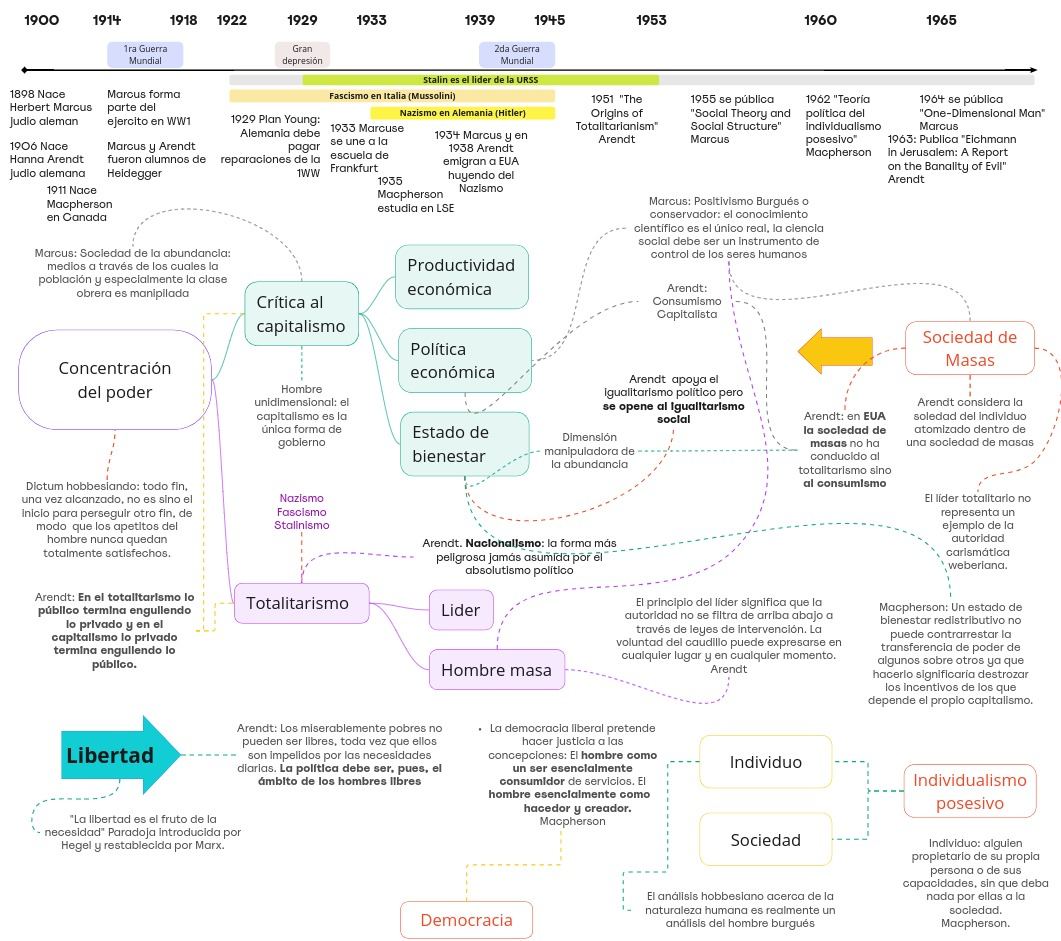
\includegraphics[keepaspectratio]{www/1_marcusarendtmac.jpg}}
\end{center}

\section{Liberalismo Combatiente}\label{liberalismo-combatiente}

\begin{quote}
Michael Oakeshott y Friedrich Hayek
\end{quote}

\begin{center}
\pandocbounded{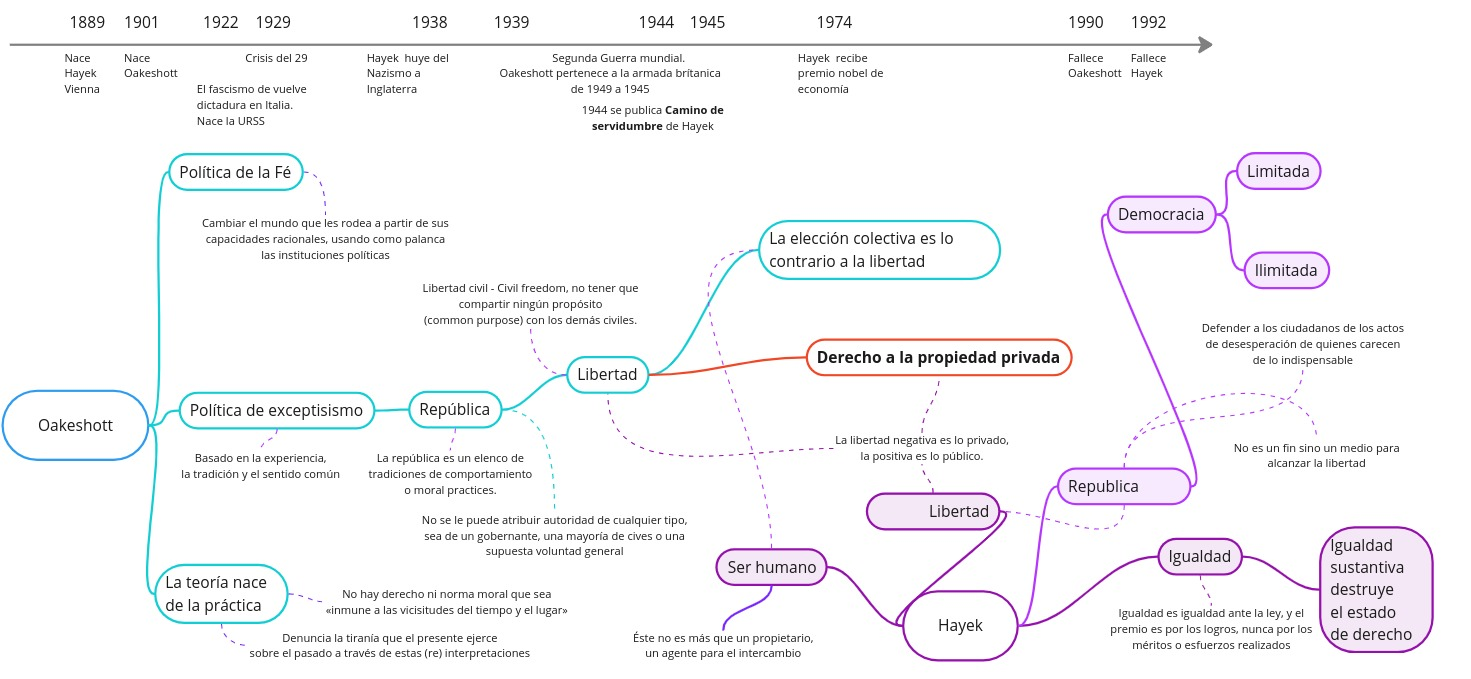
\includegraphics[keepaspectratio]{www/2_OakeshottHayek.jpg}}
\end{center}

\section{Racionalismo crítico y la sociedad
abierta}\label{racionalismo-cruxedtico-y-la-sociedad-abierta}

\begin{quote}
Karl Popper Figura~\ref{fig-popper} e Isaiah Berlin
Figura~\ref{fig-berlin}
\end{quote}

\begin{figure}

\caption{\label{fig-popper}}

\centering{

\pandocbounded{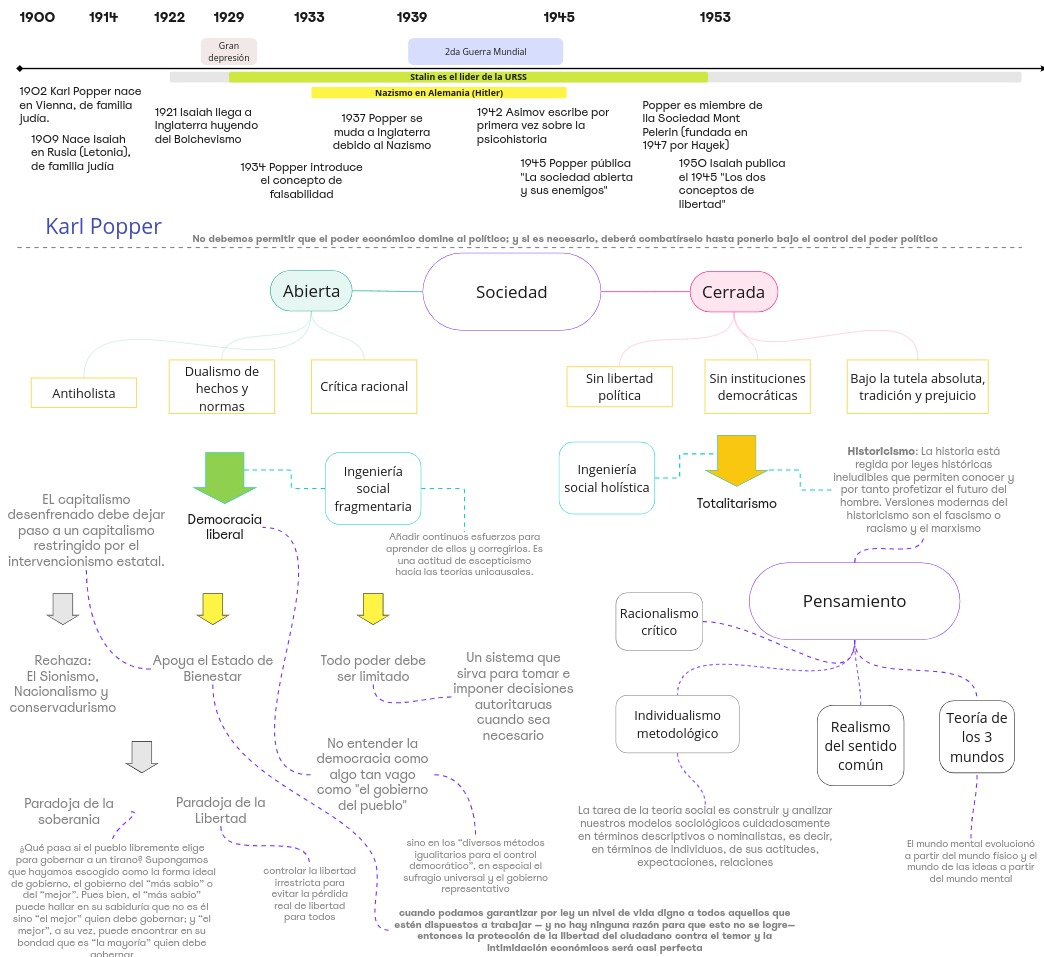
\includegraphics[keepaspectratio]{www/3_2_Popper.jpg}}

}

\end{figure}%

\begin{figure}

\caption{\label{fig-berlin}}

\centering{

\pandocbounded{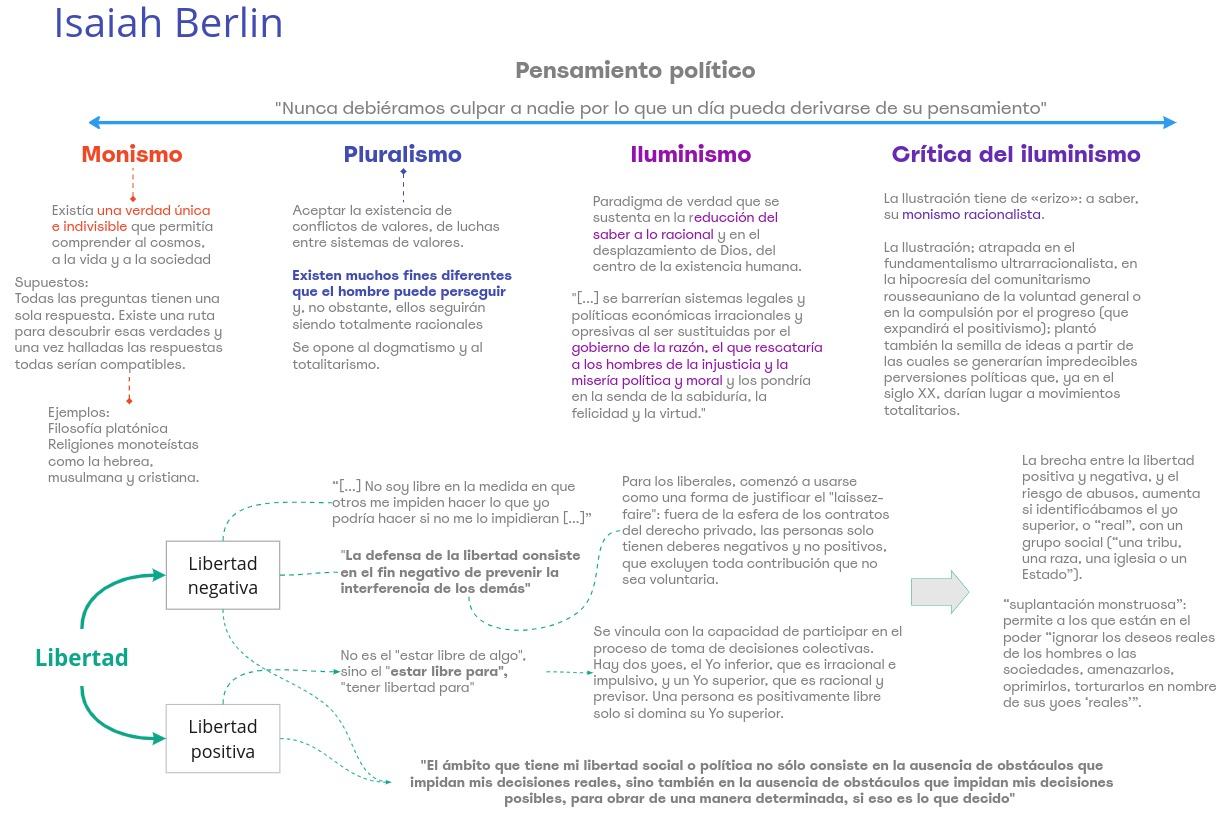
\includegraphics[keepaspectratio]{www/3_1_IsaiahBerlin.jpg}}

}

\end{figure}%

\chapter{Contemporáneos}\label{contemporuxe1neos}

Fuente principal: (\citeproc{ref-lessnoff2001}{Lessnoff 2001})

\section{John Rawls: Justicia
Liberal}\label{john-rawls-justicia-liberal}

\begin{itemize}
\item
  1958: artículo ``Justicia como equidad''

  Un razgo del contrato social sobre principios de justicia es que ``las
  partes contratantes sean lo suficientemente iguales en poderes y
  habilidades para garantizar que nadie es capaz de dominar a los
  demás'' Lo cual haría el contrato un contrato justo.

  La razón de todos los contratantes es disfrutar , en la mayor medida
  posible , los llamados bienes sociales primarios.
\item
  1971 publica el libro Una teoría de la justicia.

  \begin{itemize}
  \item
    Justicia social se logra si se consigue la distribución adecuada de
    los beneficios y cargas de la cooperación social.
  \item
    Estado: un contrato social sobre principios de justicia.
  \item
    Las desigualdades son supuéstamente inevitables en la estructura
    básica de cualquier sociedad {[}p5{]}.
  \item
    Sociedad: Una empresa cooperativa para la ventaja mutua. Cada
    persona prefiere una participación mayor a una menor.
  \item
    \textbf{Principios}

    \begin{enumerate}
    \def\labelenumi{\arabic{enumi}.}
    \item
      (\textbf{Primer principio}) Toda persona ha de tener igual derecho
      al sistema más extenso de libertades básicas iguales que sea
      compatible con un sistema semejante de libertades para todos.
    \item
      (\textbf{Segundo principio}) Las desigualdades sociales y
      económicas habrán de ser ordenadas tal que:

      \begin{itemize}
      \item
        Estén dirigidas hacía el mayor beneficio del menos aventajado
      \item
        Se vinculen a cargos y posiciones abiertos a todos bajo las
        condiciones de una equitativa igualdad de oportunidades.
      \end{itemize}
    \end{enumerate}

    \textbf{Libertades} básicas (\textbf{negativas}): Libertad política,
    libertad de discurso, libertad de reunión libertad de conciencia y
    de pensamiento, libertad personal junto con el derecho a la
    propiedad personal y libertad respecto a la detención y arresto
    arbitrario.

    \textbf{Democracia} constitucional
  \item
    Autorealización: uno de los bienes más importantes que un individuo
    puede disfrutar. La igualdad de oportunidades significa tener las
    mismas perspectivas de éxito independientemente de su posición
    inicial en la clase social. Hayeck mencionaba que esto no se podía
    lograr porque lo que se premia son los logros no los méritos.
  \item
    Prioridad de las necesidades materiales básicas:

    \begin{itemize}
    \item
      Deben estar cubiertas para todos
    \item
      Cualquier persona tiene igual derecho a un esquema plenamente
      similar de libertades para todos.
    \item
      Las oportunidades para lograr las posiciones sociales deseadas
      deben ser distribuidas por el sistema social de tal modo que logre
      maximizar las oportunidades de las clases más desfavorecidas.
    \item
      La \textbf{desigualdad económica} debe ser acordada de tal modo
      que logre maximizar la riqueza de la clase mas pobre.
    \item
      \textbf{Estado de bienestar}

      Es obligación del gobierno garantizar un mínimo social a cargo de
      mecanismos como la libre escolarización para todos, o bien a
      través de la enseñanza pública o subvencionando a las escuelas
      privadas.
    \item
      Ventajas de nacimiento: naturales (dotados), familia con riqueza,
      suerte.
    \end{itemize}
  \end{itemize}
\item
  1973 Libro Liberalismo político

  \begin{itemize}
  \item
    Modificación al \textbf{Primer principio}:

    Cualquier persona tiene el mismo derecho a un régimen completamente
    adecuado de libertades básicas, que sea compatible con un mismo
    esquema de libertades para todos.
  \item
    Sociedad: un sistema justo de cooperación a lo largo de un ciclo
    temporal completo.
  \item
    \textbf{Prioridad del derecho sobre el bien} (el acto correcto, lo
    bueno). El estado no debe apoyar una única concepción del bien
    (pluralidad).
  \item
    Ética de los mínimos
  \end{itemize}
\end{itemize}

\section{Robert Nozick: El estado
mínimo}\label{robert-nozick-el-estado-muxednimo}

\begin{itemize}
\item
  De 1938 a 2022. Nació en EUA de una familia descendiente de judíos
  (Wikipedia).
\item
  Catedrático de Harvard. Coincidió con Rawls en Harvard en 1963,
\item
  Presidente de la Asociación Filosófica Estadounidense
\item
  1960: Un compañero de la Universidad lo presentó a las ideas de Hayek
  con el libro ``The Consitution of Liberty''.

  \begin{quote}
  I also read some of the essays in ``Individualism and Economic
  Order'', especially the essays on rational calculation in a socialist
  society, and the impossibility of it. I thought, there must be
  something wrong with this and I'm going to find out what it is. The
  arguments bothered me. {[}\ldots{]} At first, though I had decided
  libertarianism was intellectually correct, I thought only bad people
  or mostly bad people would accept it, and that all the good people
  were on the left. So there was a period of time when I wouldn't tell
  people really quite what I believed. {[}Entrevista a Nozick de 1977{]}
  \end{quote}
\item
  1974: ``Anarquía, Estado y Utopía''

  Respuesta a ``A theory of justice'' 1971 de Rawls. Defiende un
  libertarismo extremo.

  Estado mínimo es aquel que se limita a proteger los derechos
  individuales y a garantizar la seguridad, sin intervenir en la
  economía más allá de lo necesario.Inspirado en el imperativo
  categórico de Kant ``Los individuos son fines y no solo medios''. El
  imperativo kantiano crea un caso ``prima facie'' contra la fuerza
  coercitiva, sin considerar quién sea el que la ejerce, o el propósito
  de tal fuerza. Para los anarquistas esto genera un supuesto
  concluyente contra el estado (intrínsecamente coercitivo).

  En un estado los individuos involucrados acturán de un modo interesado
  y racional.

  Privación del derecho natural de castigar a los que transgreden las
  normas (dada la tendencia de favoreserse a sí mismo cuando se es juez
  y parte).

  Teoría del título justo (Entitlement theory) :

  \begin{itemize}
  \item
    \emph{Just acquisition of holdings}

    Cualquiera que hace algo tras haber comprado o contratado los
    recursos que se necesitan en el proceso (\ldots) esta legitimado a
    poseerlo (Locke llama a estas transacciones la mezcla del trabajo de
    uno con los recursos apropiados). La apropiación no debe empeorar la
    situación de otros. Nozick: Las operaciones libres de un sistema de
    mercado no llegarían realmente a chocar con la condición de Locke.
    Incluso si el mercado libre, por ejemplo, no suministra nada a los
    incapacitados, no puede empeorar su situación. No pueden pretender
    más de lo que tienen, incluso si no tienen nada.
  \item
    \emph{Just transfer of holdings}:

    Una persona se convierte en el (nuevo) legítimo propietario de algo,
    que ya estaba legítimamente poseído, si y solo si, el propietario
    anterior se lo aliena libremente a él o ella - ya sea por donación,
    intercambio en el mercado, legado u otro procedimiento.

    ``Los impuestos sobre las ganancias del trabajo son equivalentes a
    los trabajos forzosos'' (transferencia obligada).
  \item
    \textbf{El derecho a la vida como derecho negativo:} Para Nozick, el
    derecho a la vida es un derecho negativo. Esto significa que otros
    tienen la obligación de abstenerse de quitarte la vida, pero no
    tienen la obligación de proporcionarte los medios para mantenerte
    con vida.
  \item
    Rectification of injustice:

    Una distribución de propiedades es justa sí y solo sí las
    propiedades fueron adquiridas por adquisición justa y transferencia
    justa.

    \begin{itemize}
    \tightlist
    \item
      Nozick (p231): ``Uno no puede servirse del análisis y de la teoría
      presentada {[}en este libro{]} para condenar ningún esquema
      particular de pagos por transferencia, a no ser que quede claro
      que no se puede aplicar ninguna consideración acerca de la
      rectificación de la injusticia para justificarlo''
    \end{itemize}
  \end{itemize}

  Utopía

  El mejor de los mundos posibles es el que permite que la mayor
  cantidad de gente posible viva lo más cerca posible de como desea
  vivir.

  \begin{itemize}
  \item
    Defensa de Nozick al ``Estado mínimo'':

    La visión libertaria puede crear un espacio para todos los estilos
    de vida, incluidos los anti-libertarios: las comunidades
    particulares podrían tener restricciones internas.

    ``No veo muy claro mi camino a través de estas cuestiones'' Nozick,
    The Examined Life pp 287-288.
  \end{itemize}
\item
  1981: Explicaciones filosóficas
\item
  1989: The Examined Life

  En el ensayo \emph{The sigzag of politics} expone:

  \begin{quote}
  ``La posición libertaria que una vez propuse me aparece ahora
  seriamente incorrecta''. La teoría de la justicia expuesta, en
  \emph{Anarquía, Estado y Utopía}, es en su mejor momento una defensa
  de solo uno de los valores de competencia (alusión a Isaiah Berlin),
  no un absoluto, pero uno que algunas veces puede ser invalidado o
  disminuido dentro de los intercambios.
  \end{quote}
\item
  2001: Invarianzas
\item
  1950: Hayek se unió a la universidad de Chicago
\end{itemize}

\section{Jürgen Habermas: Ética del discurso y
democracia}\label{juxfcrgen-habermas-uxe9tica-del-discurso-y-democracia}

Nació en 1929 en Düsseldorf, Alemania. En 1933 su padre se volvió
miembro del partido Nazi NSDAP
{[}\href{https://en.wikipedia.org/wiki/J\%C3\%BCrgen_Habermas}{Wikipedia,
2024}{]}. Habermas fue un \emph{Jungvolkführer} de la Juventud de
Hitler. Director del Instituo Max Planck en 1971. Elegido como
\emph{Foreign Honorary Member} de la \hyperref[0]{\emph{American Academy
of Arts and Sciences}} en 1984.

\begin{quote}
Habermas argues that his speech disability made him think differently
about the importance of deep dependence and of communication {[}(2008).
``First''. Between Naturalism and Religion: Philosophical Essays,
Wikipedia{]}
\end{quote}

\begin{itemize}
\item
  1968 Habermas publica ``Conocimiento e interés''

  Obra escrita contra el ``positivismo'' y la ``ciencia social
  positivista''.

  El \emph{positivismo} presupone:

  \begin{itemize}
  \item
    La ciencia no aporta más que conocimiento del mundo tal como
    actualmente es, así como que el acercamiento científico es el mejor
    y único modo de acceder al conocimiento y, en esa medida ha de ser
    aplicado al ámbito social del mismo modo que ya lo ha sido con exito
    en la naturaleza, con objeto de producir ciencia social.
  \item
    La ciencia incluyendo a la ciencia social es necesariamente una
    ciencia libre de valores (como Max Weber afirmaba).
  \end{itemize}
\item
  Refutación de Hebermas:

  \begin{itemize}
  \item
    La ingenuidad estriba en que niega la relación existente entre
    conocimiento e interés, es decir, la dependencia del conocimiento
    humano de intereses y, por tanto, de fines y valores.
  \item
    Si la ciencia natural se estructura de este modo es porque, más
    bien, esta organización es inherente a nosotros mismos y al carácter
    técnico de nuestro interés por la naturaleza. ``\textbf{Las ciencias
    empíricas contienen información acerca de la realidad desde el punto
    de vista del posible control técnico}'' {[}Pierce y Dilthey{]}.
  \item
    Es a través del trabajo y de sus exigencias donde el hombre llega a
    conocer su medio ambiente natural, acercándose a Marx. Pero rechaza
    la extensión de este ámbito al social, siguiendo la Escuela de
    Franskfurt.
  \item
    Entendimiento mutuo orientado a la acción (Prácticamente efectivo):
    conocimiento e interés propio del ámbito social en lugar de ciencias
    sociales

    \begin{itemize}
    \item
      Conocimiento constitutivo: Todos los seres humanos lo adquieren a
      través de los progresos en socialización, los cuales proporcionan
      una imagen estructurada lingüísticamente de su mundo social y les
      capacita para participar en él.
    \item
      Conocimiento científico: Esfuerzo por aprender o comprender el
      mundo mental compartido que estructura las interacciones de los
      seres humanos sociales. Las ciencias hermenéuticas no están en
      situación de contestar a un tercero de los intereses humanos:

      \begin{itemize}
      \item
        Hermenéuticas
      \item
        Histórico-hermenéuticas y
      \item
        Ciencias culturales
      \end{itemize}
    \end{itemize}
  \item
    Tiene dos vertientes, la filosófica y la política:

    \begin{itemize}
    \item
      La doctrina positivista de la ciencia libre de valores (que
      implica que los juicios de valor no son conocimiento, toda vez que
      estos no son ni siquiera objeto de estudio racional) reduce las
      elecciones políticas a decisiones arbitrarias en manos de líderes,
      en lugar de promover una discusión democrática racional y un
      posible acuerdo (sobre la acción ilustrada), hasta en el marco de
      sistemas políticos opuestamente democráticos. {[}Toward a Rational
      Sociaety, 1971, pp67-68{]}
    \item
      Implica que la política racional debe adoptar la forma
      instrumental de aplicación de leyes estructuradas bajo un control
      técnico, presumíblemente, bajo seres humanos. La ciencia social
      técnica entendida en términos positivistas se convierte, a ojos de
      Habermas, en un instrumento para que algunas personas ejerzan un
      cierto poder sobre otras (casta tecnocrática). \emph{Los
      tecnócratas usan la ciencia y la tecnología como una ideología}.

      \emph{El conocimiento técnico es un conocimiento que permite que
      el objeto cognoscitivo sea tratado como un medio para los fines de
      aquel que usa el conocimiento}.
    \end{itemize}
  \item
    Ciencias naturales nomológicas: ciencias sistemáticas de la acción
    social (economía, ciencias políticas, sociología entre otras):

    \begin{itemize}
    \item
      Identifica a muchas leyes sociales como armas para el ejercicio
      del poder (de los poderosos sobre los más indefensos) en
      estructuras sociales dadas; falsa pretensión de leyes universales
      e inalterables como instrumentos para perpetuar la desigualdad.

      Una ley sociológica del tipo \emph{``si X se realiza, la gente
      hará Y'':} puede ser usada para controlar o manipular a la gente
      y, en esa medida, expresa relaciones de dependencia. Si la gente
      creyera que ninguna estructura social alternativa podría modificar
      esa situación, o que no existiera una manera de resistir a ese
      resultado Y - Si se cree en esto, la ley universal podría
      convertirse en una suerte de profecía \emph{self-fulfilling},
      susceptible de hacerse real en virtud de sus propios presupuestos
      y por tanto, a congelar las relaciones de dependencia que en un
      principio pueden ser objeto de transformación (Leído en
      (\citeproc{ref-lessnoff2001}{Lessnoff 2001}) página 293, fuente
      inicial Hebermas (\citeproc{ref-vallance1973}{Vallance, Habermas,
      y Shapiro 1973}) p310).
    \end{itemize}
  \item
    Remedio ``La conciencia Reflexiva'': este tipo de auto-reflexión
    crítica es emancipadora: sirve al interés cognitivo emancipador
    porque produce un conocimiento susceptible de liberar a los hombres
    de la dependencia de los poderes hipostasiados.
  \end{itemize}
\item
  Libro ``Crisis de legitimación del capitalismo tardío''
\item
  1981: The theory of Communicative action.

  \begin{itemize}
  \tightlist
  \item
    El estado de bienestar es un caso modélico de la colonización del
    mundo de la vida por parte del sistema. Implica la claudicación de
    la autonomía en beneficio del bienestar.
  \end{itemize}

  Acción teleológica en términos de Max Weber ``racionalidad de fines''
  o ``racionalidad instrumental''.

  \begin{itemize}
  \item
    Acción estratégica
  \item
    Acción comunicativa: Interacción entre, al menos, dos sujetos
    capaces de discurso {[}\ldots{]} que establecen relaciones
    interpersonales {[}\ldots{]} los actores buscan alcanzar un
    entendimiento acerca de la situación de la acción y de sus planes
    con objeto de coordinar estas acciones por medio de un acuerdo {[}pp
    10,14{]}. Según (\citeproc{ref-lessnoff2001}{Lessnoff 2001}) se
    presupone que \textbf{la acción comunicativa se corresponda con su
    apropiada forma de racionalidad: la racionalidad comunicativa}; y
    que Habermas lo usa para plantear una crítica de la concepción
    sociohistórica weberiana de la racionalización característica de la
    civilización occidental.
  \item
    La racionalidad comunicativa, a juicio de Habermas, es más
    fundamental y amplia que la instrumental analizada por Weber
    {[}p.10{]}. La racionalidad instrumental -adaptación eficiente de
    medios a un fin no es un logro peculiarmente humano, lo que es
    peculiar es el lenguaje. La racionalidad instrumental se incrementa
    naturalmente, gracias a la capacidad humana de hablar, discutir y
    convencer racionalmente.

    \textbf{Validez susceptible de crítica} de tal suerte que cualquier
    acción orientada a fines descansa en creencias acerca del mundo que,
    si son verdaderas, convierten la acción en racional. \textbf{La
    racionalidad esta en este sentido ligada al acuerdo o al consenso}.
    Habermas con la idea de ``corrección'' cree que la racionalidad
    implica una orientación o una intención hacia el consenso
    discursivo. El uso instrumental o estratégico del lenguaje va más
    allá de la función original del lenguaje.
  \end{itemize}
\item
  1962: Libro ``The structural transformation of the public sphere''

  \begin{itemize}
  \item
    Esfera privada: vida familiar, vecindad y la asociación voluntaria.

    \begin{quote}
    La esfera pública fue subsumida en el marco del consumo, una empresa
    conducida por el mercado que en parte consiente y en parte manipula
    a una masa cultural tan acrítica como apolítica. {[}p160{]}
    \end{quote}
  \item
    La democracia parlamentario moderna consiste en gran medida en la
    manipulación de los votantes en manos de las élites políticas.
  \item
    En un estado de bienestar social que fundamentalmente administra,
    distribuye y mantiene. Los intereses ``políticos'' de los ciudadanos
    están constantemente subsumidos en actos administrativos {[}p
    211{]}.
  \end{itemize}
\item
  1992: Libro Factibilidad y validez
\end{itemize}

\chapter{Concepciones de lo
político}\label{concepciones-de-lo-poluxedtico}

La fuente principal, de esta sección, es
(\citeproc{ref-garcia2011}{Garcia, Kohn, y Astorga 2011}).

\section{Antonio Francesco Gramsci}\label{antonio-francesco-gramsci}

Born in 1981 -- 1937. Gramsci died on 27 April 1937, at the age of 46.
Italian marxist philosopher, linguist, journalist. He was part of the
italian Communist Party and a vocal critic of Mussolini. He was in
prision from 1926 -- 1937. The failure of the workers' councils to
develop into a national movement convinced Gramsci that a Communist
party in the Leninist sense was needed.

\begin{quote}
George Orwell's novel ``1984'' was published in 1949 (Foucault was 23
years old at that time).
\end{quote}

\subsection{Antonio Gramsci en los estudios culturales de Raymond
Williams}\label{antonio-gramsci-en-los-estudios-culturales-de-raymond-williams}

\begin{quote}
Fuente: (\citeproc{ref-antonio}{{«Antonio Gramsci en los estudios
culturales de Raymond Williams»}, previsto})
\end{quote}

``\textbf{For twenty years we must stop this brain from functioning''}
(\citeproc{ref-gramsci2012}{Gramsci y Gramsci 2012})

Do Critical Theory and Gramsci have anything in common with Foucault?
Gramsci and first generation Critical Theorists were both sympathetic to
the workers' council movement of the 1920s and also accept that our
ability to understand the world is rooted in the fact that we also
produce that world. This idea goes back to the tradition of Vico and was
elaborated in Marx' and Engels' German Ideology. It emphasizes, in
contrast to Habermas's misinterpretation of Marx, that such production
goes beyond labour to include speaking, governing, having sex, begetting
children, struggling and revolting.

Foucault rejected the idea of critical theory as a theory of a social
totality

People could be seen as exploited and subordinated not only by the
control of their work but also by and through their cultural practices.
In the perspective of Walter Benjamin, Bertolt Brecht or Theodor Adorno,
culture was the barbarian triumph of the ruling classes -- domination
includes also the power and the right to define what culture and
legitimized knowledge is.

\subsubsection{``Ideal Average'' on the economic
context:}\label{ideal-average-on-the-economic-context}

Capitalism: The logic of capital in a capitalist system often
prioritizes profit maximization and efficiency. This can lead to
inequalities, exploitation, and environmental degradation.

Socialism: In a socialist system, the logic of capital might be modified
to prioritize social welfare and equality. However, the concept of
capital itself may still exist, albeit in a different form.

Mixed Economy: Many economies combine elements of capitalism and
socialism. The ``ideal average'' would depend on the specific balance
between these elements.

\subsubsection{Similiaritys between Gramsci's theory of hegemony and
Orwell's dystopian novel,
1984.}\label{similiaritys-between-gramscis-theory-of-hegemony-and-orwells-dystopian-novel-1984.}

Cultural hegemony: Both Gramsci and Orwell highlight the importance of
cultural control in maintaining power.

Manipulation of language: In both cases, language is used to shape
perception and control thought.

Propaganda: Both emphasize the role of propaganda in maintaining the
dominant ideology.

Surveillance: Orwell's novel demonstrates how surveillance can be used
to enforce conformity and prevent dissent.

\begin{quote}
``For many he also seems to explain why workers under advanced
capitalism have not behaved the way Marx said they would and to offer a
more succesful revolutionary strategy'' (\citeproc{ref-lears1985}{Lears
1985})
\end{quote}

\subsection{Cultural hegemony today, from cultural studies to critical
pedagogy}\label{cultural-hegemony-today-from-cultural-studies-to-critical-pedagogy}

\begin{quote}
Fuente: (\citeproc{ref-cortuxe9s-ramuxedrez2015}{Cortés-Ramírez 2015})
\end{quote}

Hegemony is not equal to (\ldots.) ideology, consciousness formations of
the ruling class are not reduced, but include the relations of
domination and subordination, according to (\ldots..) practical
consciousness configurations, as an effective saturation of the process
of life in full (\ldots) hegemony is a body of practices and
expectations regarding the whole of life. Our senses and energy
(\ldots..) define perceptions we have of ourselves and our world. It is
a vivid system of meanings and values. To the extent they are
experienced as practices (they) appear to confirm each other. It is a
sense of reality for most people in society (\ldots) (Williams 1977:
109).

As Edward Said has argued in his book Orientalism, the suffering of the
people is the direct effect of cultural exchange between partners who
are aware of the inequality of this exchange (Said, 1978, p.~95).

Said, E (1993). Culture and Imperialism, London: Chatto \& Windus.

The term hegemony derives from the Greek verb eghesthai, meaning ``to
drive'', ``to be the guide'', ``to be the boss''; or maybe from the verb
eghemoneno, that means ``to guide'', ``to precede'', ``to drive'', and
hence ``to stay ahead'', ``to command'', ``to rule''. At the time of the
Peloponnesian War, reference was constantly made to the ``hegemonic''
city, the town that managed the alliance of Greek cities fighting each
other.

For Lenin, the bourgeoisie has always attempted to separate Politics
from Economics, because this class understands very well that if it
manages to keep the working class within the corporate framework, no
serious danger may threaten its hegemony (VVAA, 1969: 20).

Tthe basis of the concept of hegemony was established by the principles
defined by Lenin during the Third International. Gramsci emphasized the
need of concessions and sacrifices of the proletariat to its allies to
be able to exert hegemonic direction over them.

Coercion needs to be accompanied by consent.

Commitment offers important concrete possibilities. Force can be used
against enemies, but not against those allied groups that need to be
quickly assimilated, and whose good faith, trust and enthusiasm are
needed (Gramsci, 1975, p.~62).

It may be that war is the continuation of politics by other means. But
it may also be that politics is becoming the continuation of war by
other means (Foucault, 1997, pp.~16 and 41; Pandolfi, 2002,
pp.~391-410).

\section{Michel Foucault}\label{michel-foucault}

He was a French historian of ideas and philosofer. Lecturer on Tunis
from 1966 to 1968. He died from complications of HIV/AIDS in Paris.
First cases of HIV were discovered in France at 1983 by Pasteur
institute. He described himself as a ``juvenile delinquent''.

\begin{quote}
I wasn't always smart, I was actually very stupid in school \ldots{}
There was a boy who was very attractive who was even stupider than I
was. And to ingratiate myself with this boy who was very beautiful, I
began to do his homework for him---and that's how I became smart, I had
to do all this work to just keep ahead of him a little bit, to help him.
In a sense, all the rest of my life I've been trying to do intellectual
things that would attract beautiful boys {[}Foucault, 1983{]}
\end{quote}

\subsection{Poder, disciplina e
ilegalismos}\label{poder-disciplina-e-ilegalismos}

\begin{enumerate}
\def\labelenumi{\arabic{enumi}.}
\item
  Power is not something you possess, power is something you wield.

  No es una propiedad sino una estrategia; no es el privilegio adquirido
  o conservado de la clase dominante, sino el efecto de conjunto de sus
  posiciones estratégicas.
\item
  El poder no esta localizado en el Estado; por el contrario, el Estado
  aparece como un efecto de conjunto o una resultante de una
  multiplicidad de engranajes y de núcleos que se sitúan a un nivel
  completamente distinto y que constituyen de por sí una microfísica del
  poder.
\item
  Es falso que el poder encarnado en el Estado esté subordinado a un
  Modo de Producción como infraestructura.
\item
  El poder carece de esencia, es operatorio. No es atributo sino
  relación.

  El poder enviste a los dominados, pasa por ellos y mediante ellos, se
  apoya en ellos, del mismo modo que ellos, en su lucha contra él, se
  apoyan a su vez en las influencias que ejerce sobre ellos.
\item
  El poder más que reprimir, produce realidad y, más que ideologisar,
  abstraer u ocultar, produce verdad.
\item
  El poder de Estado no se expresa en la Ley.

  La ley siempre es una composición de ilegalismos que ella diferencia
  al formalizarlos.
\end{enumerate}

\begin{quote}
El cuerpo como objeto y blanco del poder
\end{quote}

``Docilidad, combinación ingeniosa entre el cuerpo analizable y el
cuerpo manipulable''. Sometimiento, utilidad, transformación y
perfeccionamiento se fusionan para producir los cuerpos dóciles.

\begin{quote}
``La delincuencia funciona como un observatorio político'' Foucault
\end{quote}

Teorías de los ilegalismos:

\begin{itemize}
\item
  La democracia del objeto
\item
  La estructura conceptual
\item
  La explicación del cambio social
\end{itemize}

El poder disciplinario, propio de la sociedad carcelaria y normativa y
de las instituciones de encierro en general, representa un nuevo periodo
de la historia punitiva donde se han colonizado los ilegalismos
populares y \textbf{ha surgido un ilegalismo controlado llamado
delincuencia}.

\emph{La apreciación jurídica de la propiedad originó un desplazamiento
de los ilegalismos, del ataque a los cuerpos al ataque a los bienes}. La
crisis de los ilegalismos populares exigió a los reformadores una nueva
estrategia para redistribuir y administrar los ilegalismos.

\begin{quote}
Suavizamiento de los crímenes antes del suavizamiento de las leyes.
\end{quote}

Cuando los reformadores plantearon la abolición de la pena capital,
\textbf{lo hacían, no porque querían castigar menos, sino porque querían
castigar mejor}.

\begin{quote}
\emph{los diferentes estratos sociales tenían cada cual su margen de
ilegalismo tolerado. Este estaba tan profundamente anclado que tenías su
coherencia y su economía propia.}
\end{quote}

Una parte de la burguesía había aceptado sin demasiados problemas el
ilegalismo de los derechos, lo soportaba mal cuando se trataba de lo que
consideraba sus derechos de propiedad.

Ilegalismos populares:

\begin{itemize}
\item
  Político
\item
  Resistencia al movimiento de industrialización

  Las prácticas ilegalistas se oponen a la ley misma y a la justicia
  encargada de aplicarla, a los empresarios que multiplican las maquinas
  y bajan salarios; se oponen al régimen de la propiedad territorial
\item
  Efectos de las crisis económicas

  \begin{quote}
  \textbf{El lumpen} es un término que se originó en el marxismo para
  referirse a un sector de la sociedad que se encuentra en una posición
  socialmente marginal y desfavorecida.
  \end{quote}
\end{itemize}

Sería ingenuo creer que la ley se ha hecho para todo el mundo en nombre
de todo el mundo; es más prudente reconocer que se ha hecho para algunos
y que recae sobre otros; que en principio obliga a todos los ciudadanos,
pero que se dirige principalmente a las clases más numerosas y menos
ilustradas, que a diferencia de lo que ocurre con las leyes políticas o
civiles, su aplicación no concierne por igual a todo el mundo.

\begin{quote}
Relations of power `are the immediate effects of the divisions,
inequalities, and disequilibriums which occur in the latter {[}social
relations per se{]}, and conversely they are the internal conditions of
these differentiations' which may be determined by law, status, economic
appropriation, processes of production, language, culture, knowledge or
competence (\citeproc{ref-deacon1998}{Deacon 1998}).

Every human relation is to some degree a power relation, it power is
produced \ldots{} in every relation from one point to another; it is
everywhere; not because it embraces everything, but because it comes
from everywhere (Foucault 1981a:93).
\end{quote}

\begin{quote}
``When power blends into desire and desire blends into power, let's
forget them both'' (\citeproc{ref-baudrillard2007}{Baudrillard y
Lotringer 2007}).
\end{quote}

\chapter{Comunitarismo}\label{comunitarismo}

\section{Los Verbos de la democracia}\label{los-verbos-de-la-democracia}

\begin{quote}
Notas de sobre la ponenecia Michelangelo Bovero, traducidas al español
por José Fernández Santillán, (\citeproc{ref-bovero1998}{Bovero 1998}).
\href{https://www.eld.edu.mx/michelangelo-bovero-3/}{Bovero} fue alumno
de Norberto Bobbio.
\end{quote}

\begin{itemize}
\item
  \textbf{Gramática}: conjunto de los elementos fundamentales y de las
  nociones primarias de cualquier materia, o en el sentido más cercano
  al específico y literal.
\item
  \textbf{Torre de Babel}: la humanidad intentó construir una torre que
  llegara al cielo y fue castigada con la confusión de lenguas, sirve
  como analogía para describir la situación actual de la política en
  muchos lugares del mundo.
\end{itemize}

\subsection{Juego democrático}\label{juego-democruxe1tico}

Conjunto de las actividades interdependientes en las que se desarrolla
la ``vida pública'' de una colectividad, las reglas democráticas son las
reglas del juego.

\begin{quote}
La democrática está programada para producir decisiones ``con el máximo
de consenso y con el mínimo de imposición'' Bobbio
\end{quote}

Según teoría de juegos \emph{sería un ``juego mixto'', en el que
competencia y cooperación se intersectan.}

El verbo de la democracia es sustancialmente sólo uno, escalar, y su
objeto es alcanzar la posición desde la que se ``domina'' todo.

Hasta abajo de la pirámide están los ciudadanos, \emph{el juego
democrático inicia con el acto de \texttt{elegir}}. Enseguida el juego
pasa a los elegidos, personas seleccionadas por los ciudadanos electores
y designadas por esos ciudadanos para formar los órganos institucionales
de la colectividad, al parlamento. Al papel de quienes han sido electos,
en cuanto tales, es el de \texttt{representar} a los ciudadanos, ante
todo en el sentido elemental de \emph{``sustituirlos''} en las fases
ulteriores del juego democrático. La función específica del parlamento
consiste en \texttt{deliberar} acerca de las cuestiones públicas.
\texttt{Decidir}, es la actividad final, no tendría sentido elegir,
representar, deliberar, si no se llegase a decidir.

La vida pública de una colectividad puede ser considerada como
democracia si, las decisiones políticas \emph{no llueven de arriba sobre
los ciudadanos}, sino que brotan de \emph{un ``juego'' que ellos mismos
han iniciado y controlado.}

\begin{quote}
La costumbre produce ceguera: la utilización cotidianamente repetida
ofusca ante nuestros ojos el sentido de las palabras, disminuye el
control sobre la comunicación y favorece la difusión de los equívocos.
Hegel
\end{quote}

Los cuatro verbos de la democracia:

\begin{itemize}
\item
  \textbf{Elegir} \emph{(elegire)}: es el acto de designar y elevar.

  El instituto político electoral era considerado como típico de la
  aristocracia; aristos en griego significa ``el mejor'', y aristokratía
  ``el poder de los mejores'':

  \begin{quote}
  ¿Debemos concluir que en las democracias representativas, donde el
  juego es abierto, en realidad son (cuando todo va bien) aristocracias,
  o (cuando la selección se hace mal) oligarquías electivas?
  \end{quote}

  El juego democrático debe ser concebido, según teoría de juegos, como
  un ``juego repetido'': la repetición de las elecciones conforme a
  intervalos regulares --repetición que implica la posibilidad de la
  reelección o revocación de los elegidos- es lo que hace compatible (en
  principio) con la democracia el acto de por sí aristocrático, u
  oligárquico, de elegir.

  El acto de elegir, debe desarrollarse de acuerdo con las reglas de un
  juego justo, \emph{fair play}. Ningún ciudadano debe ser excluido de
  él.
\item
  \textbf{Representar} (\emph{repraesentare}): hacer sensible o
  inteligible algo abstracto mediante algo concreto, p.e. un presidente,
  ``representa'' un Estado.

  Representativo pero no democrático era el Estado liberal clásico, que
  tenía un parlamento pero éste no estaba formado con base en el
  sufragio universal equitativo. En un juego dmocrático, el significado
  de ``actuar a nombre y por cuenta de'' se se debe conjugar con uno de
  los significados originarios: reflectar, reflejar o reproducir
  fielmente.

  \begin{quote}
  Los elegidos al parlamento ``representan'' a los ciudadanos,
  electores, en la medida en que el parlamento en su conjunto,
  reproduzca las diversas tendencias y orientaciones políticas presentes
  en el país.
  \end{quote}
\item
  \textbf{Deliberar} (\emph{deliberare}): ha adquirido el sentido
  predominante y metafórico de ``ponderar''.

  La discusión de las diversas tesis o puntos de vista, la ponderación
  de los argumentos en pro o en contra, y el intento de persuasión
  recíproca entre los respectivos proponentes.
\item
  \textbf{Decidir} (\emph{decidire}): significa literalmente cortar,
  truncar, concluir abreviando; lo que es ``abreviado'', que
  ``concluye''.

  \begin{quote}
  Cualquier colectividad política debe poder llegar, para todo problema
  de relevancia pública, a una única voluntad, válida y obligatoria para
  todos, superando el conflicto.
  \end{quote}
\end{itemize}

La decisión es democrática, es fruto de un juego democrático, cuando en
el momento de la deliberación, participaron con iguales oportunidades de
valoración y persuasión recíproca los representantes de todas las
opiniones políticas; y esto presupone, a su vez, que la
representatividad de los órganos colegiados deliberantes esté
garantizada por mecanismos electorales no distorsionantes y no
penalizantes para nadie.

\begin{quote}
El principio de mayoría es un buen método para decidir, pero también
puede ser un pésimo método para elegir.
\end{quote}

\subsection{Poder ejecutivo}\label{poder-ejecutivo}

\begin{quote}
El lenguaje mismo denuncia que hay una incongruencia: \emph{de ninguna
manera gobernar significa ejecutar}. Un poder puramente ejecutivo, por
definición, no decide nada políticamente relevante; a lo más toma
decisiones técnicas sobre los medios, pero no determinaciones políticas
acerca de los fines colectivos.
\end{quote}

De acuerdo a Bovero, \emph{``decidir, es una actividad, en la mayoría de
los casos compartida --en modos diversos y complicados-- por dos sujetos
institucionales, el parlamento y el gobierno}.

\begin{itemize}
\item
  \textbf{Gobernar} (\emph{Kybernetes}): Calcado por el latín como
  \emph{gubernator}, kybernetes y gubernator significan literalmente el
  piloto de la nave; quien ejerce el arte de gobernar es literal y
  originariamente ``quien lleva el timón''.

  Quien ejerce la actividad de regir es quien traza la línea. El verbo
  griego correspondiente, \emph{árcho}, en el sentido originario
  indicaba ``yo soy el primero de la fila y por consiguiente guío,
  conduzco la marcha, dirijo''. Es quién establece los fines y los
  objetivos colectivos, y en este sentido ``manda'', ``detenta la
  decisión última''.
\end{itemize}

Las tres metáforas canónicas de la acción de los gobernantes:

\begin{itemize}
\item
  Timonel (el jefe): quien traza la ruta, o sea, establece los fines
  colectivos.
\item
  Pastor: quien guía la marcha, quien formula la orientación común.
\item
  Tejedor: quien entrelaza los hilos de la convivencia, o sea, produce
  cooperación social.
\end{itemize}

\begin{quote}
Un problema político de los ``gobernantes'' en sentido amplio es
producir decisiones colectivas coherentes.
\end{quote}

Actualmente, se tiene un dilema, entre aceptar un gobierno más
democrático, pero equívoco, con consecuentes daños sociales, o bien se
busca un gobierno unívoco, pero menos democrático, con consecuentes
peligros de autoritarismo en las decisiones.

Frente a los partidarios de los gobiernos fuertes, la democracia del año
2000 consiste en el hecho de que el presidente o el jefe del gobierno es
elegido directamente por los ciudadanos bajo la regla de la mayoría,
aquí Bovero concluyé que, esa ya no es una democracia, porque allí se
trastoca el sentido correcto de los verbos de la democracia, los
regímenes con gobierno fuerte corren el riesgo de ser autocracias
electivas, donde el parlamento ya no delibera, sino que se convierte
simplemente en un contrapoder que controla la actuación del gobierno.

\subsection{Teoría de juegos}\label{teoruxeda-de-juegos}

\begin{quote}
\textbf{Theory of rational choice}: the action chosen by a
decision-maker is at least as good, according to her preferences, as
every other available action (\citeproc{ref-osborne2004}{Osborne 2004}).
\end{quote}

\begin{quote}
\textbf{Definition.} Game theory is a study of mathematical models of
conflict and cooperation between rational decision makers. Rationality
means that each individual's decision-making behavior would be
consistent with the maximization of subjective expected utility, if the
other individuals' decisions were specified.
(\citeproc{ref-myerson1984}{Myerson 1984})
\end{quote}

Rationality implies that individuals know the strategies available to
each individual, have complete and consistent preferences over possible
outcomes, and they are aware of those preferences, \emph{we refer to the
decision-makers as players}.

\begin{itemize}
\item
  Juegos cooperativos: Los jugadores actúan como grupo y coordinan sus
  acciones para su beneficio mutuo.
\item
  Juegos no cooperativos: Los jugadores son rivales y cada uno actúa en
  su propio interés, sin pensar en la suerte de los otros jugadores.
\end{itemize}

En los \textbf{\emph{juegos mixtos}} sólo la cooperación permite
asegurar la obtención de beneficios, pero el conflicto de intereses
determinado por la estructura de recompensas introduce un factor de
competitividad que interfiere en el proceso de coordinación, hasta el
punto de que si tal conflicto no se dirime de alguna forma mediante
algún procedimiento de ajuste, la cooperación y, en definitiva, el
resultado positivo, pueden verse claramente en peligro.

\section{Republicanismo, liberalismo y
comunitarismo}\label{republicanismo-liberalismo-y-comunitarismo}

\begin{quote}
Fuente: (\citeproc{ref-uscangabarradas2016}{Uscanga Barradas 2016})
\end{quote}

El comunitarismo tuvo su auge en la decada de 1980 y se inspiró en gran
medida en Aristóteles y Hegel, nació, al igual que el neorepublicanismo,
como alternativa al modelo político liberal. El comunitarismo tiene como
una de sus características el holismo ontológico, la realidad debe ser
entendida como un todo interconectado, y la afirmación de una naturaleza
humana social.

Los comunitaristas apoyan políticas del bien común, conciben al
individuo como un ser incompleto perfectible solo en la sociedad a
partir de la participación que funciona como puente que le permite a la
parte integrarse al todo.

\begin{itemize}
\item
  Individuo

  \begin{itemize}
  \item
    (liberalismo) Rawls indica que \emph{el yo antecede a sus fines},
    los individuos tienen la capacidad de cuestionar su pertenencia en
    cualquier grupo, entidad o comunidad, hasta el punto de separarse de
    ella, si así lo prefieren.
  \item
    (comunitarismo) Charles Taylor: nuestra entidad se encuentra
    profundamente marcada por nuestra pertenencia a ciertos grupos. El
    hombre es un animal social, un \emph{zoon politikon} que requiere
    para su existencia de la \emph{polis,} para afirmar su autonomía
    moral.
  \end{itemize}
\end{itemize}

\begin{quote}
No hay un solo sujeto que pueda ser totalmente libre, sino solamente
libre de elegir un entorno diferente: \emph{``¿Podríamos imaginarnos
individuos que no tuvieran vinculaciones de ningún tipo? ¿Individuos que
no estuvieran determinados por la clase, la religión o el género, sino
que carecieran de identidad y fueran completamente libres?''}. (Walzer,
2004, p.~35).
\end{quote}

\begin{itemize}
\item
  Libertad

  \begin{itemize}
  \item
    (republicanismo) Libertad como no dominación, ausencia de
    dominación.
  \item
    (liberalismo) Libertad como no interferencia: ausencia de
    interferencia.
  \item
    (comunitarismo) libertad basada en la pluralidad, es decir, la
    alteridad y colectividad.
  \end{itemize}
\item
  Sociedad multicultural

  (comunitarismo) La sociedad multicultural ha dividido nuevamente a las
  sociedades, tal y como sucede con el individualismo, en cada uno con
  una identidad personal separada del resto: indígenas con indígenas,
  feministas con feministas, etc; es contraproducente que estas
  sociedades divididas en diversas identidades trabajen de forma aislada
  al resto de una comunidad en lugar de trabajar todos ellos en común,
  sin necesidad de perder esa identidad
  (\citeproc{ref-universidaddeguadalajaramuxe9xico2021b}{García Solano
  2021}).

  \begin{quote}
  ``{[}\ldots{]} el que yo descubra mi propia identidad no significa que
  la haya elaborado en el aislamiento, sino que la he negociado por
  medio del diálogo {[}\ldots{]}, con los demás''. (Taylor, 2009,
  p.~65).
  \end{quote}
\end{itemize}

\chapter{Pragmatismo}\label{pragmatismo}

\begin{quote}
``Lo que distingue al hombre civilizado del bárbaro es advertir la
validez relativa de las propias convicciones y defenderlas, sin embargo,
resueltamente. Pedir más que eso es, quizás, una necesidad metafísica
profunda e incurable; pero permitir que ello determine nuestra práctica
es síntoma de una inmadurez moral y política igualmente profunda, y más
peligrosa'' (\citeproc{ref-rorty2020}{Rorty 2020})
\end{quote}

\subsubsection{Contexto histórico}\label{contexto-histuxf3rico}

\begin{center}
\pandocbounded{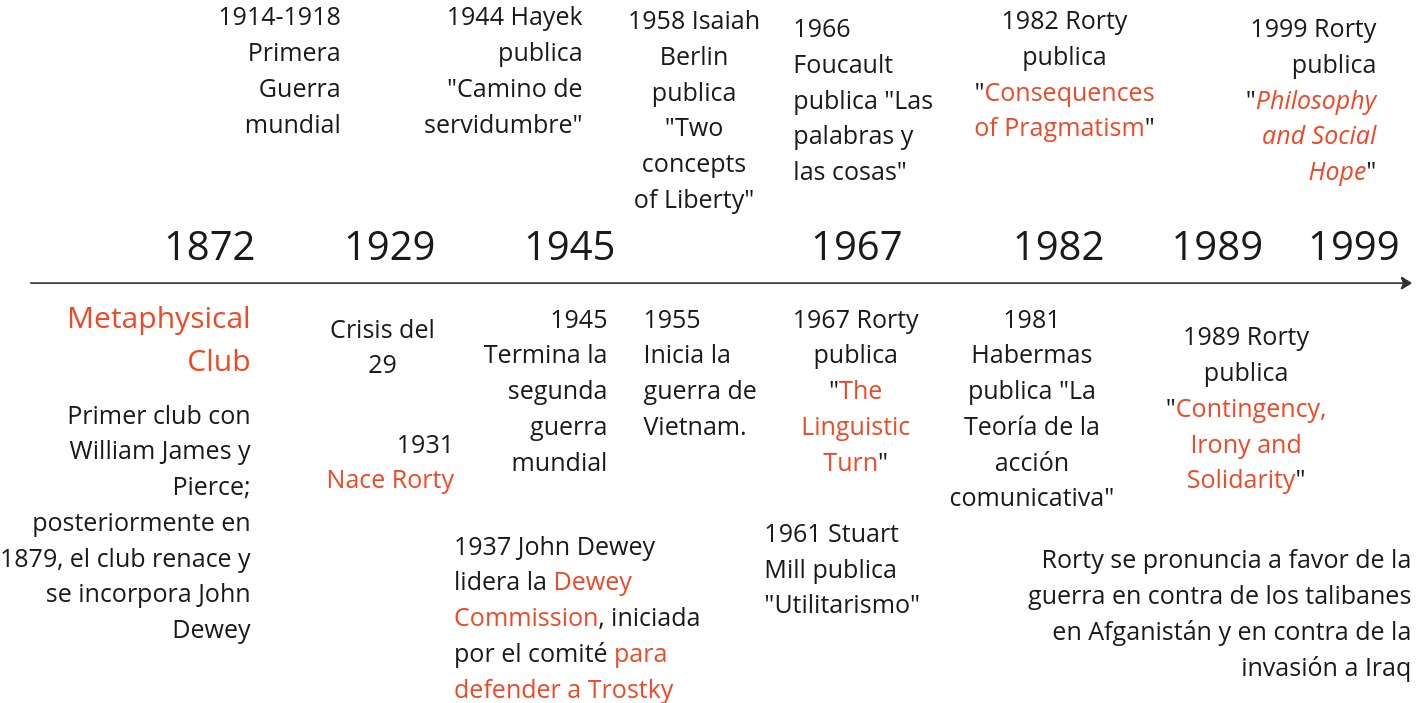
\includegraphics[keepaspectratio]{www/4_1_linea_tiempo_pragmatismo.jpg}}
\end{center}

\subsubsection{\texorpdfstring{Mapa Conceptual
(\citeproc{ref-stritzky2008}{Stritzky 2008}) -
(\citeproc{ref-belloreguera2018}{Bello Reguera
2018})}{Mapa Conceptual (Stritzky 2008) - (Bello Reguera 2018)}}\label{mapa-conceptual-stritzky2008---belloreguera2018}

\begin{center}
\pandocbounded{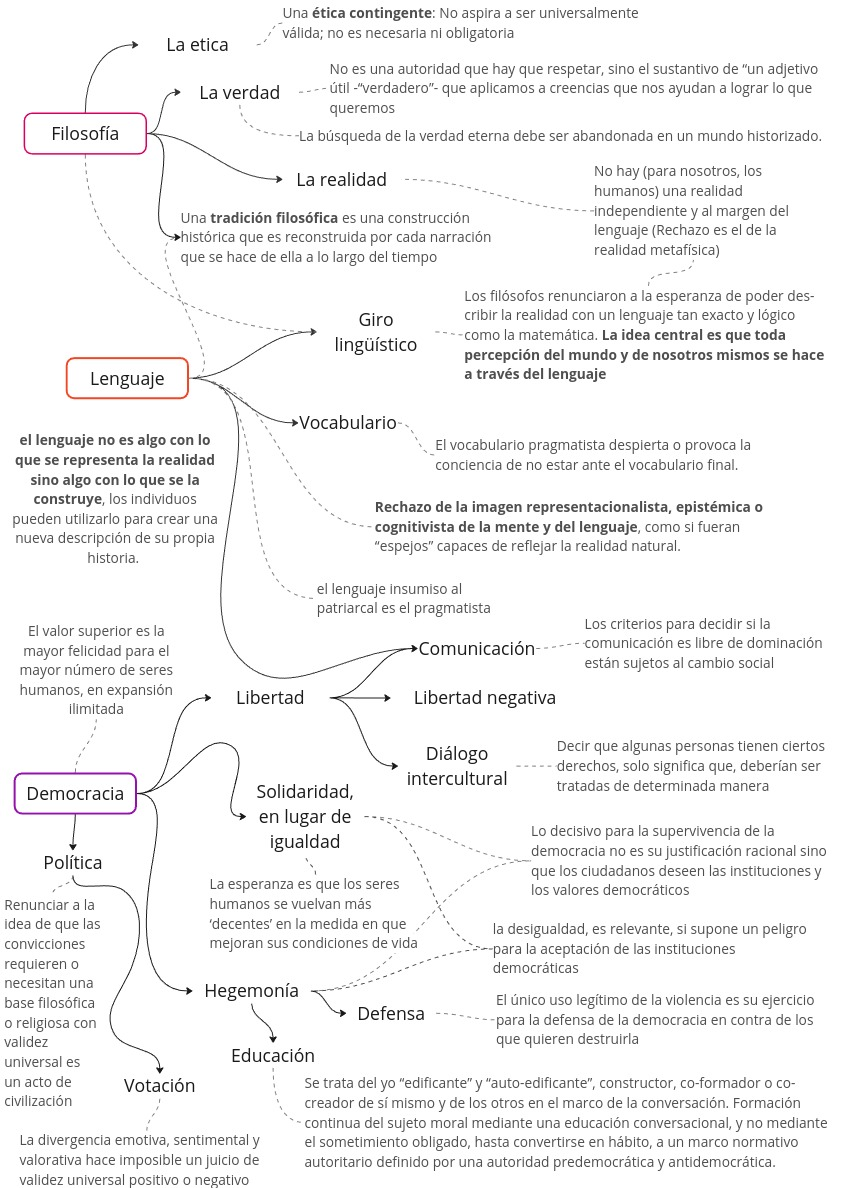
\includegraphics[keepaspectratio]{www/4_3_pragmatismo.jpg}}
\end{center}

\begin{center}
\pandocbounded{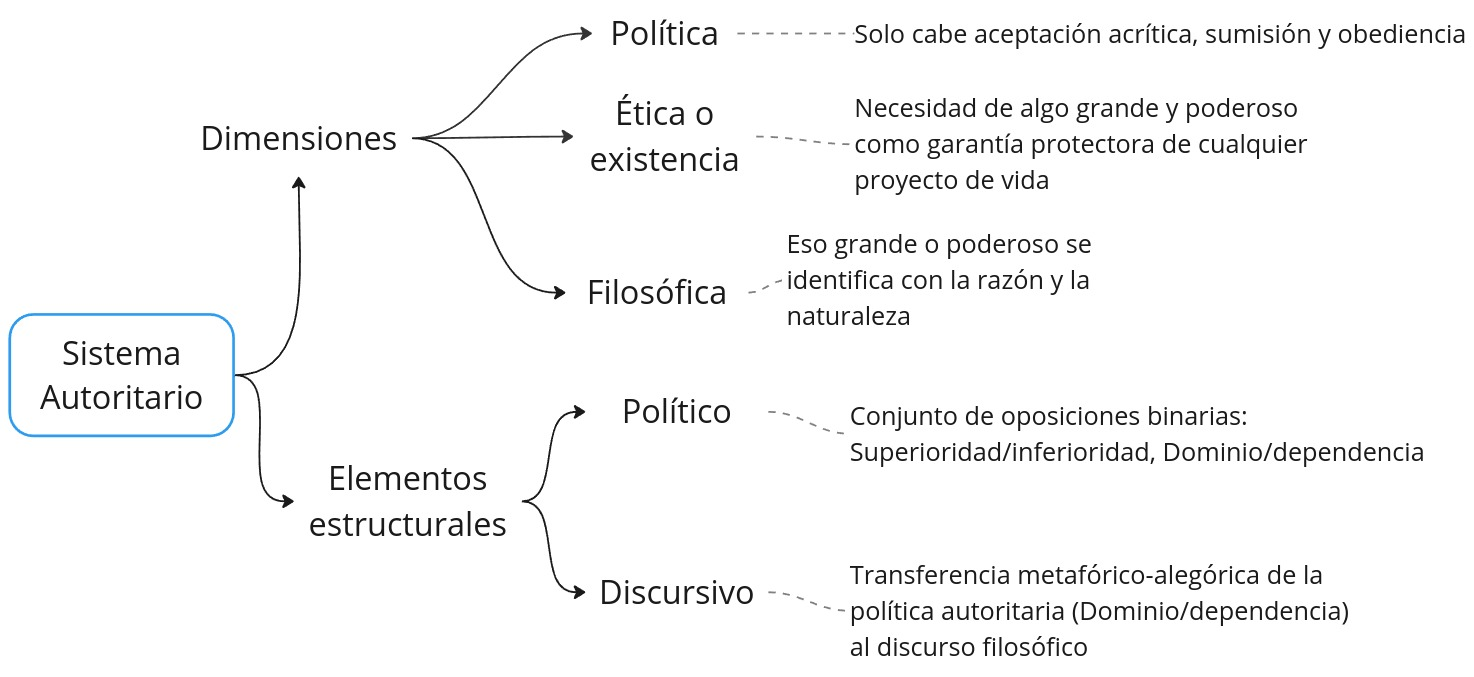
\includegraphics[keepaspectratio]{www/4_2_autoritarismo.jpg}}
\end{center}

\chapter{Libertad y republicanismo}\label{libertad-y-republicanismo}

\begin{longtable}[]{@{}
  >{\raggedright\arraybackslash}p{(\linewidth - 0\tabcolsep) * \real{1.0079}}@{}}
\toprule\noalign{}
\endhead
\bottomrule\noalign{}
\endlastfoot
\begin{minipage}[t]{\linewidth}\raggedright
\begin{itemize}
\item
  ``Las paradojas de la Libertad''. Quentin Skinner p 93-114
\item
  ``Liberalismo y Republicanismo''. Phillip Pettit p.115-135
\end{itemize}

Ovejero Féix, Martí, José Luis, y Gargarella, Roberto (Compiladores)
\textbf{Nuevas ideas republicanas. Autogobierno y Libertad}.
\end{minipage} \\
\end{longtable}

\section{Las paradojas de la
libertad}\label{las-paradojas-de-la-libertad}

\subsection{Libertad negativa}\label{libertad-negativa}

\begin{quote}
La libertad política es fundamentalmente negativa: ausencia de cierto
grado de coerción que le impida al agente ser capaz de actuar en pos de
sus propios fines, ser capaz de buscar distintas opciones, o al menos
ser capaz de elegir entre diversas alternativas. Isaiah Berlin.
\end{quote}

\begin{figure}

\caption{\label{fig-paradoja_libneg}}

\centering{

\pandocbounded{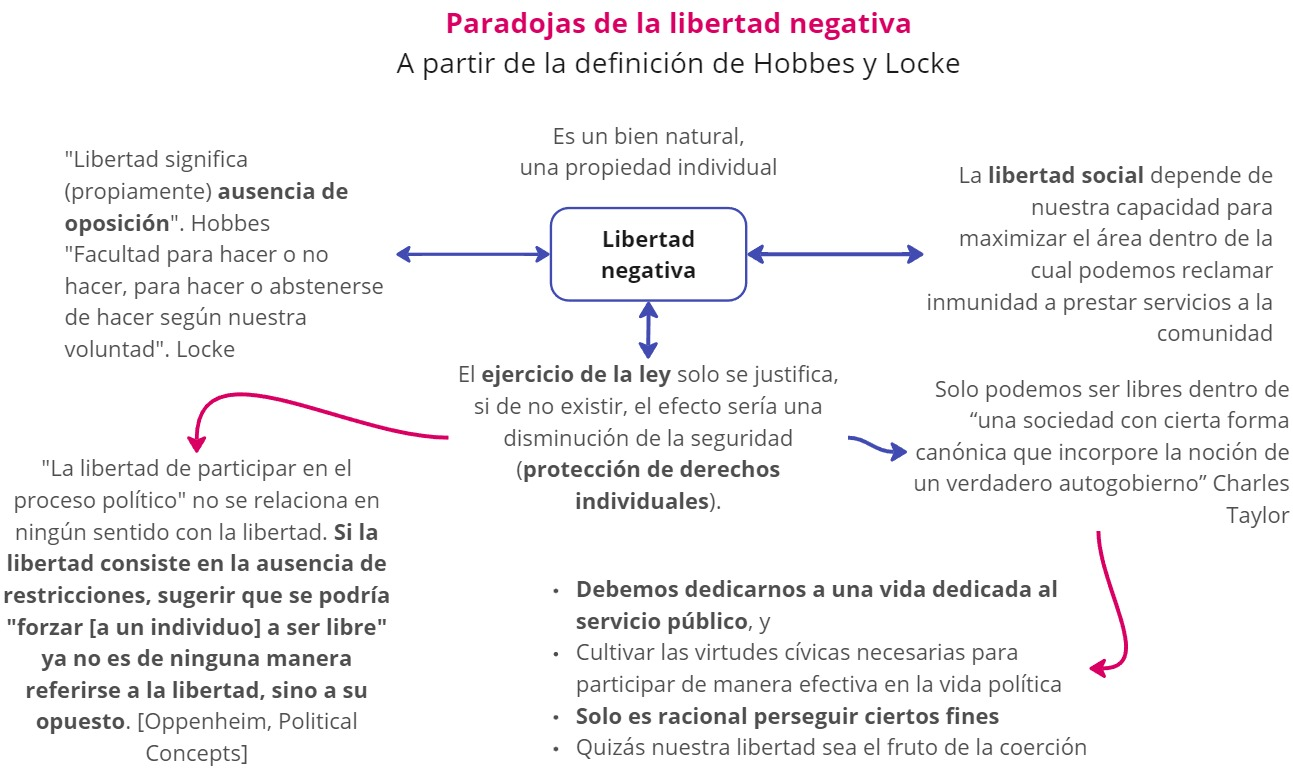
\includegraphics[keepaspectratio]{www/6_paradoja_libneg.jpg}}

}

\end{figure}%

\begin{itemize}
\item
  ``La libertad significa (propiamente) ausencia de oposición'' Hobbes,
  Leviatán.

  \begin{quote}
  ``La libertad es simple, consiste en la facultad para hacer o no
  hacer, para hacer o abstenerse de hacer según nuestra voluntad. Esto
  no se puede negar'' Locke
  \end{quote}

  \begin{itemize}
  \tightlist
  \item
    Para Hobbes y Locke la libertad es un bien natural, una propiedad
    individual; la exigencia de que el ejercicio de la ley solo se puede
    justificar si se demuestra que de no existir, el efecto no sería una
    libertad más amplia sino una disminución de la seguridad gracias a
    la cual se goza de libertad (protección de derechos individuales).
  \end{itemize}

  \begin{itemize}
  \item
    La maximización de nuestra libertad social debe depender de nuestra
    capacidad para maximizar el área dentro de la cual podemos reclamar
    inmunidad a prestar servicios a la comunidad.
  \item
    ``La libertad de participar en el proceso político'' no se relaciona
    en ningún sentido con la libertad. Si la libertad consiste en la
    ausencia de restricciones, sugerir que se podría ``forzar {[}a un
    individuo{]} a ser libre'' ya no es de ninguna manera referirse a la
    libertad, sino a su opuesto. {[}Oppenheim, Political Concepts{]}
  \end{itemize}
\item
  Solo podemos ser libres dentro de ``una sociedad con cierta forma
  canónica que incorpore la noción de un verdadero autogobierno''
  Charles Taylor

  Entonces

  \begin{itemize}
  \item
    debemos dedicarnos a una vida dedicada al servicio público, y
  \item
    cultivar las virtudes cívicas necesarias para participar de manera
    efectiva en la vida política
  \end{itemize}

  Solo es racional perseguir ciertos fines
\item
  Quizás nuestra libertad sea el fruto de la coerción
\end{itemize}

\subsection{Teoría positiva de la
libertad}\label{teoruxeda-positiva-de-la-libertad}

\begin{figure}

\caption{\label{fig-paradoja_libpos}}

\centering{

\pandocbounded{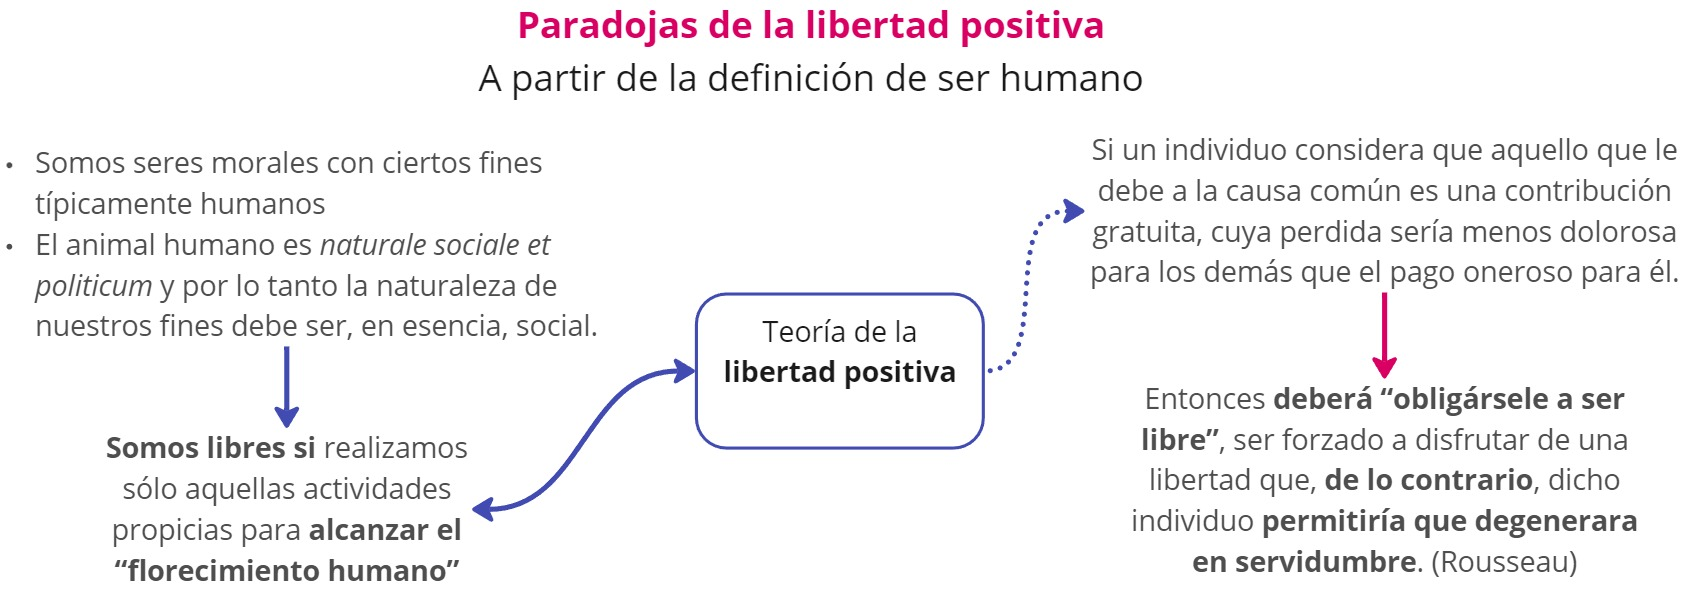
\includegraphics[keepaspectratio]{www/6_paradoja_libpos.jpg}}

}

\end{figure}%

\begin{itemize}
\item
  Somos seres morales con ciertos fines típicamente humanos
\item
  El animal humano es \emph{naturale sociale et politicum} y por lo
  tanto la naturaleza de nuestros fines debe ser, en esencia, social.

  \begin{itemize}
  \item
    Entonces somos libres si realizamos solo aquellas actividades
    propicias para alcanzar el ``florecimiento humano''.
  \item
    Si un individuo considera que aquello que le debe a la causa común
    es una contribución gratuita, cuya perdida sería menos dolorosa para
    los demás que el pago oneroso para él, entonces deberá ``obligársele
    a ser libre'', ser forzado a disfrutar de una libertad que, de lo
    contrario, dicho individuo permitiría que degenerara en servidumbre.
    (Rousseau)
  \end{itemize}
\end{itemize}

\subsection{Republicanismo clásico}\label{republicanismo-cluxe1sico}

\begin{figure}

\caption{\label{fig-repclas}}

\centering{

\pandocbounded{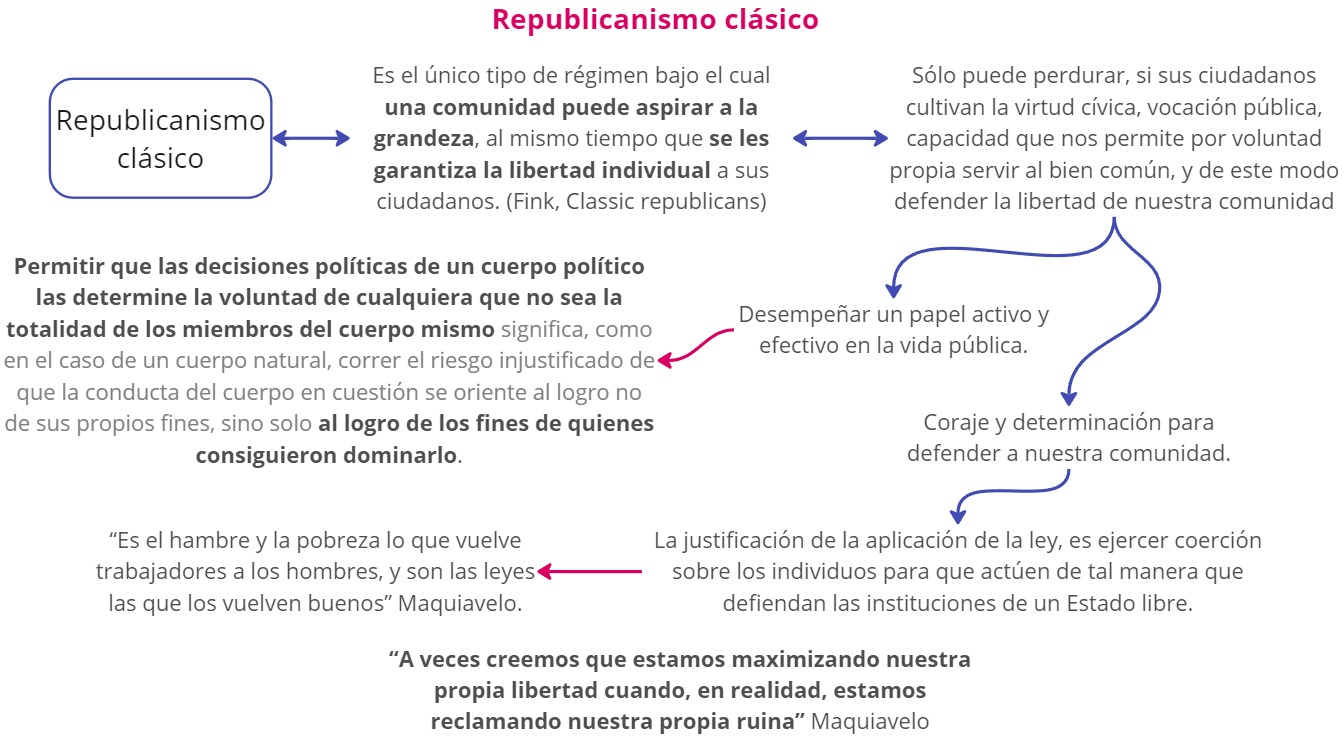
\includegraphics[keepaspectratio]{www/6_paradoja_repuclas.jpg}}

}

\end{figure}%

Una república que se autogobierna es el único tipo de régimen bajo el
cual una comunidad puede aspirar a la grandeza al mismo tiempo que les
garantiza a sus ciudadanos la libertad individual. (Fink, Classic
republicans).

\begin{itemize}
\item
  Una república que se autogobierna sólo puede perdurar, si sus
  ciudadanos cultivan la virtud cívica, vocación pública, capacidad que
  nos permite por voluntad propia servir al bien común, y de este modo
  defender la libertad de nuestra comunidad.

  \begin{itemize}
  \item
    Coraje y determinación para defender a nuestra comunidad.
  \item
    Desempeñar un papel activo y efectivo en la vida pública.
  \end{itemize}

  Permitir que las decisiones políticas de un cuerpo político las
  determine la voluntad de cualquiera que no sea la totalidad de los
  miembros del cuerpo mismo significa, como en el caso de un cuerpo
  natural, correr el riesgo injustificado de que la conducta del cuerpo
  en cuestión se oriente al logro no de sus propios fines, sino solo al
  logro de los fines de quienes consiguieron dominarlo.

  \begin{quote}
  ``A veces creemos que estamos maximizando nuestra propia libertad
  cuando, en realidad, estamos reclamando nuestra propia ruina''
  Maquiavelo

  ``Es el hambre y la pobreza lo que vuelve trabajadores a los hombres,
  y son las leyes las que los vuelven buenos'' Maquiavelo.

  La justificación de la aplicación de la ley, es ejercer coerción sobre
  los individuos para que actúen de tal manera que defiendan las
  instituciones de un Estado libre.
  \end{quote}
\end{itemize}

\section{Liberalismo y
republicanismo}\label{liberalismo-y-republicanismo}

\begin{figure}

\caption{\label{fig-6librep}}

\centering{

\pandocbounded{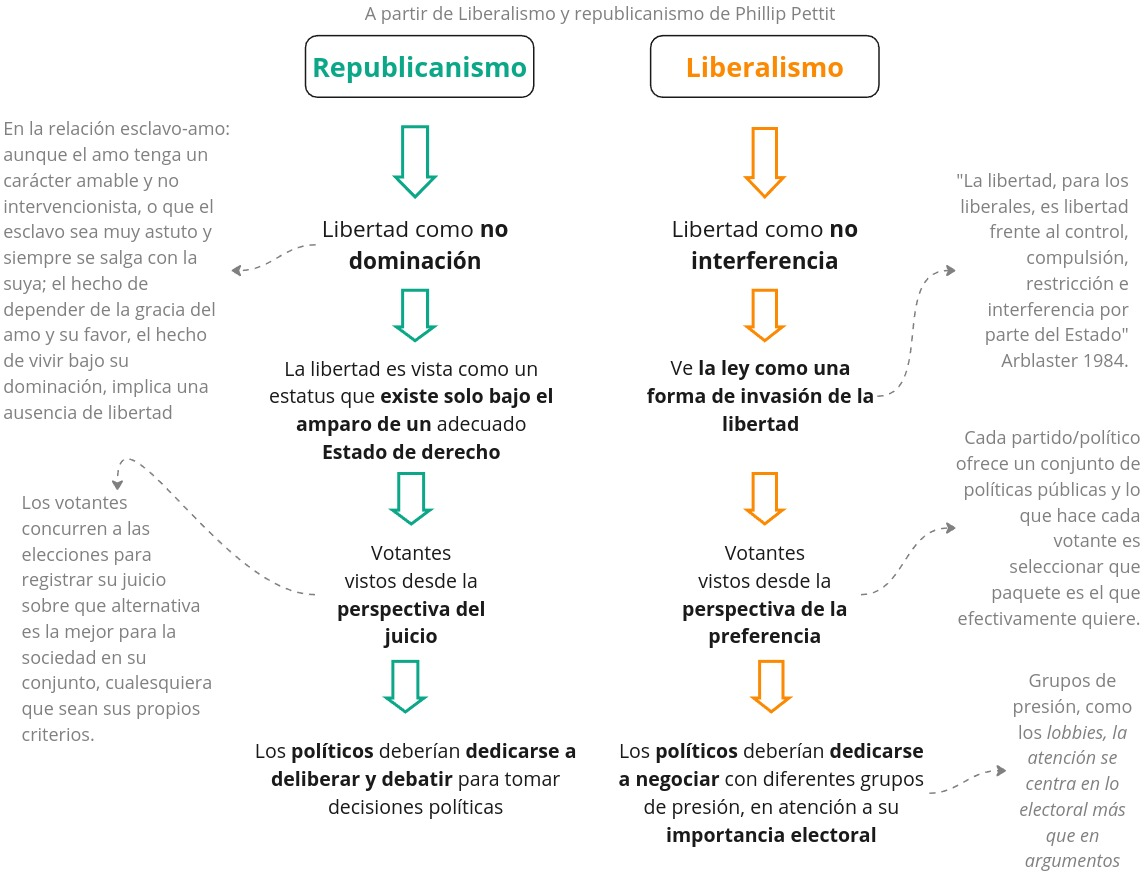
\includegraphics[keepaspectratio]{www/6_lib_rep.jpg}}

}

\end{figure}%

\begin{itemize}
\item
  Libertad

  \begin{quote}
  (republicanismo) Libertad como no dominación, ausencia de dominación.

  (liberalismo) Libertad como no interferencia: ausencia de
  interferencia.
  \end{quote}

  Ejemplo en la relación esclavo-amo: aunque el amo tenga un carácter
  amable y no intervencionista, o que el esclavo sea muy astuto y
  siempre se salga con la suya; el hecho de depender de la gracia del
  amo y su favor, el hecho de vivir bajo su dominación, implica una
  ausencia de libertad.

  Ejemplo en pago de impuestos: un individuo esta sujeto a coerción, por
  el estado de derecho, para pagar impuestos, pero no necesariamente
  esta sujeto a la voluntad arbitraria del Estado.

  \begin{quote}
  ``El hombre que no puede vivir por sí mismo debe ser un sirviente;
  pero aquel que puede vivir por sí mismo puede ser un hombre libre''
  Harrington

  ``Libertad es vivir de acuerdo con los términos de uno; esclavitud es
  vivir a merced de otro'' Treuchard y Gordon, 1971.
  \end{quote}
\item
  Ley

  \begin{itemize}
  \item
    (republicanismo) La libertad es vista como un estatus que existe
    solo bajo el amparo de un adecuado Estado de derecho.
  \item
    (liberalismo) Ve la ley como una forma de invasión de la libertad
    del pueblo. ``La libertad, para los liberales, es libertad frente al
    control, compulsión, restricción e interferencia por parte del
    Estado'' Arblaster 1984.
  \end{itemize}
\item
  Votantes

  \begin{itemize}
  \item
    (republicanismo) Perspectiva del juicio:

    \begin{itemize}
    \tightlist
    \item
      Los votantes concurren a las elecciones para registrar su juicio
      sobre que alternativa es la mejor para la sociedad en su conjunto,
      cualesquiera que sean sus propios criterios.
    \end{itemize}
  \item
    (liberalismo) Perspectiva de preferencias:

    \begin{itemize}
    \tightlist
    \item
      Cada partido/político ofrece un conjunto de políticas públicas y
      lo que hace cada votante es seleccionar que paquete es el que
      efectivamente quiere.
    \end{itemize}
  \end{itemize}
\item
  Políticos

  \begin{itemize}
  \item
    (republicanismo) Los políticos deberían dedicarse a deliberar y
    debatir para tomar decisiones políticas.
  \item
    (liberalismo) Los políticos deberían dedicarse a negociar con
    diferentes grupos de presión, en atención a su importancia electoral
    y no en atención a sus argumentos.
  \end{itemize}
\end{itemize}

\chapter{La Clase Política}\label{clase_pol}

\begin{quote}
Reporte de lectura:

``La Clase Política'' (\citeproc{ref-mosca1992}{Mosca 1992})\footnote{Ed.
  original: G. Mosca, Elementi di Scienza Politica, cap. 2, La terza,
  Roma, 1896.}, incluido en el libro ``Diez textos básicos de ciencia
política'' (\citeproc{ref-rubio1992}{Rubio 1992}).
\end{quote}

\section{Síntesis}\label{suxedntesis}

Mosca sustenta que, en todas las sociedades, sin importar su forma de
gobierno, o que tan avanzadas sean, existe una minoría organizada
llamada \emph{clase política}; la cual gobierna sobre una mayoría
desorganizada. Las minorías gobernantes, desempeñan todas las funciones
políticas, monopolizan el poder y disfrutan de las ventajas que van
unidas a él; además están constituidas de tal manera que los individuos
que las componen se distinguen de los gobernados por algunas cualidades
que les otorgan cierta superioridad material, intelectual, religiosa o
moral; verdadera o aparente, que es muy apreciada y se valora mucho en
la sociedad en que viven; o bien que son los herederos de quienes tenían
esas cualidades.

\section{Tesis}\label{tesis}

Toda sociedad, desde la más primitiva hasta la más avanzada, esta
dividida en dos clases: una minoría gobernante y una mayoría gobernada.
La primera, denominada \emph{clase política}, se encuentra organizada y
desempeña todas las funciones políticas, ostenta el monopolio del poder
y de sus ventajas; además, posibilita a sus miembros el aprendizaje del
arte de gobernar. La segunda estará desorganizada por cuanto que no
posee el poder; lo que es el objeto del dominio; los hábitos de
obediencia inculcados por los gobernantes les impedirán acceder a la
pericia política.

\section{Ideas secundarías}\label{ideas-secundaruxedas}

\begin{itemize}
\item
  Si los individuos que conforman la clase política desaparecen, se
  constituiría rápidamente otro grupo de individuos organizados que
  pasaría a desempeñar la función de dicha clase.
\item
  Entre más grande y complejo sea un Estado, más favorable serán las
  condiciones para la dominación de una minoría y; por el contrario,
  entre más pequeño y simple sea, mayor será la probabilidad de
  organización, control y respuesta de la clase gobernada.
\item
  Todas las clases políticas tienden a volverse hereditarias, si no de
  derecho, al menos de hecho. La fuerza, la riqueza y el saber son el
  puente que sirve de medio para trasmitir el poder; pero estos
  elementos no trasmiten la capacidad teórica y práctica de la política;
  la herencia más rica es la posesión del mando: el legado del poder es
  lo más valioso.
\end{itemize}

\section{Reflexión}\label{reflexiuxf3n}

La \emph{teoría de las élites,} que se fundamentó sobre los trabajos de
(\citeproc{ref-mosca1992}{Mosca 1992}),
(\citeproc{ref-michels2010}{Michels 2010}) y
(\citeproc{ref-pareto1916}{Pareto 1916}), establece la inevitabilidad de
una dicotomía, élite-masa, en la sociedad; una minoría gobernante y una
mayoría gobernada. Plantea que la existencia de la minoría gobernante es
una necesidad funcional de cualquier sociedad compleja, donde la
especialización, la burocracia y la necesidad de liderazgo hacen que el
poder se concentre en pocos individuos; no obstante, la composición de
esta élite no es estática, se renueva o reemplaza constantemente, ya sea
de forma gradual (por la cooptación de nuevos miembros) o abrupta (a
través de revoluciones).

La élite gobernante, de acuerdo con (\citeproc{ref-mills1956}{Mills
1956}), no es solo la clase política, sino que es un triunvirato
compuesto por las élites política, económica y militar; además
considerando el trabajo de Bourdieu (\citeproc{ref-huang2019}{Huang
2019}), se podría incluir a la élite cultural; aunque propiamente él
hablaba de que existen cuatro formas de capital que se retroalimentan
entre sí, el capital económico, social, cultural y simbólico.

\subsection{Élites en México}\label{uxe9lites-en-muxe9xico}

En el caso de México, la narrativa usual es la legitimación de las
élites por medio de la meritocracia, respaldando la interpretación de
que la posición que ocupan y su pertenencia a esa élite es debido a lo
que han alcanzado o hecho por mérito individual y no por el contexto en
el que nacieron o en el que se desenvuelven. Mosca señalaba que los
individuos pertenecientes a las aristocracias sustentaban sus cualidades
especiales, no tanto a la sangre que corría por sus venas, como a la
esmerada educación que habían recibido y que había desarrollado en ellos
ciertas tendencias intelectuales y morales con preferencia a otras.

En México, desde la revolución mexicana, de acuerdo con Behrend
(\citeproc{ref-behrend2021}{Behrend 2021}), surgió un grupo de lideres
pertenecientes a la \emph{familia revolucionaria}, que ejercieron el
poder político en México varios años después de la lucha revolucionaria
a través del movimiento que llegaría a ser el Partido Revolucionario
Institucional, PRI. Schmidt y Mendieta
(\citeproc{ref-schmidt2002}{Schmidt y Mendieta 2002}) señalan que la red
de poder inició una bifurcación en los años cuarenta, separando a los
políticos y a los financieros; en este tenor es posible que a partir de
la llegada a la presidencia del partido Movimiento de Regeneración
Nacional, Morena, se haya generado otra bifurcación en la red de poder
en México.

\section{Contexto histórico en el que vivió Gaetano Mosca
(1858-1941)}\label{contexto-histuxf3rico-en-el-que-viviuxf3-gaetano-mosca-1858-1941}

\begin{center}
\pandocbounded{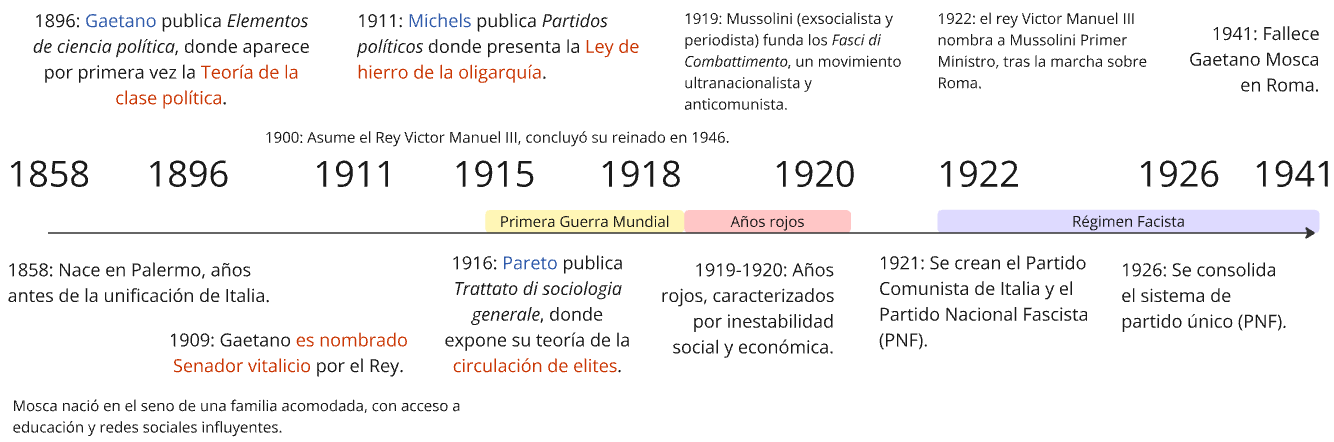
\includegraphics[keepaspectratio]{www/07_ClasePolitica.png}}
\end{center}

\chapter{La poliarquía}\label{poliarquia}

\begin{quote}
Reporte de lectura:

Dahl, Robert Alan. «La poliarquía.» En \emph{Diez textos básicos de
ciencia política}, de Albert Batlle Rubio, 77-92. Barcelona, España:
Ariel, 1992.

* Ed. original: R. A. Dahl, \emph{A Preface to Democratic Theory}, cap.
3, The University of Chicago Press, 1956.
\end{quote}

\section{Síntesis}\label{suxedntesis-1}

Dahl plantea que la democracia es una utopía, un ideal que los estados,
que se denominan democráticos, aspiran a alcanzar; un ideal donde hay
perfecta igualdad política y soberanía popular; por lo que sostiene que
en la práctica los estados ``democráticos'' tienden a ser regímenes
poliárquicos. La definición de estos regímenes la desarrolla al buscar
maximizar el \emph{gobierno del pueblo} (soberanía popular e igualdad
política), lo que resulta en el establecimiento de ocho condiciones que
podrían ser vistas como una definición operativa de democracia.

\section{Tesis}\label{tesis-1}

Al presuponer que la democracia, en su definición teórica, es una
utopía, Dahl plantea las siguientes condiciones que se deberían alcanzar
para, en la realidad, tratar de lograr un gobierno del pueblo:

\begin{enumerate}
\def\labelenumi{\arabic{enumi}.}
\item
  Derecho a la expresión de preferencias (p.e. derecho al voto).
\item
  El peso de la elección de cada individuo es idéntico.
\item
  La alternativa más seleccionada es la ganadora.
\item
  Cualquiera que perciba un conjunto de alternativas, y considere al
  menos una de ellas preferible a las demás, puede añadirla a las
  seleccionadas para la votación.
\item
  Todos poseen idéntica información sobre las alternativas.
\item
  Las alternativas con más votos desplazan a las que tienen menos votos.
\item
  Las ordenes de los cargos electos se cumplen.
\item
  Las nuevas decisiones del período interelectoral están regidas por las
  condiciones precedentes; o que las decisiones interelectorales están
  subordinadas a las establecidas durante la etapa de elección o que son
  aplicación de éstas.
\end{enumerate}

\section{Ideas secundarías}\label{ideas-secundaruxedas-1}

\begin{itemize}
\item
  La poliarquía no es ni un gobierno de mayoría pura ni un gobierno
  unificado de una minoría. Es un sistema abierto, competitivo y
  pluralista de gobierno de minorías.
\item
  El nivel de poliarquía existente dependerá de la medida en que se
  consideren deseables las ocho condiciones.
\item
  La poliarquía es una función de la actividad política de los miembros.
\item
  El nivel de instrucción social en una de las ocho condiciones aumenta
  también con el grado de acuerdo existente sobre ella.
\end{itemize}

\section{Reflexión}\label{reflexiuxf3n-1}

Leyendo el texto de Dahl desde la perspectiva de la teoría de la clase
política de Mosca, pareciera que ``la poliarquía es una negociación
entre minorías organizadas'' (\citeproc{ref-krouse1982}{Krouse 1982})
inmersas en una mayoría desorganizada, dando pie a un ``juego
democrático'' (\citeproc{ref-bovero1998}{Bovero 1998}) que busca
maximizar el consenso y minimizar la imposición bajo las reglas
democráticas; donde la ``efectividad política de cada grupo estaría en
función de su potencial de control y de unidad''
(\citeproc{ref-dahl1958}{Dahl 1958}).

Desde un punto de vista práctico, la propuesta de Dahl puede brindar una
escala medible para ver qué tan cerca un estado o institución se
encuentra de ser democrático (poliárquico); y, aunque las condiciones o
normas planteadas no dan de manera operativa un camino para alcanzar la
democracia, en su definición ideal, sí permiten plantear objetivos
reales para acercarse a estados más democráticos.

Actualmente, El Economista plantea un índice
(\citeproc{ref-theeconomistintelligenceunit2025}{The Economist
Intelligence Unit 2025}), que mide la democracia de los países usando
cinco categorías: Libertades civiles, Participación Política, Proceso
electoral y pluralismo, Funcionamiento del gobierno y Cultura política;
de acuerdo con los resultados, clasifica a los países en cuatro
categorías que van de Democracias completas a Regímenes autoritarios. En
2024, ubicó a México como un régimen Hibrido, además ha mantenido una
tendencia a la baja desde 2013, ver Figura~\ref{fig-democracyindex} . La
IDEA, por su parte, plantea cuatro índices para medir el estado de la
democracia
(\citeproc{ref-internationalinstitutefordemocracyandelectoralassistance2025}{Democracy
y Electoral Assistance 2025}): Representación, Derechos, Participación y
Estado de Derecho; en 2024 resaltó que el índice que México tiene más
bajo es el de Estado de Derecho, con 0.36 en una escala de 0-1; debido a
que este índice tiene un subíndice que mide la independencia del poder
judicial.

\begin{figure}

\caption{\label{fig-democracyindex}Índice de la democracia en México.}

\centering{

\pandocbounded{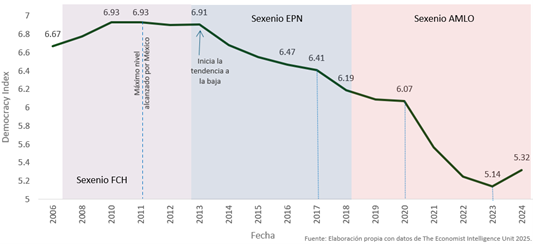
\includegraphics[keepaspectratio]{www/08_poliarquia.png}}

}

\end{figure}%

\chapter{Ingeniería social}\label{ing_social}

\section{Teóricos y defensores de la ingeniería
social}\label{teuxf3ricos-y-defensores-de-la-ingenieruxeda-social}

Creían que el conocimiento científico podía y debía ser usado para
planificar y mejorar racionalmente la sociedad.

\subsection{Utopistas y Positivistas}\label{utopistas-y-positivistas}

\begin{itemize}
\tightlist
\item
  \textbf{Auguste Comte} (1798-1857): Quizás el primer gran teórico,
  creía que el estudio científico de la sociedad (la ``física social'' o
  \textbf{sociología}) permitiría descubrir sus leyes y, por lo tanto,
  dirigir la sociedad racionalmente hacia el orden y el progreso,
  reemplazando a la religión. Los gobernantes deberían ser
  ``sacerdotes'' de la ciencia social.
\item
  \textbf{Karl Marx} (1818-1883) \textbf{y Friedrich Engels}
  (1820-1895): Aunque no usaron el término, su teoría es un tipo de
  ingeniería social macro. Postularon que mediante la
  \textbf{revolución} y la \textbf{dictadura del proletariado}, se
  podría derrumbar la sociedad capitalista y construir conscientemente
  una sociedad comunista, libre de clases. La planificación económica
  central es una forma extrema de ingeniería social.
\item
  \textbf{Los Socialistas Utopistas} (Saint-Simon, Charles Fourier,
  Robert Owen)\textbf{:} Predecesores de Marx, diseñaron comunidades
  modelo perfectas en el papel, creyendo que podían recrearlas en la
  realidad mediante un diseño racional.
\end{itemize}

\subsection{Los pragmáticos y reformistas
liberales-progresistas}\label{los-pragmuxe1ticos-y-reformistas-liberales-progresistas}

\begin{itemize}
\tightlist
\item
  \textbf{Jeremy Bentham} (1748-1832) y los \textbf{Utilitaristas:} Su
  principio de ``\textbf{la mayor felicidad para el mayor número}'' es
  el motor filosófico de mucha ingeniería social. Si se puede medir la
  felicidad, se pueden diseñar políticas e instituciones (como su famoso
  \textbf{Panóptico}) para maximizarla. El estado es un ingeniero de la
  felicidad pública.
\item
  \textbf{Los Fabianos} (Sociedad Fabiana, fundada en 1884 - Reino
  Unido): Think tank clave que influyó en el Partido Laborista. Abogaban
  por un \textbf{socialismo gradualista} y reformista, logrado no por
  revolución, sino mediante la ``\textbf{permeación}'' de las
  instituciones existentes. Creían en la planificación estatal y la
  expertise técnica para dirigir la economía y la sociedad (ejemplos:
  George Bernard Shaw, Sidney y Beatrice Webb).
\item
  \textbf{John Dewey} (1859-1952): Filósofo pragmático estadounidense.
  Veía la educación no como la transmisión de conocimiento estático,
  sino como la herramienta principal para \textbf{construir una sociedad
  democrática y adaptada a los tiempos}. La escuela era el laboratorio
  para la ingeniería social democrática.
\end{itemize}

\subsection{Planificación Central}\label{planificaciuxf3n-central}

\begin{itemize}
\tightlist
\item
  \textbf{Vladimir Lenin} (1870-1924) y los \textbf{Bolcheviques:}
  Llevaron la teoría marxista a la práctica, usando el estado de manera
  coercitiva para remodelar por completo la sociedad rusa, la economía e
  incluso la cultura y la moral (``\textbf{Hombre Soviético Nuevo}'').
\item
  \textbf{Tecnócratas y Planificadores Económicos:} Figuras como
  \textbf{John Maynard Keynes} (1883-1946), aunque no era un ingeniero
  social radical, defendió la \textbf{intervención estatal en la
  economía} (fiscal y monetaria) para suavizar los ciclos económicos y
  lograr el pleno empleo. Esto es una forma de ``ingeniería económica
  macro''.
\end{itemize}

\section{Críticos: visión negativa o de
advertencia}\label{cruxedticos-visiuxf3n-negativa-o-de-advertencia}

Estos pensadores vieron en la ingeniería social la arrogancia del
racionalismo y una amenaza directa a la libertad individual y a la
evolución social espontánea.

\subsection{Liberales clásicos y
conservadores}\label{liberales-cluxe1sicos-y-conservadores}

\begin{itemize}
\tightlist
\item
  \textbf{Friedrich Hayek} (1899-1992): Su obra maestra,
  \textbf{``Camino de Servidumbre''} (1944), es la crítica más famosa.
  Argumenta que toda planificación central conduce inevitablemente a la
  tiranía. La sociedad es demasiado compleja para que cualquier mente o
  grupo la comprenda y dirija. La ingeniería social, al querer imponer
  un diseño racional, ignora el \textbf{conocimiento tácito y disperso}
  que poseen los individuos y sofoca la libertad.
\item
  \textbf{Karl Popper} (1902-1994): En su libro \textbf{``La Sociedad
  Abierta y Sus Enemigos''} (1945), ataca a Platón, Hegel y Marx como
  profetas de un historicismo que justifica la ingeniería social a gran
  escala. Popper defiende en su lugar la \textbf{``ingeniería social
  gradualista o fragmentaria''}, que busca resolver problemas concretos
  mediante prueba y error, en lugar de intentar remodelar la sociedad
  entera según un plan utópico.
\item
  \textbf{Michael Oakeshott} (1901-1990): Filósofo político conservador
  británico. Criticaba la racionalidad en política, defendiendo que la
  sociedad no es una empresa que pueda ser dirigida hacia un fin
  específico, sino una conversación continua cuyas tradiciones y
  prácticas no pueden ser ``diseñadas'' desde cero.
\end{itemize}

\subsection{Los Disidentes del
Totalitarismo}\label{los-disidentes-del-totalitarismo}

\begin{itemize}
\tightlist
\item
  \textbf{Aleksandr Solzhenitsyn} (1918-2008): A través de su literatura
  (``\textbf{Archipiélago Gulag}''), expuso los horrores concretos de la
  ingeniería social aplicada en la Unión Soviética. Mostró cómo el
  intento de crear un ``hombre nuevo'' requería la destrucción de
  millones de hombres reales.
\end{itemize}

\section{Resumen}\label{resumen}

\begin{longtable}[]{@{}
  >{\raggedright\arraybackslash}p{(\linewidth - 6\tabcolsep) * \real{0.2500}}
  >{\raggedright\arraybackslash}p{(\linewidth - 6\tabcolsep) * \real{0.2500}}
  >{\raggedright\arraybackslash}p{(\linewidth - 6\tabcolsep) * \real{0.2500}}
  >{\raggedright\arraybackslash}p{(\linewidth - 6\tabcolsep) * \real{0.2500}}@{}}
\toprule\noalign{}
\begin{minipage}[b]{\linewidth}\raggedright
Teórico
\end{minipage} & \begin{minipage}[b]{\linewidth}\raggedright
Corriente
\end{minipage} & \begin{minipage}[b]{\linewidth}\raggedright
Postura ante la Ingeniería Social
\end{minipage} & \begin{minipage}[b]{\linewidth}\raggedright
Obra Representativa
\end{minipage} \\
\midrule\noalign{}
\endhead
\bottomrule\noalign{}
\endlastfoot
Auguste Comte & Positivismo & Defensor & La sociedad debe ser dirigida
por una ``ciencia social''. \\
Karl Marx & Socialismo Científico & Defensor (revolucionario) & La
revolución es la ingeniería para una nueva sociedad. \\
Jeremy Bentham & Utilitarismo & Defensor (pragmático) & El estado debe
maximizar la felicidad mediante diseño. \\
Fabianos & Socialismo Gradualista & Defensores (reformistas) & Permear
el estado para una transición planificada al socialismo. \\
Friedrich Hayek & Liberalismo Clásico & Crítico Feroz & La planificación
central conduce a la tiranía. \\
Karl Popper & Racionalismo Crítico & Crítico (propone alternativa) &
Rechaza la ingeniería utópica, acepta la gradual. \\
\end{longtable}

El debate sobre la ingeniería social es, en el fondo, el debate eterno
entre \textbf{la libertad individual y la planificación colectiva},
entre el \textbf{racionalismo constructivista} y el \textbf{respeto por
el orden espontáneo}.

\part{Ciencias Sociales}

En construcción\ldots{}

\chapter{La noción de totalidad en las ciencias
sociales}\label{la-nociuxf3n-de-totalidad-en-las-ciencias-sociales}

\begin{quote}
Apuntes del artículo ``La noción de totalidad en las ciencias sociales''
(\citeproc{ref-lefebvre2011}{Lefebvre y Vargas 2011}).
\end{quote}

En Feuerbach el hombre completo y total reaparece más bien como dado
naturalmente que como reivindicación ética y social. El hombre total
existe en nosotros, en cada uno de nosotros naturalmente. A la vez,
totalidad y parte integrando la naturaleza, el hombre tiene según
Feuerbach los órganos precisos y necesarios para asir el universo en su
totalidad. Entre estos órganos figuran los sentidos, el su sexo, el
cerebro y el pensamiento.

Con Hegel, la noción de Totalidad se reencuentra con la contradicción
interna puesta en evidencia por los marxistas: a veces noción abierta,
cambiante, dialéctica -- a veces noción cerrada, sistémica,
metafísicamente impuesta desde afuera y separada del contenido viviente
del pensamiento hegeliano.

\begin{itemize}
\item
  \emph{Ningún fenómeno contiene por sí mismo a la totalidad absoluta de
  la realidad.} Es preciso superar dialécticamente sus sentidos formal y
  lógico: todo no está en todo --y cada ``todo'' es complejo,
  contradictorio. Cada totalidad (dispersa, cambiante, parcial) exige un
  análisis específico, aunque ligado a la metodología dialéctica
  general. De tal suerte que la noción de Totalidad solo se revela
  fecundamente a aquel que la considera dialécticamente.
\item
  \emph{El análisis económico-social alcanza las determinaciones
  esenciales, pero no las agota.} Así, yo observo esta mujer que compra
  azúcar, este hombre en un café. Para comprenderlos, me acerco a toda
  sociedad actual, a toda su historia. Descubro una confusa mezcla de
  causas y efectos, de acciones recíprocas, de ``esferas'', de esencias
  ocultas: la vida de este hombre o de esta mujer, su oficio, su
  familia, su nivel social, su clase, su biografía, etc\ldots. Así pues,
  también la ``estructura global'' del capitalismo. Pero el pequeño
  hecho inicial aparece como aún más rico y complejo,en su humildad, que
  las esencias, y las leyes y las profundidades implicadas.
\item
  La noción de totalidad aparece en las obras del joven Marx, de una
  manera profundamente original: en la noción de que él toma de
  Feuerbach, hombre total pero profundizada y transformada. El individuo
  es social, sin que se tenga el derecho de fijarlo, por el pensamiento,
  a la Sociedad en una abstracción exterior a él. Ni la naturaleza y la
  vida biológica, ni la vida de la especie humana y su historia, ni la
  vida individual y la vida social, no pueden separarse. El hombre es
  totalidad. Por sus necesidades y sus órganos, por sus sentidos y sus
  manos, por su trabajo, por la que lo transforma transformando el
  mundo, el hombre se apropia to praxis totalmente de la naturaleza
  entera y de su propia naturaleza. \emph{``El hombre se apropia de su
  ser universal de manera universal, pues en tanto hombre total''}
  (Manuscrits de 1844).
\item
\end{itemize}

\chapter{El mundo de la pseudoconcreción y su
destrucción}\label{el-mundo-de-la-pseudoconcreciuxf3n-y-su-destrucciuxf3n}

\begin{quote}
``Dialéctica de lo concreto'' (\citeproc{ref-karelkosuxedk1967}{Karel
Kosík 1967}).
\end{quote}

\pandocbounded{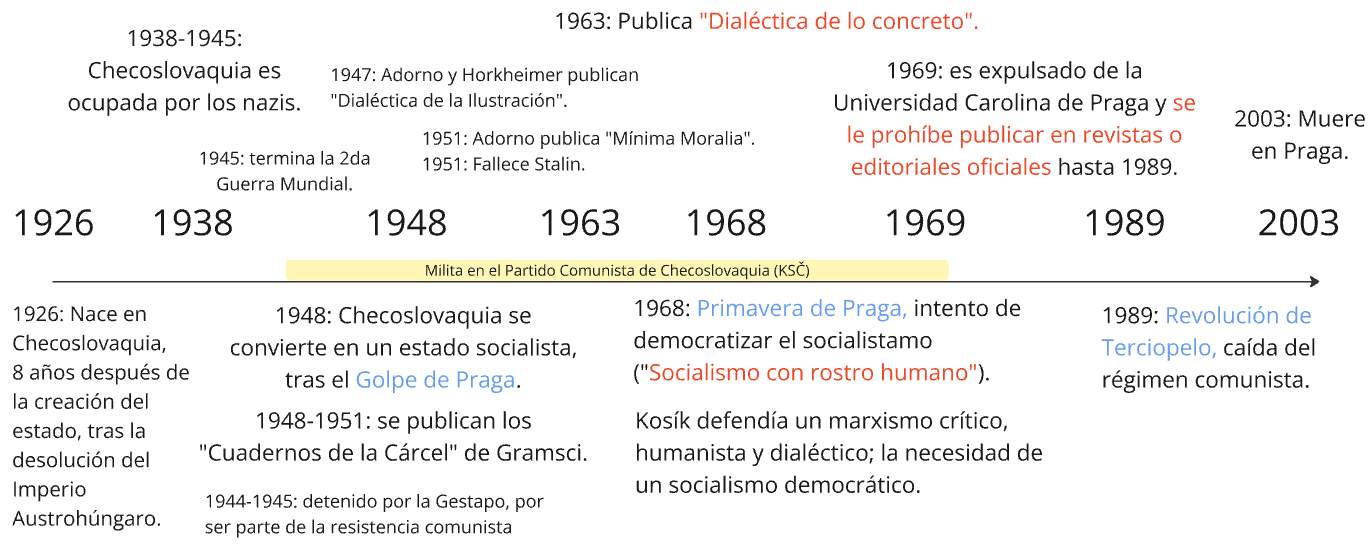
\includegraphics[keepaspectratio]{www/12_1_DialConcreto_.png}}

En Feuerbach el hombre completo y total reaparece más bien como dado
naturalmente que como reivindicación ética y social. El hombre total
existe en nosotros, en cada uno de nosotros naturalmente. A la vez,
totalidad y parte integrando la naturaleza, el hombre tiene según
Feuerbach los órganos precisos y necesarios para asir el universo en su
totalidad. Entre estos órganos figuran los sentidos, el su sexo, el
cerebro y el pensamiento.

Con Hegel, la noción de Totalidad se reencuentra con la contradicción
interna puesta en evidencia por los marxistas: a veces noción abierta,
cambiante, dialéctica -- a veces noción cerrada, sistémica,
metafísicamente impuesta desde afuera y separada del contenido viviente
del pensamiento hegeliano.

\begin{itemize}
\item
  \emph{Ningún fenómeno contiene por sí mismo a la totalidad absoluta de
  la realidad.} Es preciso superar dialécticamente sus sentidos formal y
  lógico: todo no está en todo --y cada ``todo'' es complejo,
  contradictorio. Cada totalidad (dispersa, cambiante, parcial) exige un
  análisis específico, aunque ligado a la metodología dialéctica
  general. De tal suerte que la noción de Totalidad solo se revela
  fecundamente a aquel que la considera dialécticamente.
\item
  \emph{El análisis económico-social alcanza las determinaciones
  esenciales, pero no las agota.} Así, yo observo esta mujer que compra
  azúcar, este hombre en un café. Para comprenderlos, me acerco a toda
  sociedad actual, a toda su historia. Descubro una confusa mezcla de
  causas y efectos, de acciones recíprocas, de ``esferas'', de esencias
  ocultas: la vida de este hombre o de esta mujer, su oficio, su
  familia, su nivel social, su clase, su biografía, etc\ldots. Así pues,
  también la ``estructura global'' del capitalismo. Pero el pequeño
  hecho inicial aparece como aún más rico y complejo,en su humildad, que
  las esencias, y las leyes y las profundidades implicadas.
\item
  La noción de totalidad aparece en las obras del joven Marx, de una
  manera profundamente original: en la noción de que él toma de
  Feuerbach, hombre total pero profundizada y transformada. El individuo
  es social, sin que se tenga el derecho de fijarlo, por el pensamiento,
  a la Sociedad en una abstracción exterior a él. Ni la naturaleza y la
  vida biológica, ni la vida de la especie humana y su historia, ni la
  vida individual y la vida social, no pueden separarse. El hombre es
  totalidad. Por sus necesidades y sus órganos, por sus sentidos y sus
  manos, por su trabajo, por la que lo transforma transformando el
  mundo, el hombre se apropia to praxis totalmente de la naturaleza
  entera y de su propia naturaleza. \emph{``El hombre se apropia de su
  ser universal de manera universal, pues en tanto hombre total''}
  (Manuscrits de 1844).
\end{itemize}

\chapter{Karel Kosík: Dialéctica de lo
concreto}\label{karel-kosuxedk-dialuxe9ctica-de-lo-concreto}

\section{Prologo}\label{prologo}

Karel Kosík es un joven filósofo checo, nacido en Praga en 1926. Como
militante del Partido Comunista de Checoslovaquia participó activamente
en la lucha clandestina contra el nazismo. 17/08/2025 05:29 P. M.

───

En 1963 asiste al XIII Congreso Internacional de Filosofía, celebrado en
México, donde presenta una importante comunicación: ``¿Wer ist der
Mensch?'', en la que concentra algunas ideas fundamentales expuestas ya
en su libro Dialektika konkrétniho (Dialéctica de lo concreto ), que ese
mismo año había aparecido en su lengua original en Praga, 27/08/2025
03:03 P. M.

───

``mundo de la pseudoconcreción'', es decir, el mundo de la praxis
fetichizada, unilateral, en el que los hombres y las cosas son objeto de
manipulación. 27/08/2025 03:05 P. M.

\section{Capítulo I ---Dialéctica de la totalidad
concreta}\label{capuxedtulo-i-dialuxe9ctica-de-la-totalidad-concreta}

\subsection{El mundo de la pseudoconcreción y su
destrucción}\label{el-mundo-de-la-pseudoconcreciuxf3n-y-su-destrucciuxf3n-1}

En la relación práctico-utilitaria con las cosas, en la cual la realidad
se manifiesta como un mundo de medios, fines, instrumentos, exigencias y
esfuerzos para satisfacerla, el individuo ``en situación'' se crea sus
propias representaciones de las cosas y elabora todo un sistema
correlativo de conceptos con el que capta y fija el aspecto fenoménico
de la realidad. 27/08/2025 03:28 P. M.

───

el mundo de la pseudoconcreción 27/08/2025 03:52 P. M.

───

--- el mundo de los fenómenos externos, que se desarrollan en la
superficie de los procesos realmente esenciales;

--- el mundo del traficar y el manipular, es decir, de la praxis
fetichizada de los hombres que no coincide con la praxis crítica y
revolucionaria de la humanidad;

--- el mundo de las representaciones comunes, que son una proyección de
los fenómenos externos en la conciencia de los hombres, producto de la
práctica fetichizada y forma ideológica de su movimiento;

--- el mundo de los objetos fijados, que dan la impresión de ser
condiciones naturales, y no son inmediatamente reconocidos como
resultado de la actividad social de los hombres 27/08/2025 03:52 P. M.

───

El fenómeno muestra la esencia y, al mismo tiempo, la oculta. La esencia
se manifiesta en el fenómeno, pero sólo de manera inadecuada,
parcialmente, en algunas de sus facetas y ciertos aspectos. 27/08/2025
04:41 P. M.

───

El fenómeno es, por tanto, algo que, a diferencia de la esencia, oculta,
se manifiesta inmediatamente, primero y con más frecuencia. Pero ¿por
qué la ``cosa misma'', la estructura de la cosa, no se manifiesta
inmediata y directamente?; ¿porqué requiere esfuerzos y rodeos para
captarla?; ¿por qué la ``cosa misma'' se oculta a la percepción
inmediata? ¿De qué género de ocultación se trata? 27/08/2025 04:20 P. M.

───

a dialéctica no llega al conocimiento desde el exterior o
complementariamente, ni tampoco ello constituye una de sus
características, sino que el conocimiento es la propia dialéctica en una
de sus formas; el conocimiento es descomposición del todo. ``El
concepto'' y ``la abstracción'' tienen en la concepción dialéctica el
significado de un método que descompone el todo unitario, para poder
reproducir mentalmente la estructura de la cosa, es decir, para
comprender la cosa.2 27/08/2025 04:23 P. M.

───

La tendencia espontánea de la ``praxis'' y del pensamiento, a aislar los
fenómenos y a desdoblar la realidad en lo esencial y lo secundario, va
siempre acompañada de una percepción del todo igualmente espontánea en
la cual son aislados determinados aspectos, aunque esa percepción sea
para la conciencia ingenua menos evidente y, con frecuencia,
inconsciente. 27/08/2025 04:25 P. M.

───

el mundo que se revela al hombre en la práctica fetichizada, en el
traficar y el manipular, no es el mundo real, aunque tenga la
``consistencia'' y la ``validez'' de este mundo, sino que es ``el mundo
de la apariencia'' (Marx). 27/08/2025 04:26 P. M.

───

La diferencia entre la realidad natural y la realidad humano-social
estriba en que el hombre puede cambiar y transformar la naturaleza,
mientras que la realidad humano-social puede cambiarla
revolucionariamente, pero sólo porque él mismo ha producido esta
realidad. 27/08/2025 04:30 P. M.

───

El mundo real no es, por tanto, un mundo de objetos ``reales'' fijos,
que bajo su aspecto fetichizado llevan una existencia trascendente como
una variante, entendida en sentido naturalista, de las ideas platónicas,
sino que es un mundo en el cual las cosas, los significados y las
relaciones son considerados como productos del hombre social, y el
hombre mismo se revela como sujeto real del mundo social 27/08/2025
04:31 P. M.

───

La destrucción de la pseudoconcreción significa que la verdad no es
inaccesible, pero tampoco es alcanzable de una vez y para siempre, sino
que la verdad misma se hace, es decir, se desarrolla y realiza.
27/08/2025 04:32 P. M.

───

La pseudoconcreción es precisamente la existencia autónoma de los
productos humanos y la reducción del hombre al nivel de la práctica
utilitaria. 27/08/2025 04:33 P. M.

\begin{itemize}
\item
  Ambos critican la forma en que el capitalismo y la vida cotidiana
  ocultan las verdaderas relaciones sociales y la esencia de los
  fenómenos.
\item
  \textbf{Apariencia vs.~Esencia:} La pseudoconcreción es un engaño
  donde la apariencia oculta la esencia. Por ejemplo, vemos un billete
  de banco como un objeto con valor intrínseco, sin reconocer que su
  valor es una construcción social producto de relaciones económicas y
  de poder.
\end{itemize}

\begin{itemize}
\tightlist
\item
  \textbf{Destrucción de la pseudoconcreción:} Para Kosik, el verdadero
  conocimiento no se obtiene de forma directa, sino a través de un
  proceso de \textbf{``destrucción''} de esa pseudoconcreción. Este
  proceso es tanto una crítica teórica (pensamiento dialéctico) como una
  praxis revolucionaria. Es necesario disolver las formas cosificadas
  (objetos que parecen cosas naturales) para llegar a la verdadera
  realidad, la \textbf{``totalidad concreta''}.
\end{itemize}

\subsection{2. Alcanzar la Realidad Concreta
(Kosik)}\label{alcanzar-la-realidad-concreta-kosik}

Al disolver la pseudoconcreción, se revela la \textbf{``realidad
concreta''}, que no es estática, sino un producto dinámico de la praxis
humana. \textbf{El análisis debe mostrar que el problema no es un hecho
natural, sino una construcción histórica y social.}

\begin{itemize}
\item
  \textbf{Entender el origen histórico:} Hay que rastrear la génesis del
  problema. ¿Cómo y cuándo surgió? ¿Qué procesos históricos lo han
  configurado hasta su forma actual?
\item
  \textbf{Descubrir las contradicciones:} La realidad concreta está
  llena de contradicciones. Por ejemplo, en el problema de la pobreza,
  la contradicción podría ser entre la riqueza generada por el sistema y
  su distribución desigual. El análisis debe exponer estas tensiones
  internas.

  \textbf{Destrucción y Totalidad:} El primer teorema de incompletitud
  de Gödel demostró que en cualquier sistema formal lo suficientemente
  poderoso, siempre existirá al menos una afirmación que es verdadera
  pero que no se puede probar dentro de ese sistema. La ``totalidad''
  del sistema no puede contener todas las verdades que genera, lo que
  nos obliga a salir de ella (a un ``metasistema'') para reconocer su
  verdad. Esto es una analogía directa con la idea de Kosik de que la
  verdadera \textbf{totalidad} no es un sistema cerrado, sino un proceso
  que siempre está abierto, contiene sus propias contradicciones y se ve
  obligado a trascenderse a sí mismo. El intento de cerrar el sistema
  (la ``pseudoconcreción'' de la completitud) revela su naturaleza
  fundamentalmente incompleta y dialéctica.

  \_\_\_\_\_\_\_\_\_\_\_
\end{itemize}

Para analizar un problema social de acuerdo con los textos de Karel
Kosik y Henri Lefebvre, se debe adoptar una metodología dialéctica que
vaya más allá de las apariencias superficiales y aborde el problema en
su totalidad. El proceso de análisis se debería realizar en los
siguientes pasos.

\subsection{1. Desmantelar la Pseudoconcreción
(Kosik)}\label{desmantelar-la-pseudoconcreciuxf3n-kosik}

rechazar la visión inmediata y ``naturalizada'' del fenómeno.

\begin{itemize}
\item
  \textbf{Identificar las apariencias:} Se debe comenzar por reconocer
  cómo el problema se presenta en la vida cotidiana.
\item
  \textbf{Ir más allá de la superficie:} A través del pensamiento
  dialéctico, se debe cuestionar la realidad aparente. La destrucción de
  la pseudoconcreción no es solo una crítica, sino una búsqueda de la
  esencia oculta. Se busca responder a preguntas como: ¿Cuáles son las
  verdaderas relaciones sociales, económicas y políticas que subyacen a
  este problema? ¿Quién se beneficia de que la situación se perciba de
  esta manera?
\end{itemize}

\subsection{2. Alcanzar la Realidad Concreta
(Kosik)}\label{alcanzar-la-realidad-concreta-kosik-1}

Al disolver la pseudoconcreción, se revela la \textbf{``realidad
concreta''}, que no es estática, sino un producto dinámico de la praxis
humana. \textbf{El análisis debe mostrar que el problema no es un hecho
natural, sino una construcción histórica y social.}

\begin{itemize}
\item
  \textbf{Entender el origen histórico:} Hay que rastrear la génesis del
  problema. ¿Cómo y cuándo surgió? ¿Qué procesos históricos lo han
  configurado hasta su forma actual?
\item
  \textbf{Descubrir las contradicciones:} La realidad concreta está
  llena de contradicciones. Por ejemplo, en el problema de la pobreza,
  la contradicción podría ser entre la riqueza generada por el sistema y
  su distribución desigual. El análisis debe exponer estas tensiones
  internas.
\end{itemize}

\subsection{3. Analizar la Noción de Totalidad
(Lefebvre)}\label{analizar-la-nociuxf3n-de-totalidad-lefebvre}

Una vez que se ha penetrado la pseudoconcreción, el problema debe ser
ubicado en su \textbf{totalidad}. La totalidad no es solo la suma de sus
partes, sino un entramado de relaciones.

\begin{itemize}
\item
  \textbf{Conectar los elementos:} El análisis debe conectar el problema
  con otros aspectos de la sociedad. Si se analiza la gentrificación de
  un barrio, no se puede ver solo como un fenómeno de mercado
  inmobiliario. La totalidad exige vincularlo con la política urbana,
  las migraciones, la cultura, las relaciones de clase y la vida
  cotidiana de sus habitantes.
\item
  \textbf{Identificar las interdependencias:} Hay que examinar cómo las
  diferentes partes se influyen mutuamente. Por ejemplo, cómo las
  políticas públicas fomentan la especulación inmobiliaria y cómo la
  especulación, a su vez, afecta la cohesión social y el acceso a la
  vivienda.
\end{itemize}

En resumen, el análisis de un problema social bajo esta perspectiva no
se limita a describir los síntomas o las estadísticas. Es un proceso
crítico y profundo que:

\begin{enumerate}
\def\labelenumi{\arabic{enumi}.}
\item
  \textbf{Desmitifica} las apariencias que el sentido común ha
  naturalizado (pseudoconcreción).
\item
  \textbf{Desvela} la verdadera esencia, las relaciones sociales y las
  contradicciones que dan forma al problema.
\item
  \textbf{Contextualiza} el problema en su \textbf{totalidad} histórica
  y social, mostrando que es un fenómeno dinámico e interconectado.
\end{enumerate}

\chapter{Coyuntura}\label{coyuntura1}

\section{Concepciones de la realidad social y de su
conocimiento}\label{concepciones-de-la-realidad-social-y-de-su-conocimiento}

\begin{quote}
Notas del capítulo \emph{Cuestiones epistémicas y teóricas} del libro
(\citeproc{ref-osorio2019}{Osorio 2019}).
\end{quote}

La idea del conocimiento está determinada por nuestra concepción de la
realidad social:

\begin{itemize}
\item
  Empirismo: la realidad social es lo inmediatamente dado, lo que
  percibimos con nuestros sentidos. La realidad social se nos presenta
  tal como es. Por ello, el grito de guerra de todo empirismo es ``ir a
  la realidad'' para conocerla. La ingenuidad empirista radica en
  suponer, primero, que podemos conocer la realidad social por simples
  observaciones. Su segundo error consiste en asumir que la realidad
  social está lista para ser conocida por esas simples observaciones.
\item
  Marxismo: la realidad social se presenta de manera distorsionada: es
  más lo que oculta que lo que devela. Ello es resultado del fetichismo
  que el capitalismo impone a la vida humana, de ahí que sea la opacidad
  lo que prevalece. En el mundo del capitalismo se tiene un doble
  proceso: ocultar relaciones sociales de explotación y dominio; y,
  crear una nueva realidad social, un mundo en apariencia de hombres
  libres e iguales; lo que en materia de conocimiento plantea la
  deconstrucción de lo creado y la develación de lo que oculta.
\end{itemize}

La sociedad se nos presenta en lo inmediatamente perceptible como un
mero agregado de individuos. Son estos, se postula, los que tienen
consistencia real, porque son los individuos los que razonan, actúan y
deciden. Por lo tanto, si se quiere entender lo social y la sociedad, el
punto de partida debe ser el individuo. Sin embargo las decisiones y la
acción de los individuos se realizan en contextos que las limitan y
acotan: las opciones posibles y las decisiones razonables de los
individuos siempre se realizan en el contexto de las relaciones sociales
en las que esos individuos se inscriben, son dichas relaciones las que
definen los espacios sociales de las limitadas opciones reales de las
que disponen, no de las deseables.

Sólo a través de interpretaciones que vayan más allá de lo inmediato
podremos comprender y organizar lo perceptible. Por ello se hace
necesario contar con propuestas explicativas que nos ofrezcan una visión
de la organización de la sociedad, de sus procesos, movimientos y
convulsiones.

Desde el positivismo, el término ``totalidad'' se presenta como sinónimo
de ``completitud'', es decir, como una pretensión de conocerlo todo.
Pero los objetivos de un conocimiento desde la totalidad son otros: se
trata de establecer las actividades y procesos que articulan y organizan
la vida en sociedad en un momento o periodo determinado.

\begin{quote}
Dicho de manera simple, conocer el bosque puede ser asumido como
``conocer todo'', cada árbol, el tipo de raíces que tienen, las hojas y
sus variadas formas, las plagas que los asolan, las lombrices y gusanos
bajo tierra, etcétera. Pero esto es imposible porque cuando vamos
terminando el estudio de todo, las primeras partes estudiadas ya habrán
cambiado por el simple paso del tiempo. Pero se puede tener una noción
del bosque (``conocer el todo'') en un periodo determinado, sin
necesidad de un conocimiento nominal y exhaustivo de todo lo antes
señalado inscrito en el bosque.
\end{quote}

\section{La lógica del capital}\label{la-luxf3gica-del-capital}

Si hablamos de nuestro tiempo es razonable señalar que la lógica del
capital es la actividad que unifica la vida societal, la que organiza,
articula, jerarquiza y da sentido a nuestra sociedad y a entidades como
el mercado mundial o el sistema mundial capitalista.

Lo concreto es que hoy la inmensa mayoría de las personas sólo disponen
de su fuerza de trabajo para sobrevivir, misma que venden en el mercado
a cambio de un salario, y de este modo acceden a alimentos, vestuario y
medicinas.

En la democracia, el voto de los empresarios es un voto que se
multiplica por la capacidad de ganar o coaccionar el voto de miles de
otros ciudadanos. El Estado de derecho, las leyes prevalecientes y los
distintos poderes del Estado se encargan de que nada se salga de los
límites de lo permitido.

\begin{quote}
En tiempos de convulsiones sociales, los individuos tienden a
reconocerse como miembros de entidades sociales mayores, así sean clases
sociales o fracciones de la sociedad; y el Estado o su aparato inclinan
a dichas clases o fracciones a presentarse y a actuar como lo que son
esencialmente: entidades que encarnan y concentran la lucha de clases.
\end{quote}

\section{La realidad social}\label{la-realidad-social}

La realidad social es entender que ésta se encuentra en permanente
movimiento, que nunca está quieta, que es un ser siendo, que lo que ayer
parecía inerte hoy está en ebullición. Por esta razón la realidad social
es un constante proceso, un devenir histórico que sólo el conocimiento
puede explicar. Toda idea de coagulación en esta fluidez es perecedera y
destinada a ser superada.

Una acusación recurrente al marxismo es que constituye una teoría
determinista, incapaz de comprender situaciones con tingentes,aquellas
que se apartan del libreto previamente establecido.

\begin{itemize}
\item
  Determinismo: en los procesos sociales sólo existe una y nada más que
  una salida o solución. O que sólo puede acontecer una única solución.
\item
  Determinación: en la vida en sociedad y sus procesos operan
  legalidades y tendencias, y que pueden ocurrir muchas salidas y muchas
  soluciones, pero no que puede ocurrir cualquier cosa.
\end{itemize}

\begin{quote}
``lo concreto es concreto porque es la síntesis de múltiples
determinaciones, por lo tanto unidad de lo diverso'', se refiere a un
conocimiento que tiende a capturar, algún proceso de la realidad social
que incorpora una gran cantidad de relaciones y de procesos que la
constituyen y redefinen en su dinámica, permitiéndonos su mejor
comprensión.
\end{quote}

Niveles de análisis en el marxismo: modo de producción, sistema mundial,
formas de capitalismo, patrones de reproducción de capital, formaciones
económico-sociales y coyuntura.

\begin{quote}
El análisis de coyuntura debe alimentarse de todos esos basamentos para
efectivamente alcanzar concreción.
\end{quote}

\subsection{Modo de producción
capitalista}\label{modo-de-producciuxf3n-capitalista}

\begin{itemize}
\item
  El grueso de la producción es producción de mercancías.
\item
  El valor producido en una jornada de trabajo siempre debe tender a ser
  superior al valor diario de la fuerza de trabajo.
\item
  El capitalismo, a este nivel, debe encontrar una forma en que los
  asalariados participen de manera activa en la conformación del
  mercado, allí donde las mercancías se intercambian por dinero.
\item
  Se crean las condiciones que, por un lado, obligan a los trabajadores
  a salir diariamente a vender su fuerza de trabajo, y por otro, permite
  a los capitales apropiarse del plusvalor generado.
\item
  Para incrementar la plusvalía, los capitales invierten en nuevos
  equipos, maquinarias y conocimientos, a fin de reducir el tiempo de
  trabajo necesario, aquel en donde los productores producen valores
  equivalentes al valor diario de su fuerza de trabajo.
\item
  Las crisis económicas alientan la lucha entre capitales, con miras a
  decidir quiénes sufrirán los mayores costos. Pero también alientan la
  lucha entre el capital y el trabajo, al acentuarse los mecanismos que
  buscan incrementar la tasa de explotación, desde las bajas salariales
  hasta el incremento de las jornadas laborales y la intensificación del
  trabajo.) Todas estas luchas y contradicciones se generan por la
  propia lógica que subyace tras el apetito del capital por incrementar
  la plusvalía y las ganancias. Es por ésto que Marx indica que el
  enemigo del capital es el mismo capital.
\end{itemize}

Capitalismo desarrollado:

\begin{itemize}
\item
  Es un capitalismo autocentrado.
\item
  Tiende a crecer el tiempo de trabajo excedente por una reducción real
  de tiempo de trabajo necesario. De esta forma se logra una ecuación
  nada sencilla; que crezca la plusvalía y que el consumo de los
  asalariados se sostenga o incluso se incremente. Para sostener esta
  situación, en el capitalismo desarrollado se gasta en generar
  conocimientos, y en la producción regular y permanente de nuevos
  equipos, maquinarias y herramientas. Esto propicia que la innovación
  incluso de nuevos bienes de consumo se exprese como una tendencia
  regular.
\item
  Parte sustantiva de esas privilegiadas condiciones materiales de
  infraestructura, de políticas de bienestar y de salarios, reposaba en
  la apropiación de valor que los capitales y los Estados de las
  economías desarrolladas extraen de las economías dependientes y sus
  trabajadores. Pero de manera clara se debe señalar que no son los
  trabajadores del capitalismo desarrollado los que explotan a los del
  capitalismo dependiente. Son los capitales y los Estados de los
  primeros los que explotan.
\end{itemize}

Capitalismo dependiente

\begin{itemize}
\item
  Capitalismo descentrado. Ello propicia una estructura productiva
  concentrada en la producción de materias primas y alimentos, y algunas
  ramas e industrias abocadas a la producción de bienes de consumo.
\item
  La capacidad de competencia de este capitalismo en los mercados
  exteriores reposa en pagar salarios por debajo del valor de la fuerza
  de trabajo o superexplotación.
\item
  La precariedad y la subcontratación son la norma en los empleos en
  este tipo de economías, no sólo en tiempos de crisis, sino de forma
  regular.
\item
  El Estado en el capitalismo dependiente es una entidad subsoberana,
  sometida a condiciones de subordinación en el campo exterior. En el
  plano interno tienden a prevalecer las formas autoritarias de gobierno
\item
  En este capitalismo lo que prevalece es el ``desarrollo del
  subdesarrollo'', lo que pone de manifiesto que en su dinámica, más que
  aproximarsea las metas y estadios del capitalismo desarrollado, el
  capitalismo dependiente camina alejándose de aquéllos.
\item
  Las regiones dependientes del sistema mundial capitalista se
  constituyen en el eslabón débil de la dominación imperialista
  prevaleciente.
\end{itemize}

\part{Resumen general}

La \textbf{estadística} es la ciencia que se encarga de
\textbf{recolectar, organizar, resumir y analizar datos} para,
posteriormente, obtener conclusiones y realizar juicios científicos
basados en ellos. Su propósito fundamental es ayudar en la toma de
decisiones frente a la \textbf{incertidumbre y la variación} inherentes
a los fenómenos naturales, industriales y científicos.

Las dos principales ramas de la estadística

De acuerdo con las fuentes, la estadística se divide en dos grandes
áreas:

\begin{enumerate}
\def\labelenumi{\arabic{enumi}.}
\item
  \textbf{Estadística Descriptiva:} Consiste en una colección de métodos
  para la \textbf{organización, resumen y presentación de datos}. Su
  función es proporcionar un sentido de la ubicación del centro de los
  datos, su variabilidad y la naturaleza general de su distribución a
  través de números (como la media o la desviación estándar) y
  herramientas gráficas (como histogramas o diagramas de caja).
\item
  \textbf{Estadística Inferencial:} Comprende el conjunto de técnicas
  que permiten obtener conclusiones o \textbf{generalizaciones acerca de
  una población} con un determinado grado de confianza, basándose
  únicamente en la información de una \textbf{muestra}. Mientras que la
  descriptiva solo reporta lo que hay en los datos, la inferencial va
  más allá para sacar conclusiones sobre el sistema científico completo.
\end{enumerate}

Terminología y conceptos básicos

Para comprender el estudio de la estadística, es esencial manejar los
siguientes términos definidos en los textos:

\begin{itemize}
\item
  \textbf{Población:} Es la totalidad de los individuos, elementos u
  observaciones que son de interés en un estudio específico. Puede ser
  \textbf{finita} (como el número de estudiantes en una escuela) o
  \textbf{infinita} (como todas las posibles mediciones de la
  profundidad de un lago).
\item
  \textbf{Muestra:} Es un subconjunto de una población. Para que las
  inferencias sean válidas, debe ser una \textbf{muestra aleatoria}, lo
  que significa que sus elementos se eligen de forma independiente y al
  azar para evitar sesgos.
\item
  \textbf{Variable:} Es una característica de interés de un elemento de
  la población. Se clasifican en:

  \begin{itemize}
  \item
    \textbf{Cualitativas:} Registran una cualidad o atributo (ej. sexo,
    estado civil).
  \item
    \textbf{Cuantitativas:} Son mediciones numéricas. Pueden ser
    \textbf{discretas} (cuando resultan de un conteo y tienen valores
    finitos o numerables) o \textbf{continuas} (cuando pueden tomar
    cualquier valor en un intervalo, como el peso o la altura).
  \end{itemize}
\item
  \textbf{Parámetro:} Es una característica constante de la población,
  como la \textbf{media poblacional (}\(μ\)) o la varianza poblacional
  (\(σ2\)).
\item
  \textbf{Estadístico:} Es cualquier función de las variables aleatorias
  que forman una muestra. Los valores calculados de estos, como la
  \textbf{media muestral (}\(\hat{x}\)) o la varianza muestral
  (\textbf{s2}), se utilizan para estimar los parámetros desconocidos de
  la población.
\item
  \textbf{Observación:} Se refiere a cualquier registro de información,
  ya sea numérico o categórico.
\item
  \textbf{Experimento:} Los estadísticos usan esta palabra para
  describir cualquier proceso que genere un conjunto de datos, incluso
  si se trata de observar datos históricos o realizar estudios de campo.
\end{itemize}

Medidas fundamentales de análisis

El análisis estadístico descriptivo utiliza principalmente dos tipos de
medidas:

\begin{itemize}
\item
  \textbf{Medidas de Localización (o Tendencia Central):} Indican el
  centro de los datos. Las más comunes son la \textbf{media} (promedio
  aritmético), la \textbf{mediana} (valor central que divide los datos
  en dos partes iguales) y la \textbf{moda} (el valor que más se
  repite).
\item
  \textbf{Medidas de Variabilidad (o Dispersión):} Reflejan qué tan
  esparcidos están los datos. Incluyen el \textbf{rango} (diferencia
  entre el valor máximo y el mínimo), la \textbf{varianza} (promedio de
  los cuadrados de las desviaciones respecto a la media) y la
  \textbf{desviación estándar} (la raíz cuadrada de la varianza).
\end{itemize}

A continuación, se presentan las definiciones de estos conceptos
fundamentales de la estadística y la cartografía, fundamentadas en las
fuentes proporcionadas:

Conceptos Estadísticos

\begin{itemize}
\item
  \textbf{Población:} Se define como la \textbf{totalidad de los
  individuos}, elementos u observaciones de un tipo específico que son
  de interés en un estudio determinado. Las poblaciones pueden ser
  \textbf{finitas} (un número limitado de elementos) e
  \textbf{infinitas} (cuando el número de observaciones no tiene límite
  predecible, como mediciones sucesivas de un fenómeno natural).
\item
  \textbf{Muestra:} Es un \textbf{subconjunto representativo} de una
  población. Dado que suele ser imposible o poco práctico medir a cada
  integrante de una población completa, se trabaja con una muestra para
  inferir las características del grupo mayor. Una muestra se considera
  \textbf{aleatoria} si sus elementos se eligen de forma independiente y
  al azar para evitar sesgos.
\item
  \textbf{Parámetro:} Es una característica numérica constante que
  describe a una \textbf{población completa}. Se consideran ``valores
  verdaderos'' que generalmente permanecen desconocidos y deben ser
  estimados. Los parámetros suelen representarse con letras griegas,
  como μ (media poblacional) y σ2 (varianza poblacional).
\item
  \textbf{Estadístico muestral:} Es cualquier función calculada a partir
  de las variables que forman una \textbf{muestra}. A diferencia de los
  parámetros, los estadísticos son variables aleatorias porque su valor
  cambia de una muestra a otra. Se utilizan como \textbf{estimadores}
  para obtener conclusiones sobre los parámetros de la población.
  Comúnmente se representan con letras romanas, como xˉ (media muestral)
  y s2 (varianza muestral).
\end{itemize}

Conceptos de Calidad de Datos

\begin{itemize}
\item
  \textbf{Exactitud:} Se refiere al grado de \textbf{cercanía o
  coincidencia} entre un valor medido (u observado) y su valor real o
  verdadero. En el ámbito geoespacial, la exactitud mide qué tan próxima
  está la localización registrada de un rasgo respecto a su ubicación
  real sobre la superficie de la Tierra.
\item
  \textbf{Precisión:} Describe la \textbf{consistencia o dispersión} de
  medidas repetidas de un mismo valor; es decir, qué tan parecidos son
  los resultados entre sí cuando se repite un proceso. También se
  refiere al \textbf{nivel de detalle} o la unidad más pequeña con la
  que se registran los datos (por ejemplo, el número de dígitos
  decimales).
\end{itemize}

\textbf{Diferencia clave:} Es posible tener una \textbf{alta precisión
pero baja exactitud}; esto ocurre cuando las mediciones son muy
consistentes entre sí (están agrupadas), pero están alejadas
sistemáticamente del valor real.

\section*{Estadística descriptiva}\label{estaduxedstica-descriptiva}
\addcontentsline{toc}{section}{Estadística descriptiva}

\markright{Estadística descriptiva}

La \textbf{estadística descriptiva} es la rama de la estadística que se
encarga de la recopilación, organización, resumen y presentación de
datos, permitiendo describir las características fundamentales de una
población o muestra mediante números y herramientas gráficas sin
realizar generalizaciones más allá de los datos mismos. Su objetivo
principal es ofrecer un sentido de la ubicación del \textbf{centro de
los datos}, su \textbf{variabilidad} y la naturaleza de su distribución.

2.1 Medidas de tendencia central

Estas medidas están diseñadas para proporcionar valores cuantitativos
que identifiquen el punto central o la ubicación típica de un conjunto
de datos.

\begin{itemize}
\item
  \textbf{Media aritmética (}\(\hat{x}\)): Es el promedio numérico que
  se obtiene sumando todos los valores de la muestra y dividiendo el
  resultado entre el número total de observaciones (n). En términos
  físicos, actúa como el \textbf{centroide} o punto de equilibrio del
  sistema de datos.

  \begin{itemize}
  \item
    \textbf{Propiedad clave:} Es muy sensible a valores extremos
    (atípicos), los cuales pueden desplazarla significativamente del
    centro real del conjunto.
  \item
    \textbf{Cálculo:} \[\bar{x} = \frac{\sum_{i=1}^{n} x_i}{n}\]
  \end{itemize}
\item
  \textbf{Mediana (}\(\hat{x}\) \textbf{o} \(Q_{x}\)\textbf{):} Es el
  valor que ocupa la posición central cuando los datos están ordenados
  de forma ascendente, dividiendo la distribución en dos partes iguales
  (corresponde al \textbf{percentil 50}).

  \begin{itemize}
  \item
    \textbf{Propiedad clave:} A diferencia de la media, no se ve
    influida por valores extremos, por lo que a menudo refleja mejor el
    ``centro'' en distribuciones asimétricas.
  \item
    \textbf{Cálculo:} Si el número de datos es impar, es el dato
    central; si es par, es el promedio de los dos datos centrales.
  \end{itemize}
\item
  \textbf{Moda:} Se define como el valor que ocurre con \textbf{mayor
  frecuencia} absoluta en la distribución.

  \begin{itemize}
  \item
    \textbf{Tipos:} Una distribución puede ser unimodal (una moda),
    bimodal (dos modas) o multimodal (más de dos).
  \item
    \textbf{Propiedad clave:} Es el único parámetro de tendencia central
    que tiene sentido para variables cualitativas o nominales.
  \end{itemize}
\end{itemize}

2.2 Medidas de dispersión

Estas medidas indican qué tan agrupados o esparcidos están los datos
alrededor de las medidas de tendencia central, especialmente respecto a
la media.

\begin{itemize}
\item
  \textbf{Rango:} Es la medida de variabilidad más simple y se calcula
  como la \textbf{diferencia entre el valor máximo y el valor mínimo}
  del conjunto de datos. Indica la longitud total del intervalo en el
  que se hallan las observaciones.
\item
  \textbf{Varianza (}s2 \textbf{o} σ2\textbf{):} Es el promedio de los
  cuadrados de las desviaciones de cada dato respecto a la media
  aritmética.

  \begin{itemize}
  \item
    \textbf{Concepto de} n−1\textbf{:} En la varianza muestral, se
    divide entre n−1 (grados de libertad) en lugar de n para obtener un
    estimador insesgado de la varianza poblacional.
  \item
    \textbf{Inconveniente:} Se expresa en unidades al cuadrado respecto
    a los datos originales, lo que dificulta su interpretación directa.
  \end{itemize}
\item
  \textbf{Desviación estándar (}s \textbf{o} σ\textbf{):} Es la raíz
  cuadrada positiva de la varianza.

  \begin{itemize}
  \tightlist
  \item
    \textbf{Ventaja:} Al expresarse en las \textbf{mismas unidades que
    los datos originales}, es la medida de dispersión más utilizada en
    aplicaciones prácticas. Una desviación estándar pequeña indica que
    los datos están muy cerca de la media; una grande indica mayor
    dispersión.
  \end{itemize}
\end{itemize}

En el contexto del \textbf{análisis espacial}, estas medidas pueden
aplicarse gráficamente para obtener un ``centro medio'' o promedio
espacial basándose en las coordenadas X e Y de una distribución de
puntos.

\subsection*{Las medidas de forma}\label{las-medidas-de-forma}
\addcontentsline{toc}{subsection}{Las medidas de forma}

Las \textbf{medidas de forma} y las herramientas gráficas permiten
describir la naturaleza de una distribución de datos más allá de su
tendencia central y dispersión, ofreciendo una ``huella digital'' de la
muestra.

2.3 Medidas de la forma: Coeficiente de sesgo y curtosis

Estas medidas describen cómo se distribuyen las observaciones en
relación con su centro:

\begin{itemize}
\item
  \textbf{Sesgo (Skewness / Asimetría):} Indica la falta de simetría de
  una distribución respecto a un eje vertical.

  \begin{itemize}
  \item
    \textbf{Distribución Simétrica:} Se puede doblar por el eje vertical
    (media) y ambos lados coinciden.
  \item
    \textbf{Sesgo a la derecha (Positivo):} Presenta una ``cola''
    derecha larga y una izquierda corta; los datos se concentran en
    valores bajos.
  \item
    \textbf{Sesgo a la izquierda (Negativo):} Presenta una ``cola''
    izquierda larga; los datos se concentran en valores altos.
  \end{itemize}
\item
  \textbf{Curtosis:} Aunque las fuentes no proporcionan una fórmula
  específica para el coeficiente, describen la forma de la curva en
  términos de su concentración. Una distribución normal tiene forma de
  campana, mientras que una mayor variabilidad (desviación estándar
  alta) genera una curva más baja y extendida (platicúrtica), y una
  variabilidad baja genera una curva más estrecha y alta (leptocúrtica).
\item
  \textbf{Nota sobre el término ``Sesgo'':} Es importante distinguir
  entre el sesgo de una forma de distribución (asimetría) y el
  \textbf{sesgo de un estimador}, que ocurre cuando el valor esperado de
  un estadístico no coincide con el parámetro poblacional (sobreestima o
  subestima de forma consistente).
\end{itemize}

\subsection*{Interpretación de histogramas y diagramas de
caja}\label{interpretaciuxf3n-de-histogramas-y-diagramas-de-caja}
\addcontentsline{toc}{subsection}{Interpretación de histogramas y
diagramas de caja}

Estas herramientas proporcionan una visión visual rápida de las
características elementales de una distribución.

\subsubsection*{Interpretación de
Histogramas}\label{interpretaciuxf3n-de-histogramas}
\addcontentsline{toc}{subsubsection}{Interpretación de Histogramas}

\begin{itemize}
\item
  \textbf{Definición:} Gráfico de barras para variables cuantitativas
  continuas donde la base es la amplitud del intervalo y la altura es la
  frecuencia absoluta o relativa.
\item
  \textbf{Forma de la distribución:} Permiten identificar visualmente si
  una población es simétrica o sesgada y si se aproxima a una
  distribución normal (forma de campana).
\item
  \textbf{Tendencia:} Si se aumenta el número de observaciones y se
  reduce la amplitud de los intervalos, el polígono de frecuencias del
  histograma tiende a una curva suave llamada \textbf{función de
  densidad}.
\end{itemize}

\pandocbounded{
\includegraphics[keepaspectratio]{contenido/22_stats_files/figure-pdf/unnamed-chunk-1-1.pdf}}

\paragraph*{¿Qué es cada cosa en esta gráfica y qué te está
diciendo?}\label{quuxe9-es-cada-cosa-en-esta-gruxe1fica-y-quuxe9-te-estuxe1-diciendo}
\addcontentsline{toc}{paragraph}{¿Qué es cada cosa en esta gráfica y qué
te está diciendo?}

\begin{enumerate}
\def\labelenumi{\arabic{enumi}.}
\item
  \textbf{El eje horizontal (X):} Representa tu variable continua (en
  este ejemplo, el peso de las personas). A diferencia de una gráfica de
  barras común donde cada barra es una ``categoría'' (como países o
  meses), aquí el eje es una línea numérica continua dividida en
  ``cajas'' o intervalos (por ejemplo, de 65 a 68 kg).
\item
  \textbf{La Base de las barras:} Es la \textbf{amplitud del intervalo}.
  Te dice qué tan ancho es el rango de valores agrupados en esa barra en
  específico. Todas suelen medir lo mismo.
\item
  \textbf{El eje vertical (Y) y la Altura de las barras:} Representan la
  \textbf{frecuencia}. Te dice \emph{cuántas} observaciones de tu
  muestra cayeron exactamente dentro de ese intervalo. Si la barra es
  muy alta, significa que ese rango de valores es muy común en tu
  población.
\item
  \textbf{La forma de ``Campana'' (Línea roja):} Al ver la silueta del
  histograma, notarás que las barras del centro son las más altas y van
  bajando simétricamente hacia los lados. Esto te dice visualmente que
  tus datos tienen una \textbf{distribución normal}, donde la mayoría de
  la gente pesa cerca de los 70 kg y es raro encontrar extremos (gente
  que pese 50 kg o 90 kg).
\end{enumerate}

\subsubsection*{Interpretación de Diagramas de Caja
(Box-Whisker)}\label{interpretaciuxf3n-de-diagramas-de-caja-box-whisker}
\addcontentsline{toc}{subsubsection}{Interpretación de Diagramas de Caja
(Box-Whisker)}

Reflejan de forma simple cinco estadísticas clave: el \textbf{mínimo,
primer cuartil (Q1), mediana, tercer cuartil (Q3) y máximo}.

\begin{itemize}
\item
  \textbf{Localización y dispersión:} La ``caja'' encierra el
  \textbf{rango intercuartil} (el 50\% central de los datos), y la línea
  interna representa la \textbf{mediana}.
\item
  \textbf{Identificación del sesgo:}

  \begin{itemize}
  \item
    Si la mediana está centrada y los ``bigotes'' tienen longitudes
    similares, la distribución es simétrica.
  \item
    Si la mediana está desplazada hacia un extremo o los bigotes son de
    longitud desigual, la distribución es sesgada.
  \end{itemize}
\item
  \textbf{Valores atípicos (Outliers):} Se representan como puntos
  aislados fuera de los bigotes. Un criterio común es considerar atípico
  cualquier valor que esté a más de \textbf{1.5 veces el rango
  intercuartil} de los extremos de la caja. Estos valores pueden ser
  errores de registro o indicar fenómenos inusuales de gran interés
  científico.
\end{itemize}

\pandocbounded{
\includegraphics[keepaspectratio]{contenido/22_stats_files/figure-pdf/unnamed-chunk-2-1.pdf}}

\paragraph*{histográma de frecuencias absolutas vs
relativas}\label{histogruxe1ma-de-frecuencias-absolutas-vs-relativas}
\addcontentsline{toc}{paragraph}{histográma de frecuencias absolutas vs
relativas}

\pandocbounded{
\includegraphics[keepaspectratio]{contenido/22_stats_files/figure-pdf/unnamed-chunk-3-1.pdf}}

\subsection*{Distribuciones simétricas y sesgadas, valores extremos,
relación entre medidas de tendencia central en distribuciones simétricas
y
sesgadas.}\label{distribuciones-simuxe9tricas-y-sesgadas-valores-extremos-relaciuxf3n-entre-medidas-de-tendencia-central-en-distribuciones-simuxe9tricas-y-sesgadas.}
\addcontentsline{toc}{subsection}{Distribuciones simétricas y sesgadas,
valores extremos, relación entre medidas de tendencia central en
distribuciones simétricas y sesgadas.}

La posición relativa de la media, la mediana y la moda cambia según la
forma de la distribución: En Distribuciones Simétricas: La media, la
mediana y la moda coinciden en el mismo punto central

En un diagrama de caja, la mediana aparecerá equidistante de los
extremos y los ``bigotes'' tendrán longitudes similares

En Distribuciones Sesgadas: La Media: Es la medida más sensible a los
valores extremos - En una distribución sesgada, la media es
``arrastrada'' hacia la cola larga - Por ejemplo, en un sesgo positivo,
la media será mayor que la mediana

La Mediana: Es una medida robusta, lo que significa que no se ve
influida significativamente por valores extremos, ya que prioriza la
posición central del dato y no su magnitud absoluta

La Moda: Se mantiene en el punto de mayor frecuencia (el pico de la
curva)

Orden típico en sesgo positivo (derecha): Moda \textless{} Mediana
\textless{} Media

Orden típico en sesgo negativo (izquierda): Media \textless{} Mediana
\textless{} Moda

En conclusión, cuando existen valores extremos o sesgo marcado, la
mediana suele ser una medida más descriptiva del ``centro'' de los datos
que la media aritmética, ya que esta última ofrece una visión
distorsionada por los valores atípicos.

En estadística hay una regla de oro visual:

\begin{itemize}
\item
  En una distribución \textbf{Simétrica}, la media, la mediana y la moda
  valen lo mismo y están en el centro.
\item
  En una distribución con \textbf{Sesgo a la Derecha (Positivo)}, los
  valores extremos altos ``jalan'' a la media hacia la derecha, dejando
  la relación: \(\text{Moda} < \text{Mediana} < \text{Media}\).
\item
  En una distribución con \textbf{Sesgo a la Izquierda (Negativo)}, los
  valores extremos bajos ``jalan'' a la media hacia la izquierda,
  dejando la relación: \(\text{Media} < \text{Mediana} < \text{Moda}\).
\end{itemize}

\pandocbounded{
\includegraphics[keepaspectratio]{contenido/22_stats_files/figure-pdf/unnamed-chunk-4-1.pdf}}

\subsection*{Descripción bivariada Diagramas de dispersión, covarianza,
coeficiente de correlación
lineal.}\label{descripciuxf3n-bivariada-diagramas-de-dispersiuxf3n-covarianza-coeficiente-de-correlaciuxf3n-lineal.}
\addcontentsline{toc}{subsection}{Descripción bivariada Diagramas de
dispersión, covarianza, coeficiente de correlación lineal.}

La \textbf{descripción bivariada} (o estadística bidimensional) se
encarga de estudiar simultáneamente dos variables sobre una misma
población para identificar si existe una relación o asociación entre
ellas. Mientras que la estadística univariada analiza las
características de una sola variable, la bivariada busca comprender cómo
el comportamiento de una magnitud influye o se desplaza junto a otra.

Los tres pilares fundamentales para este análisis son:

1. Diagramas de dispersión (Nube de puntos)

Es la herramienta gráfica primaria para visualizar la relación entre dos
variables cuantitativas.

\begin{itemize}
\item
  \textbf{Representación:} Consiste en un plano cartesiano donde cada
  par de valores (x,y) de un individuo se representa como un punto en
  las coordenadas correspondientes.
\item
  \textbf{Utilidad:} Permite detectar visualmente patrones, tendencias y
  la forma de la relación (lineal, curvilínea o ausencia de
  correlación).
\item
  \textbf{Interpretación:}

  \begin{itemize}
  \item
    Si los puntos forman una banda estrecha y alargada, la relación es
    \textbf{fuerte}.
  \item
    Si los puntos parecen dispersos de forma circular o aleatoria,
    existe \textbf{ausencia de correlación}.
  \item
    Si al aumentar X también aumenta Y, la relación es \textbf{directa};
    si Y disminuye, es \textbf{inversa}.
  \end{itemize}
\end{itemize}

2. Covarianza

Es una medida numérica que indica el sentido de la asociación lineal
entre dos variables.

\begin{itemize}
\item
  \textbf{Definición:} Se define como el valor esperado del producto de
  las desviaciones de cada variable respecto a su media:
  \[\sigma_{xy} = E[(X - \mu_x)(Y - \mu_y)]\]
\item
  \textbf{Interpretación del signo:}

  \begin{itemize}
  \item
    \textbf{Positiva:} Las variables tienden a moverse en la misma
    dirección (valores grandes de X con valores grandes de Y).
  \item
    \textbf{Negativa:} Las variables se mueven en direcciones opuestas
    (valores grandes de X con valores pequeños de Y).
  \item
    \textbf{Cero:} Indica que no hay una relación lineal, aunque podría
    existir una relación no lineal.
  \end{itemize}
\item
  \textbf{Limitación:} Su magnitud depende de las unidades de medida de
  las variables, lo que impide comparar la fuerza de la relación entre
  distintos conjuntos de datos.
\end{itemize}

\paragraph*{Coeficiente de correlación lineal
(Pearson)}\label{coeficiente-de-correlaciuxf3n-lineal-pearson}
\addcontentsline{toc}{paragraph}{Coeficiente de correlación lineal
(Pearson)}

Para solucionar el problema de la escala de la covarianza, se utiliza el
\textbf{coeficiente de correlación de Pearson (}r\textbf{)}, que es una
versión estandarizada o ``sin unidades'' de la asociación lineal.

\begin{itemize}
\item
  \textbf{Cálculo:} Se obtiene dividiendo la covarianza entre el
  producto de las desviaciones estándar de ambas variables:
  \[r = \frac{\sigma_{xy}}{\sigma_x \cdot \sigma_y}\]
\item
  \textbf{Rango de valores:} Siempre oscila entre \textbf{-1 y +1}.

  \begin{itemize}
  \item
    r=1\textbf{:} Correlación lineal positiva perfecta (todos los puntos
    están sobre una línea recta creciente).
  \item
    r=−1\textbf{:} Correlación lineal negativa perfecta (puntos sobre
    una recta decreciente).
  \item
    r=0\textbf{:} No existe relación lineal entre las variables.
  \end{itemize}
\item
  \textbf{Coeficiente de determinación (}\(r^2\)): Es el cuadrado del
  coeficiente de correlación y representa la proporción de la
  variabilidad de una variable que es explicada por la otra a través de
  la relación lineal. Por ejemplo, un r=0.6 implica que el 36\% (0.62)
  de la variación total es explicada por el modelo.
\end{itemize}

En conclusión, mientras el \textbf{diagrama de dispersión} ofrece una
visión intuitiva y la \textbf{covarianza} el sentido de la relación, el
\textbf{coeficiente de correlación} proporciona una medida exacta y
comparable de la fuerza y dirección del vínculo lineal entre dos
variables.

\pandocbounded{
\includegraphics[keepaspectratio]{contenido/22_stats_files/figure-pdf/unnamed-chunk-5-1.pdf}}

\subsection*{Introducción a la teoría de la
probabilidad}\label{introducciuxf3n-a-la-teoruxeda-de-la-probabilidad}
\addcontentsline{toc}{subsection}{Introducción a la teoría de la
probabilidad}

La \textbf{probabilidad} es la rama de las matemáticas que modela
experimentos aleatorios, es decir, aquellos cuyo resultado no es
predecible bajo las mismas condiciones iniciales. Se define formalmente
como un número real en el intervalo que mide la frecuencia con la que
ocurre un evento. Existen tres enfoques principales para definirla:

\begin{itemize}
\item
  \textbf{Clásica (Laplace):} Se basa en el cociente entre casos
  favorables y casos posibles, asumiendo que todos son equiprobables.
\item
  \textbf{Frecuentista (Bernoulli):} Es el límite al que se aproximan
  las frecuencias relativas de un suceso cuando el experimento se repite
  indefinidamente.
\item
  \textbf{Axiomática (Kolmogorov):} Establece reglas matemáticas
  precisas (axiomas) que toda medida de probabilidad debe cumplir.
\end{itemize}

3.1 Propiedades de la probabilidad

Toda medida de probabilidad debe satisfacer los \textbf{Axiomas de
Kolmogorov}:

\begin{enumerate}
\def\labelenumi{\arabic{enumi}.}
\item
  \textbf{No negatividad:} \(P(A)≥0\)
\item
  \textbf{Certidumbre:} La probabilidad del espacio muestral completo
  (\(E\) o \(Ω\)) es \(1\).
\item
  \textbf{Aditividad:} Para eventos incompatibles (disjuntos), la
  probabilidad de su unión es la suma de sus probabilidades
  individuales.
\end{enumerate}

De estos axiomas se derivan propiedades fundamentales:

\begin{itemize}
\item
  \textbf{Suceso contrario:} \(P(Ac)=1−P(A)\).
\item
  \textbf{Suceso imposible:} La probabilidad del conjunto vacío es cero
  \(P(∅)=0\).
\item
  \textbf{Monotonía:} Si un evento A está contenido en B, entonces
  \(P(A)≤P(B)\).
\item
  \textbf{Regla de la suma general:} Para eventos compatibles,
  \(P(A∪B)=P(A)+P(B)−P(A∩B)\).
\end{itemize}

3.2 Reglas probabilísticas

\begin{itemize}
\item
  \textbf{Probabilidad Condicionada:} Es la probabilidad de que ocurra
  un evento A sabiendo que ya ha ocurrido un evento B. Se calcula como
  \(P(A∣B)=P(B)P(A∩B)\).
\item
  \textbf{Regla del Producto:} Permite hallar la probabilidad de que
  ocurran dos eventos simultáneamente: \(P(A∩B)=P(A)⋅P(B∣A)\).
\item
  \textbf{Independencia:} Dos sucesos son independientes si la
  ocurrencia de uno no afecta al otro, es decir, \(P(A∩B)=P(A)⋅P(B)\).
\item
  \textbf{Teorema de la Probabilidad Total:} Permite calcular la
  probabilidad de un suceso a partir de una partición del espacio
  muestral.
\item
  \textbf{Teorema de Bayes:} Es fundamental para actualizar la
  probabilidad de una causa (hipótesis) dado que se ha observado un
  efecto \((dato)\).
\end{itemize}

3.3 Conteo de eventos (Combinatoria)

Para aplicar la definición clásica de probabilidad, es esencial saber
contar casos. El \textbf{Principio General de Recuento} establece que si
un experimento tiene n formas y otro tiene m, ambos juntos tienen n×m
formas. Las técnicas principales incluyen:

\begin{itemize}
\item
  \textbf{Variaciones:} Importa el orden. Pueden ser \textbf{ordinarias}
  (sin repetición) o \textbf{con repetición} (\(nk\)).
\item
  \textbf{Permutaciones:} Son variaciones donde intervienen todos los
  elementos del conjunto (\(n!\)).
\item
  \textbf{Combinaciones:} El orden \textbf{no importa}. Se utilizan para
  seleccionar subconjuntos. Su fórmula es \textbf{Combinaciones:} El
  orden \textbf{no importa}. Se utilizan para seleccionar subconjuntos.
  Su fórmula es: \[C_{n,k} = \binom{n}{k} = \frac{n!}{k!(n-k)!}\]
\end{itemize}

\begin{longtable}[]{@{}
  >{\centering\arraybackslash}p{(\linewidth - 8\tabcolsep) * \real{0.1667}}
  >{\centering\arraybackslash}p{(\linewidth - 8\tabcolsep) * \real{0.1667}}
  >{\raggedright\arraybackslash}p{(\linewidth - 8\tabcolsep) * \real{0.1667}}
  >{\raggedright\arraybackslash}p{(\linewidth - 8\tabcolsep) * \real{0.1667}}
  >{\raggedright\arraybackslash}p{(\linewidth - 8\tabcolsep) * \real{0.3333}}@{}}
\toprule\noalign{}
\begin{minipage}[b]{\linewidth}\centering
¿Importa el orden?
\end{minipage} & \begin{minipage}[b]{\linewidth}\centering
¿Se pueden repetir?
\end{minipage} & \begin{minipage}[b]{\linewidth}\raggedright
Nombre Técnico
\end{minipage} & \begin{minipage}[b]{\linewidth}\raggedright
Operación Matemática
\end{minipage} & \begin{minipage}[b]{\linewidth}\raggedright
Razonamiento: ¿Cuándo usar?
\end{minipage} \\
\midrule\noalign{}
\endhead
\bottomrule\noalign{}
\endlastfoot
\textbf{SÍ} & \textbf{SÍ} & Variación con repetición &
\textbf{Potencia}\(n^k\) & Cuando estás \textbf{armando códigos o
secuencias} donde las posiciones importan y los elementos pueden
reaparecer (ej. contraseñas, lanzar monedas o dados varias veces). \\
\textbf{SÍ} & \textbf{NO} & Permutación (o Variación) &
\textbf{Factorial / Permutaciones}\(\frac{n!}{(n-k)!}\) & Cuando estás
\textbf{repartiendo puestos únicos, premios escalonados o filas} donde
el rol de cada quien cambia el resultado y nadie puede duplicarse (ej.
podios de carreras, elecciones de presidente/secretario). \\
\textbf{NO} & \textbf{NO} & Combinación estándar & \textbf{Coeficiente
Binomial}\(\binom{n}{k} = \frac{n!}{k!(n-k)!}\) & Cuando estás
\textbf{armando equipos, comités o subconjuntos} donde lo único que te
importa es quiénes integran el grupo final, sin importar el orden en que
los llamaste (ej. manos de cartas, elegir delegados). \\
\textbf{NO} & \textbf{SÍ} & Combinación con repetición &
\textbf{Coeficiente Binomial Modificado}\(\binom{n+k-1}{k}\) & Cuando
estás \textbf{repartiendo objetos idénticos en categorías} o comprando
un surtido de cosas donde el orden no importa, pero puedes elegir varias
del mismo tipo (ej. comprar 5 donas en una tienda que tiene 3 sabores
disponibles). \\
\end{longtable}

\subsection*{Ordenamientos CON Reemplazo (Importa el orden y SÍ se puede
repetir)}\label{ordenamientos-con-reemplazo-importa-el-orden-y-suxed-se-puede-repetir}
\addcontentsline{toc}{subsection}{Ordenamientos CON Reemplazo (Importa
el orden y SÍ se puede repetir)}

Aquí los elementos se pueden volver a usar. Cada vez que eliges uno, el
abanico de opciones sigue siendo el mismo.

\begin{itemize}
\item
  \textbf{El Ejemplo Clásico:} Crear una contraseña de 4 dígitos usando
  los números del 0 al 9.
\item
  \textbf{Por qué aplica:} El orden importa (no es lo mismo la
  contraseña \texttt{1-2-3-4} que \texttt{4-3-2-1}) y puedes repetir
  números (la contraseña puede ser \texttt{7-7-7-7}).
\item
  \textbf{La Fórmula:} \(n^k\) (donde \(n\) son las opciones totales y
  \(k\) los espacios a llenar).
\item
  \textbf{Cálculo:} \(10^4 = 10,000\) contraseñas posibles.
\end{itemize}

\begin{verbatim}
[1] 10000
\end{verbatim}

\begin{verbatim}
     [,1] [,2] [,3] [,4]
[1,]    0    0    0    0
[2,]    0    0    0    1
[3,]    0    0    0    2
[4,]    0    0    0    3
[5,]    0    0    0    4
[6,]    0    0    0    5
\end{verbatim}

\paragraph*{2. Ordenamientos SIN Reemplazo (Importa el orden pero NO se
puede
repetir)}\label{ordenamientos-sin-reemplazo-importa-el-orden-pero-no-se-puede-repetir}
\addcontentsline{toc}{paragraph}{2. Ordenamientos SIN Reemplazo (Importa
el orden pero NO se puede repetir)}

También conocidos como Permutaciones. Una vez que eliges un elemento,
este queda descartado para la siguiente posición.

\subparagraph*{El Ejemplo Clásico:}\label{el-ejemplo-cluxe1sico}
\addcontentsline{toc}{subparagraph}{El Ejemplo Clásico:}

Una carrera donde compiten 8 atletas y queremos saber de cuántas formas
se pueden repartir las medallas de Oro, Plata y Bronce.Por qué aplica:
El orden importa por completo (no es lo mismo ganar Oro que Bronce) y no
hay reemplazo (un mismo atleta no puede ganar Oro y Plata a la vez). -
La Fórmula:\[P(n, k) = \frac{n!}{(n-k)!}\] - Cálculo: Para el primer
puesto hay 8 opciones, para el segundo quedan 7, y para el tercero
quedan 6. \[8 \times 7 \times 6 = 336 \text{ formas distintas.}\]

\begin{verbatim}
[1] 336
\end{verbatim}

\begin{verbatim}
     [,1]  [,2]  [,3]    
[1,] "Ana" "Ben" "Carlos"
[2,] "Ana" "Ben" "Diana" 
[3,] "Ana" "Ben" "Eli"   
[4,] "Ana" "Ben" "Fer"   
[5,] "Ana" "Ben" "Gaby"  
[6,] "Ana" "Ben" "Hugo"  
\end{verbatim}

\paragraph*{3. Opciones que NO necesitan orden (Sin reemplazo y NO
importa el
orden)}\label{opciones-que-no-necesitan-orden-sin-reemplazo-y-no-importa-el-orden}
\addcontentsline{toc}{paragraph}{3. Opciones que NO necesitan orden (Sin
reemplazo y NO importa el orden)}

También conocidas como Combinaciones. Aquí lo único que te importa es
quiénes forman el grupo, no en qué orden fueron elegidos.

El Ejemplo Clásico: De un grupo de 10 amigos, vas a elegir a 3 para que
vayan contigo en el auto a comprar pizzas. - Por qué aplica: No importa
el orden (si elijo a Ana, Ben y Carlos, es exactamente el mismo grupo de
viaje que si elijo a Carlos, Ben y Ana). - Tampoco hay reemplazo (no
puedes clonar a un amigo). - La
Fórmula:\[\binom{n}{k} = \frac{n!}{k!(n-k)!}\] - Cálculo: El famoso
coeficiente binomial. En R se calcula directamente con la función
choose().

\begin{verbatim}
[1] 120
\end{verbatim}

\begin{verbatim}
     [,1]      [,2]       [,3]     
[1,] "Amigo 1" "Amigo 10" "Amigo 2"
[2,] "Amigo 1" "Amigo 10" "Amigo 3"
[3,] "Amigo 1" "Amigo 10" "Amigo 4"
[4,] "Amigo 1" "Amigo 10" "Amigo 5"
[5,] "Amigo 1" "Amigo 10" "Amigo 6"
[6,] "Amigo 1" "Amigo 10" "Amigo 7"
\end{verbatim}

\subsubsection*{Función
probabilística}\label{funciuxf3n-probabiluxedstica}
\addcontentsline{toc}{subsubsection}{Función probabilística}

Asocia valores numéricos a los resultados de un experimento mediante una
\textbf{variable aleatoria (v.a.)}.

\begin{itemize}
\item
  \textbf{Variables Discretas:} Utilizan una \textbf{Función de Masa de
  Probabilidad} f(x), donde cada valor tiene una probabilidad específica
  y la suma de todas es 1.
\item
  \textbf{Variables Continuas:} Utilizan una \textbf{Función de
  Densidad} f(x). Aquí, la probabilidad de un punto exacto es cero; la
  probabilidad se mide como el \textbf{área bajo la curva} en un
  intervalo.
\item
  \textbf{Función de Distribución Acumulativa} \(F(x)\)\textbf{:} Indica
  la probabilidad de que la v.a. tome un valor menor o igual a \(x\) es
  \(P(X≤x)\).
\end{itemize}

3.5 Valor esperado (Esperanza Matemática)

El \textbf{valor esperado} \(E(X)\) o \(μ\) es el promedio ponderado de
todos los valores posibles de una variable aleatoria. Representa el
valor que se esperaría obtener ``a largo plazo'' si el experimento se
repitiera muchas veces.

\begin{itemize}
\item
  \textbf{Cálculo:} En el caso discreto es \(\sum x \cdot f(x)\), y en
  el continuo es \[\int x \cdot f(x) \, dx\].
\item
  \textbf{Propiedades:} Es un operador lineal, lo que significa que
  \[E(aX+b)=aE(X)+b y E(X+Y)=E(X)+E(Y)\].
\item
  \textbf{Interpretación:} Actúa como el \textbf{punto de equilibrio} o
  centro de gravedad de la distribución de probabilidad.
\end{itemize}

\section*{Distribuciones de
probabilidad}\label{distribuciones-de-probabilidad}
\addcontentsline{toc}{section}{Distribuciones de probabilidad}

\markright{Distribuciones de probabilidad}

\subsubsection*{Distribución binomial}\label{distribuciuxf3n-binomial}
\addcontentsline{toc}{subsubsection}{Distribución binomial}

La \textbf{distribución binomial} es uno de los modelos de probabilidad
teóricos más importantes para variables aleatorias discretas, y se
utiliza para describir situaciones donde un experimento solo puede tener
\textbf{dos resultados posibles} complementarios.

A continuación se desglosan sus componentes, propiedades y aplicaciones
fundamentales:

\paragraph*{El experimento de
Bernoulli}\label{el-experimento-de-bernoulli}
\addcontentsline{toc}{paragraph}{El experimento de Bernoulli}

La base de la distribución binomial es el \textbf{experimento de
Bernoulli}, que es un proceso aleatorio que da lugar a una dicotomía:
\textbf{éxito} o \textbf{fracaso}. Ejemplos comunes incluyen si una
pieza es defectuosa o no, si una persona está infectada por un virus o
no, o si un votante está a favor de un candidato.

\paragraph*{Características de la distribución
binomial}\label{caracteruxedsticas-de-la-distribuciuxf3n-binomial}
\addcontentsline{toc}{paragraph}{Características de la distribución
binomial}

Para que una variable aleatoria X siga una distribución binomial,
denotada como B(n,p), debe cumplir las siguientes condiciones:

\begin{itemize}
\item
  \textbf{Ensayos repetidos:} El experimento consta de un número fijo
  ``n'' de pruebas idénticas.
\item
  \textbf{Resultados dicotómicos:} Cada prueba solo tiene dos resultados
  posibles: éxito (E) y fracaso (F).
\item
  \textbf{Independencia:} El resultado de cada prueba es independiente
  de las anteriores.
\item
  \textbf{Probabilidad constante:} La probabilidad de éxito, denotada
  como p, permanece constante en cada prueba. Por consecuencia, la
  probabilidad de fracaso es q=1−p.
\end{itemize}

\paragraph*{Función de probabilidad}\label{funciuxf3n-de-probabilidad}
\addcontentsline{toc}{paragraph}{Función de probabilidad}

La variable aleatoria X representa el \textbf{número de éxitos}
obtenidos en los n ensayos realizados. Su función de probabilidad se
define mediante la fórmula:

\[P(X=x) = \binom{n}{x} p^x q^{n-x}\]

Donde:

\begin{itemize}
\item
  \(x\): Es el valor que toma la variable (número de éxitos, de \(0\) a
  \(n\)).
\item
  \(\binom{n}{x}\): Es el \textbf{coeficiente binomial}, que representa
  el número de combinaciones o formas en que los \(x\) éxitos pueden
  distribuirse en los n ensayos.
\end{itemize}

\paragraph*{Parámetros
estadísticos}\label{paruxe1metros-estaduxedsticos}
\addcontentsline{toc}{paragraph}{Parámetros estadísticos}

La distribución binomial está completamente determinada por sus
parámetros \(n\) y \(p\). Sus medidas de tendencia central y dispersión
son:

\begin{itemize}
\tightlist
\item
  Media (Esperanza matemática): \[\mu = E(X) = np\]
\item
  Varianza: \[\sigma^2 = npq = np(1-p)\]
\item
  Desviación típica: \[\sigma = \sqrt{npq}\]
\end{itemize}

\paragraph*{Aproximaciones y
relaciones}\label{aproximaciones-y-relaciones}
\addcontentsline{toc}{paragraph}{Aproximaciones y relaciones}

\begin{itemize}
\item
  \textbf{Aproximación por la Normal:} Cuando el tamaño de la muestra n
  es suficientemente grande y p no está cerca de los extremos (0 o 1),
  específicamente si np≥5 \textbf{y} nq≥5, la distribución binomial
  puede aproximarse a una \textbf{distribución normal}.
\item
  \textbf{Aproximación por Poisson:} Si n es muy grande y p es muy
  pequeño (cercano a 0), la binomial se puede aproximar mediante una
  \textbf{distribución de Poisson} con μ=np.
\item
  \textbf{Relación con la Hipergeométrica:} Si el muestreo se realiza
  \textbf{con reemplazo}, se usa la binomial; si es \textbf{sin
  reemplazo} en una población pequeña, se usa la hipergeométrica. Sin
  embargo, si la población es muy grande, la binomial sirve como una
  buena aproximación para la hipergeométrica.
\end{itemize}

\paragraph*{Áreas de aplicación}\label{uxe1reas-de-aplicaciuxf3n}
\addcontentsline{toc}{paragraph}{Áreas de aplicación}

Este modelo es sumamente versátil y se aplica en:

\begin{itemize}
\item
  \textbf{Ingeniería industrial:} En el control de calidad para
  determinar la proporción de artículos defectuosos en una línea de
  ensamble.
\item
  \textbf{Medicina:} Para medir la eficacia de un fármaco (cura o no
  cura).
\item
  \textbf{Militar:} En pruebas de precisión de proyectiles (dar en el
  blanco o fallar).
\item
  \textbf{Encuestas de opinión:} Para clasificar a la población a favor
  o en contra de una propuesta.
\end{itemize}

En la distribución binomial, tres conceptos clave se visualizan de
inmediato:

\begin{itemize}
\item
  El valor esperado o Media (\(\mu = n \cdot p\)): Es el punto de
  equilibrio, donde se concentra la mayor probabilidad de éxito.
\item
  La probabilidad de cada barra: Representa \(P(X = x)\), las
  combinaciones
\item
  El soporte discreto: Las barras están separadas porque no puedes tener
  ``2.5 éxitos''; o tienes 2 o tienes 3.
\end{itemize}

\pandocbounded{
\includegraphics[keepaspectratio]{contenido/22_stats_files/figure-pdf/unnamed-chunk-9-1.pdf}}

\section*{Distribución normal}\label{distribuciuxf3n-normal}
\addcontentsline{toc}{section}{Distribución normal}

\markright{Distribución normal}

La \textbf{distribución normal}, también conocida como distribución
gaussiana o ``campana de Gauss'', es la distribución de probabilidad
continua más importante en estadística, ya que describe multitud de
fenómenos naturales, industriales y científicos.

A continuación se detallan sus características, parámetros y el proceso
de estandarización:

1. Características y parámetros básicos

Una variable aleatoria normal X queda completamente determinada por dos
parámetros fundamentales:

\begin{itemize}
\item
  \textbf{Media (}μ\textbf{):} Indica el \textbf{centro de la
  distribución} (localización). Es el punto de equilibrio donde se sitúa
  el máximo de la curva.
\item
  \textbf{Desviación estándar (}σ\textbf{):} Determina la
  \textbf{dispersión o forma} de la campana. Una σ pequeña genera una
  curva estrecha y alta, mientras que una σ grande produce una curva
  baja y extendida.
\end{itemize}

\textbf{Propiedades de la curva normal:}

\begin{itemize}
\item
  \textbf{Simetría:} La curva es perfectamente simétrica respecto a la
  media (μ).
\item
  \textbf{Coincidencia central:} En una distribución normal, la
  \textbf{media, la mediana y la moda coinciden} en el mismo punto
  central.
\item
  \textbf{Área total:} El área total bajo la curva y sobre el eje
  horizontal es exactamente \textbf{1} (o 100\%).
\item
  \textbf{Asintótica:} La curva se aproxima al eje horizontal de manera
  asintótica, extendiéndose de −∞ a +∞ sin tocarlo nunca.
\item
  \textbf{Puntos de inflexión:} Se encuentran en los valores μ±σ.
\end{itemize}

\subsubsection*{Distribución normal
estándar}\label{distribuciuxf3n-normal-estuxe1ndar}
\addcontentsline{toc}{subsubsection}{Distribución normal estándar}

Es un caso especial y fundamental de la familia de distribuciones
normales donde la \textbf{media es cero (}μ=0\textbf{)} y la
\textbf{desviación estándar es uno (}σ=1\textbf{)}.

\begin{itemize}
\item
  Se denota comúnmente como N(0,1).
\item
  Su importancia radica en que aparece \textbf{totalmente tabulada} en
  las tablas de probabilidad, lo que permite calcular áreas y
  probabilidades sin necesidad de resolver integrales complejas.
\end{itemize}

\subsubsection*{El estadístico Z (Tipificación o
Estandarización)}\label{el-estaduxedstico-z-tipificaciuxf3n-o-estandarizaciuxf3n}
\addcontentsline{toc}{subsubsection}{El estadístico Z (Tipificación o
Estandarización)}

La estandarización es el procedimiento que permite transformar cualquier
variable aleatoria normal X (con cualquier μ y σ) en una variable normal
estándar Z.

\textbf{La fórmula del estadístico Z es:} \[Z = \frac{X - \mu}{\sigma}\]

\textbf{Utilidad y significado:}

\begin{itemize}
\item
  \textbf{Interpretación:} El valor de \(Z\) especifica a cuántas
  \textbf{desviaciones estándar} se encuentra un valor X respecto de la
  media.
\item
  \textbf{Cálculo de probabilidades:} Gracias a esta transformación,
  cualquier problema de probabilidad normal se reduce a buscar valores
  en la tabla de la normal estándar \(N(0,1)\).
\item
  \textbf{Comparabilidad:} Permite comparar datos que provienen de
  distintas poblaciones con diferentes medias y varianzas al llevarlos a
  una escala común.
\end{itemize}

\pandocbounded{
\includegraphics[keepaspectratio]{contenido/22_stats_files/figure-pdf/unnamed-chunk-10-1.pdf}}

\subsection*{Apróximación normal a la distribución
binomial}\label{apruxf3ximaciuxf3n-normal-a-la-distribuciuxf3n-binomial}
\addcontentsline{toc}{subsection}{Apróximación normal a la distribución
binomial}

La \textbf{aproximación normal a la distribución binomial} es un
procedimiento estadístico que permite utilizar áreas bajo la curva
normal para estimar probabilidades de una variable aleatoria binomial
cuando el número de ensayos es grande.

Este método, fundamentado en el \textbf{Teorema de Moivre-Laplace}, es
sumamente útil en la práctica porque los cálculos exactos de la binomial
(que involucran factoriales) pueden resultar extremadamente engorrosos o
incluso imposibles de procesar para calculadoras convencionales cuando
el tamaño de la muestra es elevado.

\paragraph*{Condiciones para la
aproximación}\label{condiciones-para-la-aproximaciuxf3n}
\addcontentsline{toc}{paragraph}{Condiciones para la aproximación}

Para que la aproximación sea considerada válida y de buena calidad, se
deben cumplir simultáneamente las siguientes condiciones:

\begin{itemize}
\item
  \(np≥5\): El producto del número de ensayos por la probabilidad de
  éxito debe ser mayor o igual a 5.
\item
  \(n(1−p)≥5\): El producto del número de ensayos por la probabilidad de
  fracaso también debe ser mayor o igual a \(5\).
\end{itemize}

Si la probabilidad p \textbf{está cerca de} \(0.5\), la aproximación
suele ser razonablemente buena incluso con tamaños de muestra moderados
o pequeños debido a la simetría de la distribución.

\paragraph*{Parámetros de la distribución normal
aproximada}\label{paruxe1metros-de-la-distribuciuxf3n-normal-aproximada}
\addcontentsline{toc}{paragraph}{Parámetros de la distribución normal
aproximada}

Si una variable aleatoria \(X\) sigue una distribución binomial
\(X \sim B(n,p)\), se puede aproximar mediante una distribución normal
\(N(\mu,\sigma)\) utilizando los siguientes parámetros:

\begin{itemize}
\tightlist
\item
  \textbf{Media (}\(\mu\)): \[\mu = np\]
\item
  \textbf{Desviación típica (}\(\sigma\)): \[\sigma = \sqrt{npq}\]
\end{itemize}

Así, el estadístico estandarizado toma la forma:
\[Z = \frac{X - np}{\sqrt{np(1-p)}}\]

Conforme \(n\) tiende a infinito (\(n \to \infty\)), la distribución de
este estadístico \(Z\) converge a una \textbf{distribución normal
estándar} \(N(0,1)\).

3. Corrección por continuidad (Corrección de Yates)

Dado que se está aproximando una distribución \textbf{discreta} (la
binomial) mediante una \textbf{continua} (la normal), es necesario
realizar un ajuste conocido como ``corrección por continuidad'' para
compensar el hecho de que en la normal la probabilidad de un punto
exacto es cero.

Bajo esta corrección, se suma o resta 0.5 al valor de interés según el
caso:

\begin{itemize}
\item
  \textbf{Probabilidad puntual:}
  \[P(X = k) \approx P(k - 0.5 < X' < k + 0.5)\]
\item
  \textbf{Menor o igual:} \[P(X \le k) \approx P(X' \le k + 0.5)\]
\item
  \textbf{Menor estricto:} \[P(X < k) \approx P(X' < k - 0.5)\]
\item
  \textbf{Mayor o igual:} \[P(X \ge k) \approx P(X' \ge k - 0.5)\]
\item
  \textbf{Mayor estricto:} \[P(X > k) \approx P(X' > k + 0.5)\]
\end{itemize}

4. Relación con el Teorema Central del Límite

La base teórica de esta aproximación es el \textbf{Teorema Central del
Límite}, el cual establece que la suma de un gran número de variables
independientes e idénticamente distribuidas (como los ensayos de
Bernoulli en una binomial) tiende a distribuirse de forma normal,
independientemente de la forma de la distribución original. En este
contexto, la proporción de éxitos \(X/n\) también se aproxima a una
normal con media \(p\) y varianza \(pq/n\) si \(n\) es suficientemente
grande.

\section*{\texorpdfstring{Distribución \(t\) the
Student}{Distribución t the Student}}\label{distribuciuxf3n-t-the-student}
\addcontentsline{toc}{section}{Distribución \(t\) the Student}

\markright{Distribución \(t\) the Student}

La \textbf{distribución t de Student} es una distribución de
probabilidad continua que surge del problema de estimar la media de una
población con distribución normal cuando el tamaño de la muestra es
pequeño y la desviación estándar poblacional (\(σ\)) es desconocida.

A continuación se detallan sus características, propiedades y
aplicaciones principales según las fuentes:

\subsection*{Origen e Historia}\label{origen-e-historia}
\addcontentsline{toc}{subsection}{Origen e Historia}

Esta distribución fue establecida por \textbf{William Sealy Gosset},
quien publicó sus hallazgos en 1908 bajo el seudónimo de
\textbf{``Student''} debido a que la cervecera irlandesa para la que
trabajaba prohibía a sus empleados publicar investigaciones propias. Su
trabajo permitió modelar el comportamiento del cociente esperado en
muestras pequeñas, donde la variabilidad es mayor que en una
distribución normal estándar.

\subsection*{Definición Matemática y
Parámetros}\label{definiciuxf3n-matemuxe1tica-y-paruxe1metros}
\addcontentsline{toc}{subsection}{Definición Matemática y Parámetros}

La distribución queda definida por un único parámetro llamado grados de
libertad (\(\nu\) o \(n\)). Se dice que una variable aleatoria \(T\)
sigue una distribución \(t\) de Student (\(T \sim t_{\nu}\)) si puede
expresarse como el cociente de una variable normal estándar (\(Z\)) y la
raíz cuadrada de una variable chi-cuadrada (\(V\)) dividida entre sus
grados de libertad:

\[T = \frac{Z}{\sqrt{\frac{V}{\nu}}}\]

Donde \(Z\) y \(V\) son estadísticamente independientes.

\begin{itemize}
\tightlist
\item
  \textbf{Media:} Es igual a \(0\) (siempre que \(\nu > 1\)).
\item
  \textbf{Varianza:} Se define como: \[\sigma^2 = \frac{\nu}{\nu - 2}\]
\end{itemize}

(para \(\nu > 2\)). Debido a esto, la distribución \(t\) siempre es más
variable que la normal estándar (cuya varianza es \(1\)), aunque dicha
variabilidad disminuye al aumentar los grados de libertad.

3. Características de la Curva

\begin{itemize}
\item
  \textbf{Forma:} Tiene forma de campana, muy similar a la normal
  estándar, pero es \textbf{más baja y ancha} (tiene ``colas más
  pesadas''). Esto refleja la incertidumbre adicional que surge al
  estimar la desviación estándar a partir de la muestra (s) en lugar de
  conocer el valor poblacional (σ).
\item
  \textbf{Simetría:} Es perfectamente simétrica alrededor de su media de
  \textbf{cero}.
\item
  \textbf{Convergencia:} A medida que los grados de libertad aumentan
  (n→∞), la distribución t \textbf{converge a la distribución normal
  estándar}. En la práctica, para muestras de n≥30, la diferencia entre
  ambas es mínima.
\end{itemize}

4. Aplicaciones en Inferencia Estadística

Es la herramienta fundamental para realizar inferencias sobre la media
poblacional (\(μ\)) cuando la varianza es desconocida:

\begin{itemize}
\item
  \textbf{Intervalos de Confianza:} Se utiliza para construir intervalos
  de confianza para la media cuando la varianza poblacional es
  desconocida. El intervalo se calcula como:
  \[\bar{x} \pm t_{\alpha/2} \cdot \frac{s}{\sqrt{n}}\] Donde
  \(t_{\alpha/2}\) se busca en las tablas de la distribución utilizando
  \(n-1\) grados de libertad.
\item
  \textbf{Pruebas de Hipótesis:} Permite probar si una media muestral
  difiere significativamente de un valor hipotético (\(\mu_0\)), o para
  comparar las medias de dos poblaciones independientes (prueba \(t\) de
  dos muestras) o pareadas.
\item
  \textbf{Análisis de Regresión:} En los modelos de regresión lineal, se
  emplea para realizar pruebas de significancia estadística sobre los
  coeficientes estimados (como la pendiente \(\beta_1\) o la
  intersección \(\beta_0\)) y para construir intervalos de predicción.
\item
  \textbf{Diagnóstico de Datos:} Se utiliza en el cálculo de residuales
  estudentizados o valores ``R de Student'' para detectar observaciones
  influyentes o valores atípicos (\emph{outliers}) en un conjunto de
  datos.
\end{itemize}

\begin{center}\rule{0.5\linewidth}{0.5pt}\end{center}

\subsection*{5. Consideraciones
Importantes}\label{consideraciones-importantes}
\addcontentsline{toc}{subsection}{5. Consideraciones Importantes}

\begin{itemize}
\item
  \textbf{Robustez:} Aunque su derivación formal supone que la muestra
  proviene de una población estrictamente normal, la prueba \(t\) es
  robusta. Esto significa que proporciona resultados confiables incluso
  si la población se desvía moderadamente de la normalidad, siempre que
  el tamaño de la muestra sea aceptable y la distribución original sea
  aproximadamente en forma de campana.
\item
  \textbf{Uso de Tablas y Valores Críticos:} Los valores críticos de
  \(t\) (\(t_{\alpha}\)) están tabulados en función del área en la cola
  derecha y los grados de libertad. Debido a la simetría de la campana,
  el valor crítico que deja un área \(\alpha\) a la izquierda es
  simplemente el negativo del valor que deja esa misma área a la
  derecha: \[t_{1-\alpha} = -t_{\alpha}\]
\end{itemize}

\pandocbounded{
\includegraphics[keepaspectratio]{contenido/22_stats_files/figure-pdf/unnamed-chunk-11-1.pdf}}

\section*{Inferencia estadística}\label{inferencia-estaduxedstica}
\addcontentsline{toc}{section}{Inferencia estadística}

\markright{Inferencia estadística}

\subsection*{Teorema del límite
central}\label{teorema-del-luxedmite-central}
\addcontentsline{toc}{subsection}{Teorema del límite central}

El \textbf{Teorema del Límite Central (TLC)} es considerado el resultado
más importante en el estudio del muestreo y de las distribuciones
muestrales. Este teorema establece que, bajo ciertas condiciones, la
suma o el promedio de un gran número de variables aleatorias tiende a
distribuirse de forma normal, independientemente de la forma de la
distribución original de la población.

A continuación se desglosan sus características fundamentales,
propiedades y aplicaciones:

\subsection*{1. Definición
matemática}\label{definiciuxf3n-matemuxe1tica}
\addcontentsline{toc}{subsection}{1. Definición matemática}

Si \(X_1, X_2, \dots, X_n\) es una sucesión de variables aleatorias
independientes e idénticamente distribuidas (i.i.d.), con media \(\mu\)
y varianza finita \(\sigma^2\), entonces la función de distribución de
la variable estandarizada \(Z_n\) tiende a la distribución normal
estándar \(\mathcal{N}(0,1)\) conforme el tamaño de la muestra (\(n\))
tiende a infinito:

\[Z_n = \frac{\bar{X} - \mu}{\sigma / \sqrt{n}}\]

Donde \(\bar{X}\) es la media muestral, calculada como
\(\bar{X} = \frac{1}{n}\sum_{i=1}^{n}X_i\).

\subsection*{2. Propiedades de la distribución muestral de
medias}\label{propiedades-de-la-distribuciuxf3n-muestral-de-medias}
\addcontentsline{toc}{subsection}{2. Propiedades de la distribución
muestral de medias}

De acuerdo con el teorema, la distribución de las medias muestrales de
tamaño \(n\) posee las siguientes características:

\begin{itemize}
\tightlist
\item
  \textbf{Media:} La media de las medias muestrales es igual a la media
  de la población original (\(\mu_{\bar{X}} = \mu\)).
\item
  \textbf{Varianza y Desviación Típica:} La varianza de la media
  muestral es \(\sigma^2 / n\), y su desviación típica (conocida como
  \emph{error estándar}) es:
  \[\sigma_{\bar{X}} = \frac{\sigma}{\sqrt{n}}\] Esto implica que a
  medida que aumenta el tamaño de la muestra, la dispersión de las
  medias muestrales disminuye.
\end{itemize}

\subsection*{3. Condiciones y tamaño de la
muestra}\label{condiciones-y-tamauxf1o-de-la-muestra}
\addcontentsline{toc}{subsection}{3. Condiciones y tamaño de la muestra}

\begin{itemize}
\tightlist
\item
  \textbf{Poblaciones normales:} Si se sabe que la población de partida
  es normal, la distribución de las medias muestrales será normal para
  cualquier tamaño de muestra.
\item
  \textbf{Poblaciones no normales:} Si la población original no es
  normal, la aproximación a la normalidad suele considerarse válida y
  con ``ciertas garantías'' cuando el tamaño muestral es \(n \geq 30\).
\item
  \textbf{Afinación de la aproximación:} La suposición de normalidad se
  vuelve más precisa a medida que \(n\) crece. Incluso para poblaciones
  moderadamente sesgadas, una muestra de 30 suele ser suficiente, aunque
  si la población es aproximadamente simétrica, la aproximación puede
  ser buena incluso con muestras más pequeñas.
\end{itemize}

\subsection*{4. Importancia y
aplicaciones}\label{importancia-y-aplicaciones}
\addcontentsline{toc}{subsection}{4. Importancia y aplicaciones}

\begin{itemize}
\tightlist
\item
  \textbf{Inferencia estadística:} Es la base para determinar valores
  razonables de la media poblacional mediante pruebas de hipótesis e
  intervalos de confianza.
\item
  \textbf{Simplificación de cálculos:} Permite aproximar probabilidades
  de eventos que involucran sumas de variables aleatorias complejas
  utilizando únicamente las tablas de la normal estándar.
\item
  \textbf{Modelado de fenómenos:} Explica por qué muchos fenómenos
  naturales y científicos (donde el resultado es la suma de muchos
  factores independientes) se comportan de forma ``gaussiana'' o normal.
\item
  \textbf{Aproximaciones:} Es el fundamento detrás de la aproximación
  normal a la distribución binomial (Teorema de De Moivre-Laplace), la
  cual es válida cuando \(np \geq 5\) y \(nq \geq 5\) (donde
  \(q = 1 - p\)).
\end{itemize}

En resumen, el Teorema del Límite Central actúa como un ``puente'' que
permite aplicar técnicas paramétricas (que asumen normalidad) a datos
provenientes de poblaciones con distribuciones desconocidas o no
normales, siempre que se cuente con un tamaño de muestra razonable.

\pandocbounded{
\includegraphics[keepaspectratio]{contenido/22_stats_files/figure-pdf/unnamed-chunk-12-1.pdf}}

\section*{Pruebas de hipótesis}\label{pruebas-de-hipuxf3tesis}
\addcontentsline{toc}{section}{Pruebas de hipótesis}

\markright{Pruebas de hipótesis}

La \textbf{inferencia estadística} es el conjunto de métodos mediante
los cuales se realizan generalizaciones o predicciones sobre una
población a partir de los datos de una muestra. Se divide principalmente
en dos áreas: la \textbf{estimación de parámetros}, que busca determinar
valores probables para características desconocidas de la población
(como la media o la proporción), y las \textbf{pruebas de hipótesis},
que consisten en procedimientos de decisión para aceptar o rechazar
conjeturas sobre dichas características.

\begin{center}\rule{0.5\linewidth}{0.5pt}\end{center}

\subsection*{\texorpdfstring{5.2.1 Pruebas de hipótesis y estimación
sobre la media
(\(\mu\))}{5.2.1 Pruebas de hipótesis y estimación sobre la media (\textbackslash mu)}}\label{pruebas-de-hipuxf3tesis-y-estimaciuxf3n-sobre-la-media-mu}
\addcontentsline{toc}{subsection}{5.2.1 Pruebas de hipótesis y
estimación sobre la media (\(\mu\))}

La estimación puntual de la media poblacional (\(\mu\)) se realiza a
través de la media muestral (\(\bar{X}\)), la cual se considera un
estimador insesgado y razonable.

\subsubsection*{Estimación por intervalos de
confianza}\label{estimaciuxf3n-por-intervalos-de-confianza}
\addcontentsline{toc}{subsubsection}{Estimación por intervalos de
confianza}

El intervalo de confianza representa un rango de valores donde se espera
que resida el parámetro con un determinado nivel de confianza
(\(1-\alpha\)), usualmente del 95\% o 99\%.

\begin{itemize}
\tightlist
\item
  \textbf{Varianza poblacional (}\(\sigma^2\)) conocida: Se utiliza el
  estadístico \(Z\). El intervalo se calcula como:
  \[\bar{X} \pm z_{\alpha/2} \frac{\sigma}{\sqrt{n}}\]
\item
  \textbf{Varianza poblacional (}\(\sigma^2\)) desconocida: Se sustituye
  \(\sigma\) por la desviación estándar de la muestra (\(s\)) y se
  emplea la distribución \(t\) de Student con \(n-1\) grados de
  libertad: \[\bar{X} \pm t_{\alpha/2, n-1} \frac{s}{\sqrt{n}}\]
\item
  \textbf{Muestras grandes (}\(n \geq 30\)): Por el Teorema del Límite
  Central, incluso si la población no es normal, se puede usar la
  aproximación normal reemplazando \(\sigma\) por \(s\).
\end{itemize}

\subsubsection*{Pruebas de hipótesis}\label{pruebas-de-hipuxf3tesis-1}
\addcontentsline{toc}{subsubsection}{Pruebas de hipótesis}

El procedimiento compara una hipótesis nula (\(H_0: \mu = \mu_0\)), que
representa el estado actual, el estándar histórico o de ``no efecto'',
contra una hipótesis alternativa (\(H_1\)), que refleja la nueva teoría
que se quiere probar (\(H_1: \mu \neq \mu_0\), \(H_1: \mu > \mu_0\) o
\(H_1: \mu < \mu_0\)).

\begin{itemize}
\tightlist
\item
  \textbf{Estadístico de prueba:} Se calcula:
  \[Z = \frac{\bar{X} - \mu_0}{\sigma / \sqrt{n}} \quad \text{(si } \sigma \text{ es conocida)} \qquad \text{o} \qquad t = \frac{\bar{X} - \mu_0}{s / \sqrt{n}} \quad \text{(si } \sigma \text{ es desconocida)}\]
\item
  \textbf{Regla de decisión:} Si el valor calculado cae en la región
  crítica (determinada por el nivel de significancia \(\alpha\),
  típicamente \(0.05\)), se rechaza \(H_0\) a favor de \(H_1\).
\end{itemize}

\begin{quote}
\textbf{Ejemplo sencillo (La máquina de café):} \textgreater{} Una
máquina automática sirve tazas de café que teóricamente deben promediar
\(\mu_0 = 200\text{ ml}\). Sospechas que la máquina está sirviendo menos
cantidad. Tomas una muestra de \(n = 35\) tazas y calculas la media de
tu muestra (\(\bar{X} = 195\text{ ml}\)) con una desviación estándar
\(s = 10\text{ ml}\).

\begin{itemize}
\tightlist
\item
  \(H_0: \mu = 200\text{ ml}\) (La máquina funciona perfectamente).
\item
  \(H_1: \mu < 200\text{ ml}\) (La máquina está sirviendo menos, nuestra
  sospecha).
\item
  Al calcular el estadístico de prueba \(t\), si el resultado es un
  número muy negativo (por ejemplo, \(-2.95\)), significa que obtener un
  promedio de \(195\text{ ml}\) de forma pura y natural por azar es
  extremadamente improbable. Por lo tanto, \textbf{rechazas} \(H_0\) y
  concluyes que la máquina está descalibrada.
\end{itemize}
\end{quote}

\pandocbounded{
\includegraphics[keepaspectratio]{contenido/22_stats_files/figure-pdf/unnamed-chunk-13-1.pdf}}

\section*{\texorpdfstring{Pruebas de hipótesis para la diferencia de
medias
(\(\mu_1 - \mu_2\))}{Pruebas de hipótesis para la diferencia de medias (\textbackslash mu\_1 - \textbackslash mu\_2)}}\label{pruebas-de-hipuxf3tesis-para-la-diferencia-de-medias-mu_1---mu_2}
\addcontentsline{toc}{section}{Pruebas de hipótesis para la diferencia
de medias (\(\mu_1 - \mu_2\))}

\markright{Pruebas de hipótesis para la diferencia de medias
(\(\mu_1 - \mu_2\))}

Este análisis permite comparar dos poblaciones distintas para ver si
difieren significativamente en sus promedios.

\subsubsection*{Estimación por intervalos de
confianza.}\label{estimaciuxf3n-por-intervalos-de-confianza.}
\addcontentsline{toc}{subsubsection}{Estimación por intervalos de
confianza.}

\begin{itemize}
\tightlist
\item
  Muestras independientes con varianzas conocidas: Se utiliza la
  distribución normal para el
  intervalo:\[(\bar{X}_1 - \bar{X}_2) \pm z_{\alpha/2} \sqrt{\frac{\sigma_1^2}{n_1} + \frac{\sigma_2^2}{n_2}}\]
\item
  Varianzas desconocidas pero iguales: Se utiliza una varianza agrupada
  (\(s_p^2\)) y la distribución \(t\) con \(n_1 + n_2 - 2\) grados de
  libertad.
\item
  Varianzas desconocidas y distintas: Se emplea la aproximación de
  Satterthwaite para calcular grados de libertad corregidos.
\item
  Observaciones pareadas: Cuando las muestras no son independientes (ej.
  el mismo sujeto ``antes y después''), se analiza la media de las
  diferencias individuales
  (\(\bar{d}\)):\[\bar{d} \pm t_{\alpha/2, n-1} \frac{s_d}{\sqrt{n}}\]💡
\end{itemize}

\paragraph*{Ejemplo sencillo (Curso de
preparación):}\label{ejemplo-sencillo-curso-de-preparaciuxf3n}
\addcontentsline{toc}{paragraph}{Ejemplo sencillo (Curso de
preparación):}

\begin{quote}
Quieres saber si un nuevo curso en línea mejora las calificaciones en un
examen. Tomas a \(10\) alumnos y registras su calificación antes de
tomar el curso y después de tomarlo. Esto es una muestra pareada. -
\(H_0: \mu_d = 0\) (El curso no tiene ningún efecto; las calificaciones
promedio siguen iguales). - \(H_1: \mu_d > 0\) (Las calificaciones
aumentaron después del curso). - Si el promedio de las diferencias
individuales da positivo y lo suficientemente alto, la prueba te dirá
que rechaces \(H_0\), lo que demuestra científicamente que el curso
funciona.
\end{quote}

\pandocbounded{
\includegraphics[keepaspectratio]{contenido/22_stats_files/figure-pdf/unnamed-chunk-14-1.pdf}}

\subsection*{\texorpdfstring{Pruebas de hipótesis y estimación para la
proporción
(\(p\))}{Pruebas de hipótesis y estimación para la proporción (p)}}\label{pruebas-de-hipuxf3tesis-y-estimaciuxf3n-para-la-proporciuxf3n-p}
\addcontentsline{toc}{subsection}{Pruebas de hipótesis y estimación para
la proporción (\(p\))}

Se utiliza cuando nos interesa la tasa o frecuencia relativa de
``éxitos'' en una población (datos cualitativos binarios).

\subsubsection*{Estimación por intervalos de
confianza}\label{estimaciuxf3n-por-intervalos-de-confianza-1}
\addcontentsline{toc}{subsubsection}{Estimación por intervalos de
confianza}

La estimación puntual es \(\hat{p} = \frac{x}{n}\). Para muestras
grandes (\(n\hat{p} \geq 5\) y \(n(1-\hat{p}) \geq 5\)), el intervalo
aproximado
es:\[\hat{p} \pm z_{\alpha/2} \sqrt{\frac{\hat{p}(1 - \hat{p})}{n}}\]

\subsubsection*{Pruebas de hipótesis}\label{pruebas-de-hipuxf3tesis-2}
\addcontentsline{toc}{subsubsection}{Pruebas de hipótesis}

Para contrastar \(H_0: p = p_0\) en muestras grandes, se utiliza el
estadístico
\(Z\):\[Z = \frac{\hat{p} - p_0}{\sqrt{\frac{p_0(1 - p_0)}{n}}}\]

💡 Ejemplo sencillo (Lanzamiento de un nuevo producto): \textgreater{}
Históricamente, el porcentaje de clientes satisfechos con la versión
anterior de una app es del \(p_0 = 70\%\) (\(0.70\)). Lanzas una nueva
actualización y quieres probar si la satisfacción aumentó. Encuestas a
\(n = 100\) usuarios y descubres que \(80\) están contentos
(\(\hat{p} = 0.80\)). - \(H_0: p = 0.70\) (La satisfacción sigue
exactamente igual que antes). - \(H_1: p > 0.70\) (La nueva
actualización incrementó la proporción de clientes felices). - Si al
resolver la ecuación del estadístico \(Z\) el resultado supera el valor
crítico (típicamente \(1.645\) para una cola), se concluye con bases
estadísticas sólidas que la actualización fue un éxito rotundo.

\begin{Shaded}
\begin{Highlighting}[]
\CommentTok{\# Ejecutar una prueba real de proporción con los datos del ejemplo}
\CommentTok{\# n = 100 usuarios, éxitos = 80, hipótesis nula p\_0 = 0.70}
\NormalTok{prueba\_prop }\OtherTok{\textless{}{-}} \FunctionTok{prop.test}\NormalTok{(}\AttributeTok{x =} \DecValTok{80}\NormalTok{, }\AttributeTok{n =} \DecValTok{100}\NormalTok{, }\AttributeTok{p =} \FloatTok{0.70}\NormalTok{, }\AttributeTok{alternative =} \StringTok{"greater"}\NormalTok{, }\AttributeTok{correct =} \ConstantTok{FALSE}\NormalTok{)}

\CommentTok{\# Imprimir resultado en consola}
\FunctionTok{print}\NormalTok{(prueba\_prop)}
\end{Highlighting}
\end{Shaded}

\begin{verbatim}

    1-sample proportions test without continuity correction

data:  80 out of 100, null probability 0.7
X-squared = 4.7619, df = 1, p-value = 0.01455
alternative hypothesis: true p is greater than 0.7
95 percent confidence interval:
 0.7266962 1.0000000
sample estimates:
  p 
0.8 
\end{verbatim}

\begin{Shaded}
\begin{Highlighting}[]
\CommentTok{\# Guardar el valor p para análisis}
\FunctionTok{cat}\NormalTok{(}\StringTok{"El p{-}valor es:"}\NormalTok{, prueba\_prop}\SpecialCharTok{$}\NormalTok{p.value, }\StringTok{"}\SpecialCharTok{\textbackslash{}n}\StringTok{"}\NormalTok{)}
\end{Highlighting}
\end{Shaded}

\begin{verbatim}
El p-valor es: 0.01454817 
\end{verbatim}

\begin{Shaded}
\begin{Highlighting}[]
\CommentTok{\# Si el p{-}valor es menor a 0.05, se descarta H0.}
\end{Highlighting}
\end{Shaded}

\begin{longtable}[]{@{}
  >{\raggedright\arraybackslash}p{(\linewidth - 6\tabcolsep) * \real{0.2466}}
  >{\centering\arraybackslash}p{(\linewidth - 6\tabcolsep) * \real{0.2603}}
  >{\centering\arraybackslash}p{(\linewidth - 6\tabcolsep) * \real{0.2466}}
  >{\raggedright\arraybackslash}p{(\linewidth - 6\tabcolsep) * \real{0.2466}}@{}}
\toprule\noalign{}
\begin{minipage}[b]{\linewidth}\raggedright
Si el Estadístico Calculado\ldots{}
\end{minipage} & \begin{minipage}[b]{\linewidth}\centering
El valor \(P\) será\ldots{}
\end{minipage} & \begin{minipage}[b]{\linewidth}\centering
Decisión sobre \(H_0\)
\end{minipage} & \begin{minipage}[b]{\linewidth}\raggedright
Conclusión
\end{minipage} \\
\midrule\noalign{}
\endhead
\bottomrule\noalign{}
\endlastfoot
Cae \textbf{dentro} de las zonas rojas críticas & Menor que \(\alpha\)
(\(< 0.05\)) & \textbf{Rechazar} \(H_0\) & Hay suficiente evidencia a
favor de tu teoría (\(H_1\)). \\
Cae \textbf{fuera} de las zonas rojas críticas & Mayor que \(\alpha\)
(\(\geq 0.05\)) & \textbf{No rechazar} \(H_0\) & No hay pruebas
suficientes para cambiar el estándar actual. \\
\end{longtable}

\part{Derivadas}

Para el cálculo de derivadas de funciones constantes, productos y
exponenciales, las fuentes proporcionan las siguientes reglas y
procedimientos:

\subsection*{1. Derivada de una función
constante}\label{derivada-de-una-funciuxf3n-constante}
\addcontentsline{toc}{subsection}{1. Derivada de una función constante}

La regla para una función constante establece que si \(f(x) = c\), donde
\(c\) es un número real, entonces su derivada es siempre cero.

\begin{itemize}
\tightlist
\item
  \textbf{Fórmula:} \[\frac{d}{dx}(c) = 0\]
\item
  \textbf{Interpretación geométrica:} La gráfica de una función
  constante es una recta horizontal, la cual tiene una pendiente de cero
  en todos sus puntos.
\end{itemize}

\subsection*{2. Regla del producto}\label{regla-del-producto}
\addcontentsline{toc}{subsection}{2. Regla del producto}

La derivada del producto de dos funciones derivables no es simplemente
el producto de sus derivadas. La regla correcta indica que la derivada
de un producto es igual a la primera función por la derivada de la
segunda, más la segunda función por la derivada de la primera.

\begin{itemize}
\tightlist
\item
  \textbf{Fórmula:}
  \[\frac{d}{dx}[f(x) \cdot g(x)] = f(x) \cdot g'(x) + g(x) \cdot f'(x)\]
\item
  \textbf{Ejemplo:} Para derivar \(f(x) = x \cdot e^x\), se aplica la
  regla obteniendo \(x(e^x) + e^x(1)\), lo que se simplifica a
  \(e^x(x + 1)\).
\end{itemize}

\subsection*{3. Derivada de funciones
exponenciales}\label{derivada-de-funciones-exponenciales}
\addcontentsline{toc}{subsection}{3. Derivada de funciones
exponenciales}

El cálculo varía dependiendo de si la base es el número natural \(e\) o
una constante \(a\) cualquiera:

\begin{itemize}
\tightlist
\item
  \textbf{Función exponencial natural (}\(e^x\)): Es un caso notable en
  matemáticas ya que la función \(e^x\) es su propia derivada.

  \begin{itemize}
  \tightlist
  \item
    \textbf{Fórmula básica:} \[\frac{d}{dx}(e^x) = e^x\]
  \item
    \textbf{Con regla de la cadena:} Si el exponente es una función
    \(g(x)\), la derivada es:
    \[\frac{d}{dx}\left[e^{g(x)}\right] = e^{g(x)} \cdot g'(x)\]
  \end{itemize}
\item
  \textbf{Función exponencial general (}\(a^x\)): Cuando la base \(a\)
  es una constante positiva diferente de 1, la derivada incluye el
  logaritmo natural de la base.

  \begin{itemize}
  \tightlist
  \item
    \textbf{Fórmula básica:} \[\frac{d}{dx}(a^x) = a^x \ln(a)\]
  \item
    \textbf{Ejemplo:} La derivada de \(2^x\) es \(2^x \ln(2)\).
  \item
    \[a^x = e^{x \ln(a)}\]
  \item
    \textbf{Con regla de la cadena:}
    \[\frac{d}{dx}\left[a^{g(x)}\right] = a^{g(x)} \ln(a) \cdot g'(x)\]
  \end{itemize}
\end{itemize}

\begin{center}\rule{0.5\linewidth}{0.5pt}\end{center}

\subsection*{Resumen de fórmulas
clave}\label{resumen-de-fuxf3rmulas-clave}
\addcontentsline{toc}{subsection}{Resumen de fórmulas clave}

\begin{longtable}[]{@{}lcc@{}}
\toprule\noalign{}
Tipo de Función & Función \(f(x)\) & Derivada \(f'(x)\) \\
\midrule\noalign{}
\endhead
\bottomrule\noalign{}
\endlastfoot
\textbf{Constante} & \(c\) & \(0\) \\
\textbf{Producto} & \(u \cdot v\) & \(u \cdot v' + v \cdot u'\) \\
\textbf{Exponencial natural} & \(e^x\) & \(e^x\) \\
\textbf{Exponencial general} & \(a^x\) & \(a^x \ln(a)\) \\
\end{longtable}

\subsubsection*{Regla de la Cadena}\label{regla-de-la-cadena}
\addcontentsline{toc}{subsubsection}{Regla de la Cadena}

\[\frac{d}{dx}[f(g(x))] = f'(g(x)) \cdot g'(x)\] Ejemplo:

Imagina que quieres derivar la función: \[y = \ln(x^2 + 5)\] Aquí
tenemos dos capas: - Función externa \(f(u)\): \(\ln(u)\) → (Su derivada
es \(\frac{1}{u}\)) - Función interna \(g(x)\): \(x^2 + 5\) → (Su
derivada es \(2x\))

Aplicamos la regla de la cadena: - Derivamos la parte externa
manteniendo intacto el centro:\[\frac{1}{x^2 + 5}\] - Multiplicamos por
la derivada del centro:\[\frac{1}{x^2 + 5} \cdot (2x)\] - Resultado
final:\[\frac{d}{dx}[\ln(x^2 + 5)] = \frac{2x}{x^2 + 5}\]

Ejemplo 2.

\begin{itemize}
\tightlist
\item
  Seno \[\frac{d}{dx}(\operatorname{sen}(x)) = \cos(x)\]
\item
  Tangente \[\frac{d}{dx}(\tan(x)) = \sec^2(x)\]
\end{itemize}

(Nota: También la puedes encontrar escrita en los libros como
\(\frac{1}{\cos^2(x)}\) o como \(1 + \tan^2(x)\), ya que todas son
identidades trigonométricas equivalentes).

Ejemplo 3. La derivada de \(k x^n\) combina dos reglas básicas del
cálculo: la regla de la potencia y la regla del factor constante.
Básicamente, el exponente \(n\) ``baja'' a multiplicar al frente y se le
resta uno a su exponente original, mientras que la constante \(k\) se
queda ahí multiplicando el resultado.

\[\frac{d}{dx}\left(k x^n\right) = k \cdot n x^{n-1}\] Ejemplos: - Con
números enteros: Si tienes \(f(x) = 5x^3\), el \(3\) baja a multiplicar
al \(5\) y al exponente le restas
\(1\)\[\frac{d}{dx}\left(5x^3\right) = 5 \cdot 3x^{3-1} = 15x^2\] - Con
exponentes negativos: Si tienes \(f(x) = 2x^{-4}\), el \(-4\) baja
multiplicando\[\frac{d}{dx}\left(2x^{-4}\right) = 2 \cdot (-4)x^{-4-1} = -8x^{-5}\]
- Con fracciones (raíces): Si tienes \(f(x) = 4x^{1/2}\) (que es lo
mismo que
\(4\sqrt{x}\))\[\frac{d}{dx}\left(4x^{1/2}\right) = 4 \cdot \left(\frac{1}{2}\right)x^{1/2 - 1} = 2x^{-1/2} = \frac{2}{\sqrt{x}}\]

\bookmarksetup{startatroot}

\chapter*{Línea de tiempo}\label{lineatempo}
\addcontentsline{toc}{chapter}{Línea de tiempo}

\markboth{Línea de tiempo}{Línea de tiempo}

\begin{table}
\caption*{
{\large \textbf{Línea de Tiempo}} \\ 
{\small Fechas destacadas}
} 
\fontsize{12.0pt}{14.4pt}\selectfont
\begin{tabular*}{\linewidth}{@{\extracolsep{\fill}}lllllc}
\toprule
Evento\textsuperscript{\textit{1}} & Fecha & Observación & Contexto & Inflexión & Bibliografía \\ 
\midrule\addlinespace[2.5pt]
Heródoto:  
Monarquía: gobierno de uno solo.
Aristocracia: gobierno de algunos.
Democracia: gobierno de todos. & NA & NA & Lo que Aristóteles llamó «democracia» no era sino una aristocracia más extendida, en todos los estados griegos, por aristocráticos o democráticos que fuesen, había
siempre una o poquísimas personas que tenían influencia preponderante & NA & NA \\ 
Maquivelopublica Discursos sobre la primera década de Tito Livio. & 1520 & NA & NA & NA & NA \\ 
Thomas Hobbes:  
El monopolio del poder político garantiza la supervivencia de la comunidad, ya que cualquier división del poder pone en debilidad al Estado. No acepta la existencia de partidos. El hombre es el lobo del hombre.   & 1651  & Thomas Hobbes pública el Leviatán  & 1632 Galileo pública que la tierra gira alrededor del sol.   & NA & NA \\ 
De Corpore (Thomas Hobbes): Describes reasoning as computation. To compute is to collect the sum of many things added together at the same time, or to know the remainder when one thing has been taken from another. To reason therefore is the same as to add or to subtract” (Hobbes 1655, 1.2). El soberano es elegido por medio de un pacto, no es elegido por Dios no necesariamente es el más apto.   & 1655  &   &   & NA & NA \\ 
  & 1689  & (1684-1685) Leyes de Newton.   & Revolución de Inglaterra  & NA & NA \\ 
John Lockepública los tratados sobre :
Refutación del gobierno por derecho divino 
Oposición al Leviatán de Thomas Hobbes (ensayo sobre el entendimiento humano)
- Defendía el tratado social en el que se concedía la soberanía al estado. Se le considera el padre del liberalismo moderno. Sus ideas se consideran base de la constitución de EUA y de Francia. & 1690 & John Locke: Derecho a la vida, a la libertad y a la propiedad; son inalienables. En el estado el poder supremo es el legislativo; el poder ejecutivo y judicial están unidos. Aboga por una educación apta para formar un “gentleman” capaz de ser útil a sí mismo y a su patria & NA & NA & NA \\ 
El espíritu de las leyes (Montesquieu): "Dividir el poder para preservar la libertad". "la libertad política no es dar permiso para hacer lo que queramos, ni incluso para hacer lo que permite la ley, sino sólo "el poder de hacer lo que deberíamos querer".  & 1748  & "Todo hombre que tiene poder siente la inclinación de abusar de él" Montesquieu 

El estado se divide en Ejecutivo, Legislativo y Judicial. Cámara de los Lores (nobles) y Cámara de los comunes (pobres). &   & NA & NA \\ 
  & 1775  & Declaración de independencia EUA  &   & NA & NA \\ 
John Adams:  
Presidente de EUA que usó la frase "Tiranía de las mayorías" en la democracia aludiendo a la preocupación por el autoritarismo mayoritario. & 1788  & Un riesgo inherente a los sistemas democráticos es la posibilidad de abuso de los derechos de minorías étnicas, religiosas o políticas por parte de las mayorías.  &   & NA & NA \\ 
Declaración de los derechos del hombre y del ciudadano(Francia)  & 1789  & Un Ciudadano es un miembro pleno de una comunidad que tiene los mismos derechos que los demás y las mismas oportunidades de influir en el destino de la comunidad.  & NA & NA & NA \\ 
Hegel (Elements of the Philosophy of Right):  & 1821  &   & - México, Perú y  Chile culminan su independencia en  1821.
- México, Honduras, Guatemala, Nicaragua, Costa Rica y el Salvador celebran su independencia el 15 de septiembre & NA & NA \\ 
Tocqueville (Francés) no vio a la democracia como un sistema de libertad, sino de poder.  
"Resulta evidente que si cada ciudadano, a medida que se va haciendo individualmente más débil y, por consiguiente, más incapaz de preservar por sí solo su libertad no aprende el arte de unirse a sus semejantes para defenderla, la tiranía crecerá necesariamente con la igualdad. & 1835  & Tocqueville publica la democracia en América, primera parte.  

Los ciudadanos salen por un momento de la dependencia para elegir a su amo, y vuelven luego a ella. & Texas declara su independencia de México.  & NA & NA \\ 
Marx:
1. Expropiación de la propiedad inmueble y aplicación de la renta del suelo a los gastos públicos.
2. Fuerte impuesto progresivo
3. Abolición del derecho de herencia
4. Confiscación de la fortuna de los emigrados y rebeldes.
5. Centralización del crédito en el estado por medio de un banco nacional con capital estatal y un monopolio exclusivo
6. Nacionalización de los transportes.
7. Multiplicación de las fábricas nacionales y de los medios de roturación de terrenos con arreglo a un plan general
8. Proletarización del deber general de trabajar, creación de ejércitos industriales, particularmente en el campo.
9. Articulación de las explotaciones agrícolas e industriales, tendencia a borrar las diferencias entre el campo y la ciudad.
10. Educación política y gratuita de todos los niños, prohibiciones del trabajo infantil. Combinar el estudio con el trabajo. & 1843  & Marx pública "Introducción a la crítica de la filosofía del derecho de Hegel".

1848: Marx publica el Manifiesto Comunista, junto con Engels.  

Plantea la necesidad de pasar de la crítica de la religión a la crítica de las formas profanas de alineación, y del estado en primer lugar.

 & 1845: Nace Georg Cantor
1849: Henry David Thoreau publica "Desobediencia civil) en el que defiende la desobediencia civil como forma de protesta contra las leyes injustas. & NA & NA \\ 
John Stuart Mill: 
Pública "Utilitarismo": las acciones son buenas (socialmente útiles o valiosas) si contribuyen al logro de la felicidad general y malas si no la consiguen (Benthan); Mill añadió: "algunos tipos de placer son más deseables y valiosos que otros".
Los mayores riesgos para la libertad vienen de los propios particulares, cuando ejercen eso que Mill no dudaba en calificar como "tiranía de la opinión y sentimiento prevalecientes" en una sociedad. & 1861  & John Stuart Mill:  
Consideraciones sobre el gobierno representativo (1861). Expresa la conveniencia de otorgar un voto de calidad a favor de los individuos que tuvieran superioridad mental. & 1856: Nacé Sigmund Freud dentro de una familia judía en lo que ahora es la República Checa
1858: Nacé Gaetano Mosca en Palermo, Italia. Senador Vitalicio tanto en la Monarquía como en el Fascismo.
1862: Nace David Hilbert & NA & NA \\ 
1889: Nace Hayek en Vienna 
1898 Nace Herbert Marcus (judío alemán) & 1867 & Marx pública 3 volúmenes de su obra "El capital"  & 1874 - 1884: Cantor establece el origen de la teoría de Conjuntos. La hipótesis del continuo esconcluidaen los problemas del siglo de Hilbert. & NA & NA \\ 
John Dewey: Una de las primeras figuras del pragmatismo, junto con William James (1842-1910) y Charles Sanders Peirce (1839-1914).
Los tres formaron parte del Metaphysical Club, que inicio en 1872, aunque Dewey, a partir del renacimiento del club en 1879 & 1872 & NA & NA & NA & NA \\ 
1896: Gaetano Mosca publica "Elementi di Scienza Politica". La sociedad muestra, en todas sus épocas de desarrollo histórico a dos grupos sociales, la clase gobernante y la gobernada. & 1896 & NA & NA & NA & NA \\ 
1901: Nace Oakeshott (inglés) 
1902: Nace Karl Popper (judío - Vienna)
1906: Nace Hanna Arendt (judío alemana)
1909: Nace Isaiah Berlín en Rusia (judío - Letonia)
1911: Nace Macpherson en Canadá & 1900  & David Hilbert:
Presenta los problemas del siglo XX en el Congreso Internacional de Matemáticas de París. & 1914-1918 Primera guerra mundial 
1917-1923 Revolución Rusa de Feb. Y Oct. & NA & NA \\ 
NA & 1922 & NA & 1922: llega al poder el Partido Fascista dirigido por Benito Mussolini bajo el reinado de Víctor Manuel III (1900-1946).
1922 El fascismo se vuelve dictadura
1922 Se crea la URSS & NA & NA \\ 
Nace Jürgen Habermas en 1929 en Düsseldorf, Alemania

1930:Sigmund Freudpublica “Civilization and its Discontents” & 1929  & Crisis del 29.   & 1926: Antonio Gramsci es encarcelado.
1926: Nace Michael Foucault en Francia. & NA & NA \\ 
Gödel
Demuestra dos teoremas de incompletitud & 1931 & Primer teorema de incompletitud —
Dado un sistema T creado a partir de un conjunto de axiomas decidible donde toda relación recursiva es expresable en T y que sea consistente, entonces T tiene un indecidible y por lo tanto es incompleta.
Segundo teorema, si R es un enunciado que garantiza la consistencia de T, entonces R no esta en T. & 1931: Nace Richard Mckay Rorty
1933: Nace en la India, Amartya Sen & NA & NA \\ 
John Dewey(de 1859 a 1952): Lead the Dewey Commission (officially the "Commission of Inquiry into the Charges Made against Leon Trotsky in the Moscow Trials") was initiated in March 1937 by the American Committee for the Defense of Leon Trotsky. & 1937 & NA & 1938-1945: Checoslovaquia es ocupada por los Nazis. & NA & NA \\ 
1938: Hayek huye del nazismo a Inglaterra 
1938: Nace Robert Nozick en el seno de una familia con descendencia judía. & 1942  & Asimovescribe por primera vez sobre psicohistoria  & Norberto Bobbio (Profesor de Bovero) fue arrestado entre 1942 y 1943 por ser parte de un grupo antifacista. & NA & NA \\ 
Friedrich Hayek: 
Ser humano: Es un propietario, un agente de intercambio. 
Libertad: La libertad negativa es lo privado, la positiva es lo público. Se tiene derecho a la propiedad privada. La república no es un fin sino un medio para alcanzar la libertad; propone políticas de bienestar social solo para defender a los ciudadanos de los actos de desesperación de quienes carecen de lo indispensable.   & 1944  & Se publicaCamino de servidumbre de Hayek(bestseller) 
Igualdad es igualdad ante la ley, y el premio es por los logros, nunca por los méritos o esfuerzos. La igualdad sustantiva destruye el estado de derecho. & 1943: Hambruna bengalí en India.
En 1945 se termina la 2da guerra mundial. 
1947: India obtiene su independencia de los Británicos. & NA & NA \\ 
Karl Popper 
Es miembro de la Sociedad Mont Pelerin (fundada por Hayek en 1947). & 1945  & Karl Popper publica "La sociedad abierta y sus enemigos"  & NA & NA & NA \\ 
NA & 1948 & NA & 1948: Checoslovaquia se convierte en un estado socialista, tras el Golpe de Praga.
1949: Orwell publica su novela “1984”. & NA & NA \\ 
NA & 1955 & NA & 1955: Inicia la Guerra de Vietnam
1955: Las mujeres votan por primera vez en México en una elección Federal, de acuerdo a la ley publicada en el DOF en 1953. & NA & NA \\ 
Isaiah Berlín 
<<El ámbito que tiene mi libertad social o política no solo consiste en la ausencia de obstáculos que impidan mis decisiones reales, sino también en la ausencia de obstáculos que impidan mis decisiones posibles, para obrar de una manera determinada, si eso es lo que decido>>
Isaiah Berlín publica "Two Concepts of Liberty"  Libertad positiva y libertad negativa. & 1958  & 1958: John Rawls pública “Justicia como equidad”. & 1958: Hayek se une a la Universidad de Chicago.
1959: Amartya Sen obtiene su doctorado en la Universidad británica de Cambridge
1960: EUA empieza a enviar tropas a Vietnam. & NA & NA \\ 
Hannah Arendt:   & 1961  & 1951: Published "The Origins of Totalitarianism" 
1961: Published "Eichmann in Jerusalem" & 1960: Adolf Eichmann es capturado por el Mossad en Argentina, lo llevan drogado sin comunicarlo al gobierno Argentino. 
1961: Crisis de los misiles en Cuba y construcción del muro de Berlín. Yuri Gagarin es el primer humano que orbita la tierra. & NA & NA \\ 
Michael Oakeshott:  
La teoría nace de la práctica: No hay derecho ni norma moral que sea "inmune a las vicisitudes del tiempo y el lugar". Denuncia la tiranía que el presente ejerce sobre el pasado a través de las reinterpretaciones.
La política se divide en Política de la Fe (cambiar el mundo que les rodea a partir de sus capacidades racionales, usando como palanca las instituciones políticas). Política del escepticismo (Basado en la tradición y el sentido común). Libertad civil: no tener que compartir ningún propósito (common purpose) con los demás civiles. La elección colectiva es lo contrario a la libertad. & 1962  & Published "Rationalism in Politics," a critique of modern political ideologies. 

La república es un elenco de tradiciones de comportamiento o "moral practices". No se le puede atribuir autoridad de cualquier tipo, sea de un gobernante, una mayoría de cives o una supuesta voluntad general.

1962:Habermas publica el libro "The structural transformation of the public sphere"
Esfera privada: vida familiar, vecindad y la asociación voluntaria.
La esfera pública fue subsumida en el marco del consumo, una empresa conducida por el mercado que en parte consiente y en parte manipula a una masa cultural tan acrítica como apolítica. [p160]
 &   & NA & NA \\ 
Karel Kosíkpublica "Dialectica de lo concreto". & 1963 & NA & 1963: Robert Nozik es catedrático de Harvard, donde coincide con Rawls.
1963: Martín Luther King pronuncia el Discurso "I have a dream". Marcha por los trabajadores en Washington. & NA & NA \\ 
Herbert Marcuse:  & 1964  & PublicaEl hombre unidimensional  & 1964: Martín Luther King recibe el premio Nobel de la Paz & NA & NA \\ 
Michael Foucault:
Publica las palabras y las cosas. & 1966 & NA & 1965: Se aprueba la Voting Rights Act, que garantiza el derecho al voto para los afroamericanos. & NA & NA \\ 
Pablo IV:  
“[…] en los designios de Dios, cada hombre está llamado a promover su propio progreso, porque la vida de todo hombre es una vocación dada por Dios para una misión concreta” (PP, 15)". & 1967  & El 28 de marzo del año 1967 elPapa Pablo VI publicaba su encíclica Populorum progressio. El día de Pascua.  

Rorty, Richard. publica en 1967 Chicago: The Linguistic Turn: Recent Essays in Philosophical Method & Guerra de los seis días (Israel conquista el Sinaí y los Altos del Golan). & NA & NA \\ 
Habermas pública: “Conocimiento e interés”. Obre escrita contra el positivismo y la ciencia positivista. & 1968 & NA & 1968: Plaza de las tres culturas, Tlatelolco, México 68.
1968: Primavera de Praga, intento de democratizar el socialistamo ("Socialismo con rostro humano"). & México & NA \\ 
Michael Foucault:
Publica "El orden y el discurso" & 1970 & NA & 1970: Se celebra la primera Women's Strike for Equality (Huelga de Mujeres por la Igualdad) en Estados Unidos & NA & NA \\ 
1971:John Rawlspublica el libro “Una teoría de la justicia”.
(Primer principio) Toda persona ha de tener igual derecho al sistema más extenso de libertades básicas iguales que sea compatible con un sistema semejante de libertades para todos.
(Segundo principio) Las desigualdades sociales y económicas habrán de ser ordenadas tal que: estén dirigidas hacía el mayor beneficio del menos aventajado. Se vinculen a cargos y posiciones abiertos a todos bajo las condiciones de una equitativa igualdad de oportunidades.
 & 1971 & NA & 1972: Ken Arrow(nobel prize)
Prize motivation: "for their pioneering contributions to general economic equilibrium theory and welfare theory"
Field: general equilibrium theory, welfare theory.
1972: Watergate en EUA: culmina con la renuncia de Nixon en el 74. & NA & NA \\ 
Robert Nozick:
Publica "Anarquía, Estado y Utopía" en respuesta al libro de Rawls "A theroy of justice". En su libro defiende el libertarismo, propone el Estado Mínimo y establece la Teoría del título justo (entitlement theory). & 1974  & NA & Hayekreceived the Nobel Prize in Economics for his work on money and economic fluctuations
1973: EUA retira sus tropas de Vietnam.
1973: Crisis del Petroleo en relación a la guerra del Yom Kipur, guerra del Ramadán o guerra de Octubre.
1973: Golpe de estado a Salvador Allende, por Augusto Pinochet apoyado por EUA. & NA & NA \\ 
Año Internacional de la Mujer: La Organización de las Naciones Unidas (ONU) declaró 1975 como el Año Internacional de la Mujer & 1975 & En la primavera de 1975, el ejército norvietnamita lanzó una ofensiva final, superando rápidamente las defensas del Sur. El 30 de abril de 1975, Saigón, la capital de Vietnam del Sur, cayó y fue renombrada como Ho Chi Minh. & 1976: Reunificación de Vietnam
 & NA & NA \\ 
1981:Jürgen Habermaspublica “La Teoría de la Acción Comunicativa” en dos volúmenes en 1981 & 1983 & 1982: Richard Rortypublica Consequences of Pragmatism (esseys 1972-1980) & 1982: Apogeo de las manifestaciones en EUA a favor del desearme nuclear.
1983: Fin de la dictadura militar en Argentina.
1983: Primeros casos de VIH identificados en Francia. & NA & NA \\ 
NA & 1987 & 1987: John Rawls y Amartya Sen coincidieron en Harvard del 87 al 91. & NA & NA & NA \\ 
Robert Nozick:
Publica "The examined life" y dentro de este libro el ensayo "The sigzag of politics" donde expone "La posición libertaria que una vez propuse me parece ahora seriamente incorrecta". & 1989 & Charles Taylorpublica “Sources of the self”. Hizo su tesis doctoral con Isaiah Berlin y es un referente de la corriente del Comunitarismo. & 1989: Cae el muro de Berlín.
1989: Revolución de Terciopelo, caída del régimen comunista en Checoslovaquia. & NA & NA \\ 
El pakistaní Mahbub ul-Haq, junto con Amartya Sen, escriben para la PNUD el primer Informe de Desarrollo Humano; el cual incluía la primera presentación del IDH. & 1990 & Se crea el IFE en México, el 11-oct-1990 & 1990: Termina la dictadura de Pinochet en Chile. En 1988 había ganado el “No” en el plebiscito.
1990: Mandela se dirige al Comité Especial contra el Apartheid en la ONU. & México & NA \\ 
NA & 1991 & NA & 1991: Amartya Sen se casa con Emma Rothschild & NA & NA \\ 
NA & 1994 & NA & 1994: John F. Nash Jr. (nobel prize)
The Sveriges Riksbank Prize in Economic Sciences.“for their pioneering analysis of equilibria in the theory of non-cooperative games”
1994: Nelson Mandela toma posesión como primer presidente elegido democráticamente en Sudáfrica. & NA & NA \\ 
1999: Amartya Sen con respecto a la hambruna de 1943 en la India «Ninguna hambruna ha tenido nunca lugar en la historia del mundo en una democracia funcional», libro «Desarrollo y libertad» de 1999. & 1998 & NA & 1998: Amartya Sen recibe el premio nobel de Economía & NA & NA \\ 
2006: El Consejo europeo publica el Marco de Referencia Europeo de las Competencias Clave para el Aprendizaje Permanente & 2006 & NA & 2007: Muere Richard Rorty
2006-2009: José Manuel Zelaya Rosales, [a] Mel Zelaya, fue presidente de Honduras. & NA & NA \\ 
NA & 2009 & NA & 2009: Manuel Zelaya
Llama a Plebiscito para consultar sobre una Asamblea Nacional Constituyente el 28/jun/2009. El día señalado se realiza un golpe de estado; el congreso sesiona y declara su destitución. & NA & NA \\ 
NA & 2014 & El IFE adquiere carácter nacional y se transforma en el Instituto Nacional Electoral (INE) & 2014-2022: Juan Orlando Hernández Alvarado, (a) JOH, fue presidente de Honduras & NA & NA \\ 
NA & 2018 & NA & 2018-2024: periodo presidencial de Andrés Manuel López Obrador, AMLO, México & México & NA \\ 
NA & 2022 & NA & 2022-2026: Xiomara Castro es presidenta de Honduras & NA & NA \\ 
La educación en la NEM está orientada a formar ciudadanos capaces de ejercitar valores éticos y democráticos con un sentido social.  & 2023  & La NEM desea formar personas capaces de conducirse como ciudadanos autónomos.  &   & NA & NA \\ 
NA & 2024 & NA & 2024-2030: Claudia Sheinbaum presidenta de México & NA & NA \\ 
\bottomrule
\end{tabular*}
\begin{minipage}{\linewidth}
\textsuperscript{\textit{1}}La columna de -Evento- señala lo principal a resaltar en esa fecha. -Observación- pretende ser la descripción, -contexto- son los eventos que sucedían en paralelo. \\
\end{minipage}
\end{table}

\bookmarksetup{startatroot}

\chapter*{Referencias}\label{referencias}
\addcontentsline{toc}{chapter}{Referencias}

\markboth{Referencias}{Referencias}

\phantomsection\label{refs}
\begin{CSLReferences}{1}{1}
\bibitem[\citeproctext]{ref-antonio}
{«Antonio Gramsci en los estudios culturales de Raymond Williams»}.
previsto. \emph{methaodos revista de ciencias sociales} 2 (1).

\bibitem[\citeproctext]{ref-batllerubio1992}
Batlle Rubio, Albert. 1992. \emph{Diez textos básicos de ciencia
política}. Barcelona, España: Ariel, 1992.
\url{https://dialnet.unirioja.es/servlet/libro?codigo=271283}.

\bibitem[\citeproctext]{ref-baudrillard2007}
Baudrillard, Jean, y Sylvère Lotringer. 2007. \emph{Forget Foucault}.
Semiotext(e) foreign agents series. Los Angeles, CA : Cambridge, Mass:
Semiotext(e) ; Distributed by MIT Press, 2007.

\bibitem[\citeproctext]{ref-behrend2021}
Behrend, Jacqueline. 2021. {«Political Dynasties and Democracy in
Contemporary Mexico»}. \emph{Latin American Policy} 12 (2): 385-404.
\url{https://doi.org/10.1111/lamp.12237}.

\bibitem[\citeproctext]{ref-belloreguera2018}
Bello Reguera, Gabriel. 2018. {«Richard Rorty: la filosofía como
política cultural, deconstrucción del autoritarismo y ética
contingente»}. \emph{Astrolabio: revista internacional de filosofía},
n.º 21: 10-34.
\url{https://dialnet.unirioja.es/servlet/articulo?codigo=6684294}.

\bibitem[\citeproctext]{ref-bovero1998}
Bovero, Michelangelo. 1998. {«Los verbos de la democracia»}. (Estado de
México, México) 85 (agosto): 3-10.
\url{https://biblat.unam.mx/fr/revista/este-pais-mexico-d-f/articulo/los-verbos-de-la-democracia}.

\bibitem[\citeproctext]{ref-cortuxe9s-ramuxedrez2015}
Cortés-Ramírez, E. 2015. {«Cultural hegemony today. From cultural
studies to critical pedagogy»}. 2015.
\url{https://www.semanticscholar.org/paper/Cultural-hegemony-today.-From-cultural-studies-to-Cort\%C3\%A9s-Ram\%C3\%ADrez/ac0ae646568e545ffc79d5220ed1382f92b1e283}.

\bibitem[\citeproctext]{ref-dahl1958}
Dahl, Robert A. 1958. {«A Critique of the Ruling Elite Model»}.
\emph{American Political Science Review} 52 (2): 463-69.
\url{https://doi.org/10.2307/1952327}.

\bibitem[\citeproctext]{ref-deacon1998}
Deacon, Roger. 1998. {«Strategies of Governance: Michel Foucault on
Power»}. \emph{Theoria} 45 (92): 113-49.
\url{https://doi.org/10.3167/004058198782485966}.

\bibitem[\citeproctext]{ref-internationalinstitutefordemocracyandelectoralassistance2025}
Democracy, International Institute for, y Electoral Assistance. 2025.
\emph{The Global State of Democracy 2025: Democracy on the Move}.
SWEDEN: International IDEA, 2025.
\url{https://www.idea.int/publications/catalogue/global-state-of-democracy-2025-democracy-on-the-move?lang=en}.

\bibitem[\citeproctext]{ref-garcia2011}
Garcia, Dora Elvira, Carlos Kohn, y O. Astorga. 2011. \emph{Pensamiento
politico contemporaneo corrientes fundamentales}. Mexico: Porrua, 2011.

\bibitem[\citeproctext]{ref-universidaddeguadalajaramuxe9xico2021b}
García Solano, Ignacio. 2021. {«¿Qué es la libertad?: un análisis de la
modernidad al comunitarismo.»} \emph{Sincronía} XXV (79): 150-75.
\url{https://doi.org/10.32870/sincronia.axxv.n79.8a21}.

\bibitem[\citeproctext]{ref-gramsci2012}
Gramsci, Antonio, y Antonio Gramsci. 2012. \emph{Selections from the
prison notebooks of Antonio Gramsci}. Repr. London: Lawrence \& Wishart,
2012.

\bibitem[\citeproctext]{ref-huang2019}
Huang, Xiaowei. 2019. {«Understanding Bourdieu - Cultural Capital and
Habitus»}. \emph{Review of European Studies} 11 (3): p45.
\url{https://doi.org/10.5539/res.v11n3p45}.

\bibitem[\citeproctext]{ref-karelkosuxedk1967}
Karel Kosík. 1967. \emph{Kosík, Karel. Dialéctica De Lo Concreto
{[}ocr{]} {[}1967{]}}. 1967.
\url{http://archive.org/details/kosik-karel.-dialectica-de-lo-concreto-ocr-1967}.

\bibitem[\citeproctext]{ref-krouse1982}
Krouse, Richard W. 1982. {«Polyarchy \& Participation: The Changing
Democratic Theory of Robert Dahl»}. \emph{Polity} 14 (3): 441-63.
\url{https://doi.org/10.2307/3234535}.

\bibitem[\citeproctext]{ref-lears1985}
Lears, T. J. Jackson. 1985. {«The Concept of Cultural Hegemony: Problems
and Possibilities»}. \emph{The American Historical Review} 90 (3): 567.
\url{https://doi.org/10.2307/1860957}.

\bibitem[\citeproctext]{ref-lefebvre2011}
Lefebvre, Henri, y Roy Alfaro Vargas. 2011. {«La noción de totalidad en
las ciencias sociales»}. \emph{Telos: Revista de Estudios
Interdisciplinarios en Ciencias Sociales} 13 (1): 105-24.
\url{https://dialnet.unirioja.es/servlet/articulo?codigo=3709463}.

\bibitem[\citeproctext]{ref-lessnoff2001}
Lessnoff, Michael H. 2001. \emph{La filosofía política del siglo XX}.
Akal, 2001.
\url{https://dialnet.unirioja.es/servlet/libro?codigo=165700}.

\bibitem[\citeproctext]{ref-michels2010}
Michels, Robert. 2010. \emph{Los partidos políticos}. 2010, 1a Ed. 1911.
Madrid: Amorrortu, Casa del Libro México, 2010.
\url{https://latam.casadellibro.com/libro-los-partidos-politicos-vol-1/9789505181971/1698845}.

\bibitem[\citeproctext]{ref-mills1956}
Mills, C. Wright. 1956. \emph{The Power Elite: C. Wright Mills}. Oxford
University Press, 1956.
\url{http://www.edarcipelago.com/boxpdf/C.\%20Wright\%20Mills-The\%20Power\%20Elite.pdf}.

\bibitem[\citeproctext]{ref-mosca1992}
Mosca, Gaetano. 1992. {«Diez textos básicos de ciencia política»}. 1992,
23-36.
\url{https://dialnet.unirioja.es/servlet/articulo?codigo=2335581}.

\bibitem[\citeproctext]{ref-myerson1984}
Myerson, Roger B. 1984. \emph{An Introduction to Game Theory}. 1984.
\url{https://www.econstor.eu/handle/10419/220982}.

\bibitem[\citeproctext]{ref-osborne2004}
Osborne, Martin J. 2004. \emph{An introduction to game theory}. New
York: Oxford University Press, 2004.

\bibitem[\citeproctext]{ref-osorio2019}
Osorio, Jaime. 2019. \emph{Coyuntura: cuestiones teóricas y políticas}.
Primera edición. Ciudad de México: Universidad Autónomia Metropolitiana,
2019. \url{https://publicaciones.xoc.uam.mx/index.php}.

\bibitem[\citeproctext]{ref-pareto1916}
Pareto, Vilfredo. 1916. \emph{Trattato di sociologia generale}. II.
Firenze: G. Barbera, 1916.
\url{https://bibliotecadigital.uchile.cl/discovery/fulldisplay/alma991001743479703936/56UDC_INST:56UDC_INST}.

\bibitem[\citeproctext]{ref-rorty2020}
Rorty, R. 2020. \emph{Contingency, Irony, and Solidarity}. Routledge,
2020.

\bibitem[\citeproctext]{ref-rubio1992}
Rubio, Albert Batlle i. 1992. \emph{Diez textos básicos de ciencia
política}. Ariel España, 1992.
\url{https://dialnet.unirioja.es/servlet/libro?codigo=271283}.

\bibitem[\citeproctext]{ref-schmidt2002}
Schmidt, Samuel, y Jorge Gil Mendieta. 2002. {«Los grupos de poder en
México: recomposiciones y alianzas»}. \emph{Redes. Revista Hispana para
el Análisis de Redes Sociales}, n.º 1.
\url{https://www.redalyc.org/articulo.oa?id=93100107}.

\bibitem[\citeproctext]{ref-stritzky2008}
Stritzky, J. Von. 2008. {«El pensamiento político de Richard Rorty y sus
consecuencias prácticas para la democracia»}. \emph{Revista Jurídica
Universidad Autónoma de Madrid}, n.º 18.
\url{https://revistas.uam.es/revistajuridica/article/view/6069}.

\bibitem[\citeproctext]{ref-theeconomistintelligenceunit2025}
The Economist Intelligence Unit. 2025. \emph{What{'}s Wrong with
Representative Democracy?} Democracy Index 2024. London: The Economist,
2025.
\url{https://static.poder360.com.br/2025/03/the-economist-democracia-.pdf}.

\bibitem[\citeproctext]{ref-uscangabarradas2016}
Uscanga Barradas, Abril. 2016. \emph{Nuevas teorías en la Filosofía
Política: Republicanismo, liberalismo y comunitarismo}. Editorial Tirant
Lo Blanch México, 2016.
\url{https://editorial.tirant.com/mex/libro/nuevas-teorias-en-la-filosofia-politica-republicanismo-liberalismo-y-comunitarismo-abril-uscanga-barradas-9788491198680}.

\bibitem[\citeproctext]{ref-vallance1973}
Vallance, Elizabeth, Jurgen Habermas, y J. J. Shapiro. 1973. {«Knowledge
and Human Interests.»} \emph{The Philosophical Quarterly} 23 (91): 170.
\url{https://doi.org/10.2307/2217493}.

\end{CSLReferences}




\end{document}
